% !Mode:: "TeX:UTF-8"
\documentclass[newtxmath=true,newgeometry=two,capcenterlast=true,subcapcenterlast=true,openright=true,absupper=true,fontset=windowsnew,type=master]{hithesis}
% 此处选项中不要有空格
%%%%%%%%%%%%%%%%%%%%%%%%%%%%%%%%%%%%%%%%%%%%%%%%%%%%%%%%%%%%%%%%%%%%%%%%%%%%%%%%
% 必填选项
% type=doctor|master|bachelor
%%%%%%%%%%%%%%%%%%%%%%%%%%%%%%%%%%%%%%%%%%%%%%%%%%%%%%%%%%%%%%%%%%%%%%%%%%%%%%%%
% 选填选项(选填选项的缺省值已经尽可能满足了大多数需求,除非明确知道自己有什么
% 需求)
% glue=true|false
% 	含义:由于我工规范中要求字体行距在一个闭区间内,这个选项为true表示tex自
% 	动选择,为false表示区间内一个最接近版心要求行数的要求的默认值,缺省值为
% 	false。
% tocfour=true|false
% 	含义:是否添加第四级目录,只对本科文科个别要求四级目录有效,缺省值为
% 	false
% fontset=siyuan|windowsnew|windowsold
% 	含义:注意这个选项视为了解决特殊问题而设置,比如用有些发行版本的linux排
% 	版时可能(大多数发行版不会)会遇到的字体无法载入的问题,或者字体载入之
% 	后出现无法复制的问题以及想要解决排版如 biang biang 面的 biang 这类中易
% 	宋体无法识别的汉字的问题。没有特殊的需要不推荐使用这个选项。
%
% 	如果是安装了 windowns 字体的 linux 系统,可以填写windowsnew(win vista
% 	以后 的字体)或 windowsold(vista 以前)或者想用思源宋体并且是已经安装
% 	了思源宋体的任何系统,填写siyuan选项。缺省值为空,自动识别系统并匹配字体
% 	。模板版中给出的思源字体定义文件定义的思源字体的版本是Adobe版,其他字体
% 	是windowsnew字体。
% tocblank=true|false
% 	含义:目录中第一章之前,是否加一行空白。缺省值为true。
% chapterhang=true|false
% 	含义:目录的章标题是否悬挂居中,规范中要求章标题少于15字,所以这个选项
% 	有无没什么用,除了特殊需求。缺省值为true。
% fulltime=true|false
% 	含义:是否全日制,缺省值为true。非全日制如同等学力等,要在cover中设置类
% 	型,封面中不同格式
% subtitle=true|false
% 	含义:论文题目是否含有副标题,缺省值为false,如果有要在cover中设置副标
% 	题内容,封面中显示。
% newgeometry=one|two
% 	含义:规范中的自相矛盾之处,版芯是否包含页眉页脚,旧方法是按照包含页眉
% 	页脚来设置。该选项是多选选项,如果没有这个选项,缺省值是旧模板的版芯设
% 	置方法,如果设置该选项one或two,分别对应两种页眉页码对应版芯线的相对位
% 	置。第一种是严格按照规范要求,难看。第二种微调了页眉页码位置,好一点。
% debug=true|false
% 	含义:是否显示版芯框和行号,用来调试。默认否。
% openright=true|false
% 	含义:博士论文是否要求章节首页必须在奇数页,此选项不在规范要求中,按个
% 	人喜好自行决定。 默认否。注意,窝工的默认情况是打印版博士论文要求右翻页
% 	,电子版要求非右翻页且无空白页。如果想DIY(或身不由己DIY)在什么地方右
% 	翻页,将这个选项设置为false,然后在目标位置添加`\cleardoublepage`命令即
% 	可。
% capcenterlast=true|false
% 	含义:图题、表题最后一行是否居中对齐(我工规范要求居中,但不要求居中对
% 	齐),此选项不在规范要求中,按个人喜好自行决定。默认否。
% subcapcenterlast=true|false
% 	含义:子图图题最后一行是否居中对齐(我工规范要求居中,但不要求居中对齐
% 	),此选项不在规范要求中,按个人喜好自行决定。默认否。
% absupper=true|false
%       含义:中文目录中的英文索引在中文目录中的大小写样式歧义,在规范中要求首
%       字母大写,在work样例中是全大写。该选项控制是否全大写。默认否。
% bsmainpagenumberline=true|false
%       含义:由于本科生论文官方模板的页码和页眉格式混乱,提供这个选项自定义设
%       置是否在正文中显示页码横线,默认否。
% bsfrontpagenumberline=true|false
%       含义:由于本科生论文官方模板的页码和页眉格式混乱,提供这个选项自定义设
%       置是否在前文中显示页码横线,默认否。
% bsheadrule=true|false
%       含义:由于本科生论文官方模板的页码和页眉格式混乱,提供这个选项自定义设
%       置是否显示页眉横线,默认显示。
% splitbibitem=true|false
%       含义:参考文献每一个条目内能不能断页,应广大刀客要求添加。默认否。
% newtxmath=true|false
%       含义:数学字体是否使用新罗马。默认是。
%%%%%%%%%%%%%%%%%%%%%%%%%%%%%%%%%%%%%%%%%%%%%%%%%%%%%%%%%%%%%%%%%%%%%%%%%%%%%%%%

\usepackage{hithesis}
\usepackage{caption}
\usepackage[export]{adjustbox}[2011/08/13]
\graphicspath{{figures/}}
\begin{document} 

\frontmatter
% !Mode:: "TeX:UTF-8"

\hitsetup{
  %******************************
  % 注意:
  %   1. 配置里面不要出现空行
  %   2. 不需要的配置信息可以删除
  %******************************
  %
  %=====
  % 秘级
  %=====
  statesecrets={公开},
  natclassifiedindex={TM301.2},
  intclassifiedindex={62-5},
  %
  %=========
  % 中文信息
  %=========
  ctitleone={局部多孔质气体静压},%本科生封面使用
  ctitletwo={轴承关键技术的研究},%本科生封面使用
  ctitlecover={面向自动驾驶系统测试用例生成的对抗生成网络和图像风格转换技术的实证研究},%放在封面中使用,自由断行
  ctitle={面向自动驾驶系统测试用例生成的对抗生成网络和图像风格转换技术的实证研究},%放在原创性声明中使用
  csubtitle={一条副标题}, %一般情况没有,可以注释掉
  cxueke={工学},
  csubject={计算机技术},
  caffil={创新创业学院},
  cauthor={闫施违},
  csupervisor={张煜群},
  % 日期自动使用当前时间,若需指定按如下方式修改:
  %cdate={超新星纪元},
  cstudentid={11749199},
  cstudenttype={同等学力人员}, %非全日制教育申请学位者
  %(同等学力人员)、(工程硕士)、(工商管理硕士)、
  %(高级管理人员工商管理硕士)、(公共管理硕士)、(中职教师)、(高校教师)等
  %
  %
  %=========
  % 英文信息
  %=========
  etitle={An empirical study of GANs and Neural Style Transfers for test case generation in autonomous driving system},
  esubtitle={This is the sub title},
  exueke={Engineering},
  esubject={Computer Technology},
  eaffil={\emultiline[t]{School of Innovation and Entrepreneurship}},
  eauthor={Shiwei Yan},
  esupervisor={Professor Yuqun Zhang},
  % 日期自动生成,若需指定按如下方式修改:
  edate={December, 2017},
  estudenttype={Master of Art},
  %
  % 关键词用“英文逗号”分割
  ckeywords={自动驾驶, 深度学习, 对抗生成网络, 图像风格转换},
  ekeywords={autonomous driving, deep learning, GAN, neural style transer},
}

\begin{cabstract}

近年来,得益于深度学习的发展,自动驾驶的研究与开发也取得了巨大的突破。国内外的许多公司都开发了自己的自动驾驶系统框架,譬如Google公司的Waymo,Baidu公司的Apollo和Tesla公司研制的Autopilot,其中最为人熟知的Autopilot已经成功的部署运行在了现实商用的Tesla轿车中。

尽管各大公司都标榜如今的自动驾驶系统安全性能已经足够高,但是近一两年发生的几起自动驾驶车祸引起了人们对于自动驾驶系统安全性能的关注,下左图是于2018年3月23号,发生在美国加州山景城高速公路上的一起车祸,事后事故分析指出由于Autopilot未能识别灰色公路背景下的白色防护栏从而导致的车祸的发生。同样的右图也是由于Uber公司研制的自动驾驶系统的误判,于2017年发生在美国亚利桑那州天普城的一起车祸。

\begin{figure}[h]
  \centering
  \subfigure[车祸1]{
          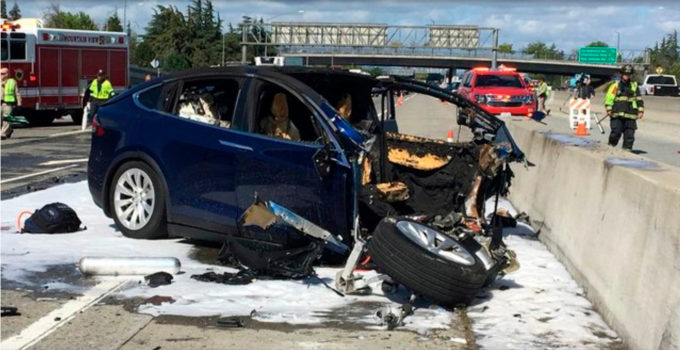
\includegraphics[width=0.45\textwidth, height=4cm]{crash_t}
  }
  \subfigure[车祸2]{
          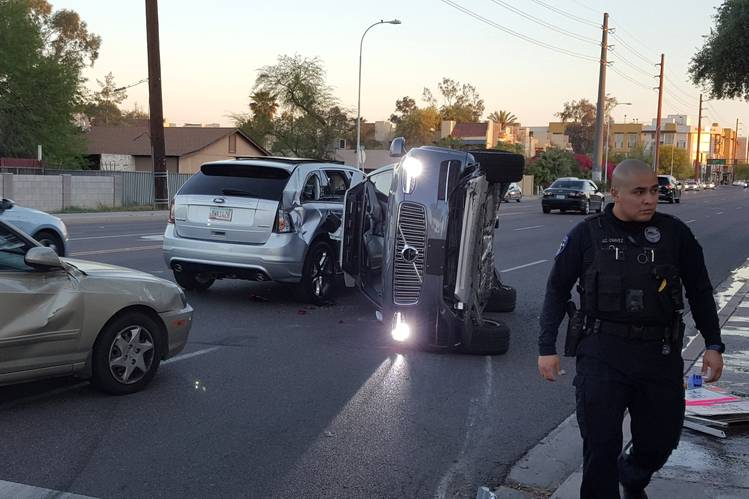
\includegraphics[width=0.45\textwidth, height=4cm]{crash_u}
  }
  \caption{crashs}
\end{figure}

除了上述之外,近年来还陆续有自动驾驶相关的车祸发生,以上种种都表明当前的自动驾驶的安全性能并没有人们认为的那么高。为了提升自动驾驶系统的安全等级,工业界和学术界都在此做了很多研究,于2017年学术界在此领域先后发表了2篇重要的文章,DeepXplore\cite{DeepXplore}和DeepTest\cite{DeepTest},DeepXplore提出了一套深度学习系统测试用例自动生成的框架。DeepTest延伸了DeepXplore的工作并将前者的方法成功的运用到了自动驾驶系统测试用例,即驾驶路况场景图,生成中,两者的工作都以现实的自动驾驶框架为测试对象,成功生成除了很多自动驾驶系统会误判的测试用例,这对提升自动驾驶系统的安全性能有着重大意义。

基于DeepXplore和DeepTest的工作,我所在的实验室提出了DeepRoad\cite{DeepRoad},它借助对抗生成网络\cite{GAN}中的UNIT\cite{UNIT}框架提升了生成的自动驾驶测试用例,即驾驶场景图片的质量。在本论文中,我们做了针对现有的深度学习技术,主要包含对抗生成网络和图像风格转换技术,做了大量的实证研究,以探讨哪个已有的深度学习技术对于自动驾驶测试用例生成,即驾驶场景图片的合成,是最有效的。

本工作希望能为之后的自动驾驶系统测试人员在选择驾驶场景图片测试用例自动生成的框架选择上可以给出一些有价值的建议。

\end{cabstract}

\begin{eabstract}
  In recent years, thanks to the development of deep learning, the research and development of autonomous driving has also made great breakthroughs. Many companies at home and abroad have developed their own autopilot system frameworks, such as Google's Waymo, Baidu's Apollo and Tesla's Autopilot. The most well-known Autopilot has been successfully deployed in real-life commercial Tesla sedan. in.

  Although major companies have advertised that the safety of today's autopilot systems is high enough, several autopilot accidents in the past year or two have caused concern about the safety performance of autopilot systems. The picture on the left is in March 2018. On the 23rd, a car accident occurred on the Highway in Mountain View, California, USA. The post-accident analysis pointed out that the car accident caused the failure of Autopilot to identify the white fence on the gray road background. The same right picture is also due to a misjudgment of the autopilot system developed by Uber, which occurred in 2017 in a car accident in Temple City, Arizona, USA.

  In addition to the above, there have been autopilot-related car accidents in recent years, all of which indicate that the current safety of autonomous driving is not as high as people think. In order to improve the safety level of the automatic driving system, the industry and academia have done a lot of research here. In 2017, the academic community has published two important articles in this field, DeepXplore\cite{DeepXplore} and DeepTest\cite{ DeepTest}, DeepXplore proposes a framework for automatic generation of test cases for deep learning systems. DeepTest extends DeepXplore's work and successfully applies the former method to the autopilot system test case, that is, the driving road scene graph, the generation, both work are based on the actual auto-driving framework as the test object, successfully generated in addition to many automatic Test cases that are misjudged by the driving system are of great significance for improving the safety performance of the autonomous driving system.

  Based on the work of DeepXplore and DeepTest, my lab has proposed DeepRoad\cite{DeepRoad}, which enhances the generated autopilot test case by using the UNIT\cite{UNIT} framework in the anti-generation network \cite{GAN}. The quality of the driving scene picture. In this paper, we have done a lot of empirical research on existing deep learning techniques, including anti-generation network and image style conversion techniques, to explore which existing deep learning techniques are used for autopilot test case generation. That is, the synthesis of the driving scene picture is the most effective.

  This work hopes to give some valuable suggestions for the subsequent autopilot system testers to choose the framework of the auto-generated framework for driving scene picture test cases.
\end{eabstract}

% word count ~ 1000
 % 封面
\makecover
% \input{front/denotation}%物理量名称表,符合规范为主,有要求添加
%\cleardoublepage  自定义在什么位置进行右翻页
\tableofcontents    % 中文目录
%\cleardoublepage  自定义在什么位置进行右翻页
% \tableofengcontents % 英文目录,硕本不要求

\mainmatter
%\linenumbers %debug 选项
%\layout %debug 选项
%\floatdiagram %debug 选项
%\begin{figure} %debug 选项
%\currentfloat %debug 选项
%\tryintextsep{\intextsep} %debug 选项
%\trytopfigrule{0.5pt} %debug 选项
%\trybotfigrule{1pt} %debug 选项
%\setlayoutscale{0.9} %debug 选项
%\floatdesign %debug 选项
%\caption{Float layout with rules}\label{fig:fludf} %debug 选项
%\end{figure} %debug 选项
% % !Mode:: "TeX:UTF-8"
\newcommand{\specialcell}[2][c]{%
  \begin{tabular}[#1]{@{}c@{}}#2\end{tabular}}
\newcommand{\mthead}[1]{\textit{\textbf{#1}}}

\newcommand{\newmodel}[1]{\textbf{#1.}\cite{#1}\quad}

\chapter{绪论}[Introduction]

\section{背景}[Background]

虽然目前很多公司都开发了自己的自动驾驶系统,但其使用的技术几乎都是基于计算机视觉,目标检测,目标识别等深度学习、机器学习技术。因此,针对自动驾驶系统的测试技术也是源于深度学习系统的测试技术。其中,在基于深度神经网络的自动驾驶系统中,其神经网络模型将被汽车的各种传感器(雷达、摄像头等)接收到的数据作为输入,经过其控制系统,通常为深度神经网络,的运算处理后输出各种驾驶行为(方向盘拐角、刹车信号,速度控制信号等)。下图\ref{as_example}展示了一个基于卷积神经网络的自动驾驶系统例子,这个系统由输入(摄像头拍摄的图像)、输出层(方向盘拐角)和中间的隐藏层组成。本章主要讲述传统的深度学习测试技术以及目前学术界比较推崇的自动测试技术。

\begin{figure}[h]
    \centering
    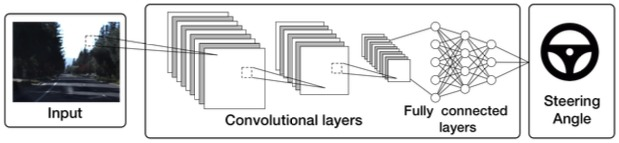
\includegraphics[width=0.8\textwidth]{as_example}
    \caption{基于卷积神经网络的自动驾驶系统\cite{DeepRoad}}
    \label{as_example}
\end{figure}

\subsection{传统的深度学习系统测试技术}[The traditional testing technology of DNN]

深度神经网络,通常指一个元组$N=(L,T,\Theta)$,这里$L=\{L_k|k\in \{1..K\}\}$代表一组网络层,$T\subseteq L\times L$代表各层之间的连接组合,$\Theta=\{\theta_k|k\in \{2,...,K\}\}$代表一组函数,每个函数代表非输入层的激活函数。在一个深度神经网络中,$L_1$指输入层,$L_K$指输出层,其他的层叫做隐藏层。每一层$L_k$由$s_k$个神经元组成,$k$层的第$l$个神经元记为$n_{k,l}$,每个神经元$n_{k,l},1\lt k \lt K, 1\leq l\leq s_k$跟两个变量相关$u_{k,l}$和$v_{k,l}$,分别表示神经元在经过激活函数处理前后的值。目前ReLU\cite{relu}函数是用在深度神经网络中当前最流行的激活函数,根据该函数隐藏层中的每个神经元的激活值可以定义为
\begin{gather}
    v_{k,l}=ReLU(u_{k,l})=\begin{cases}
        u_{k,l} & if\quad u_{k,l} \geq 0 \\
        0 & otherwise
    \end{cases}
\end{gather}
每个输入节点$n_{1,l}\leql 1 \leq s_1$都跟一个变量$v_{1,l}$有关,每个输出节点$n_{K,l},1\leq \leq s_K$跟变量$u_{K,l}$相关,因为已经没有激活函数可以作用在它们身上了。 

除了输入节点,其它的神经元都通过特定的参数跟下一层中的神经元相连接,令所有$k$和$l$都满足$2\leq k \leq K, 1\leq l \leq s_k$,则有
\begin{gather}
u_{k,l}=b_{k,l}+\sum_{1\leq h\leq s_{k-1}}w_{k-1,h,l}\dot v_{k-1,h}
\end{gather} 
这里$w_{k-1,h,l}$为$n_{k-1,h}$和$n_{k,l}$之间连接的权值,$b_{k,l}$称作神经元$n_{k,l}$的偏执项。这个定义可以表示全连接函数和卷积函数。函数$\theta_k$是上面两个公式的组合。得益于ReLU函数的使用,神经网络表现的行为是高度非线性的。

最后,对于任意输入,深度神经网络都有一个对应的标记,即对于该输入,输出层中拥有最大值的神经元下标:$label=\max_{1\leq l\leq s_K}u_{K,l}$。令$L$为标记的集合。

下图\ref{fig:dnn}为一个4层神经网络的例子,它的输入空间是$D_{L_1}=\mathbb{R}^2$,这里$\mathbb{R}$指整个实数集。
\begin{figure}[h]
    \centering
    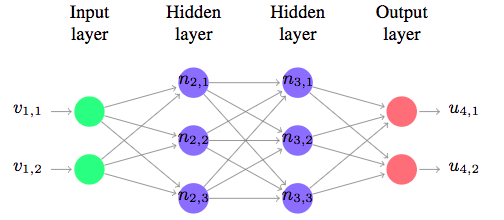
\includegraphics[width=.6\textwidth]{dnn_4}
    \caption{一个4层神经网络}
    \label{fig:dnn}
\end{figure}

深度学习技术是一种通过研究同类大量数据的表征,对未知新数据的特征进行推测的一门技术。在其行使职能,即预测新数据特征前,必须要学习大量同类的数据,即模型训练。模型训练完成后为了提前检测模型的准确性,会在之前的训练数据集中保留一部分数据,作为训练结束后的模型的测试数据集,使其在未被学习过的测试数据集上进行预测,最后以测试数据集上的准确性作为训练好的模型的精准度。目前学术界公认理想的训练数据集与测试数据集占比分别为70\%和30\%\cite{cs231n}。

其训练过程通常是以神经元为基本单位的神经网络为基本架构,采用向后传播算法来自动学习调节网络中的权值参数,训练过程中对权值初始数值的设置以及其他的初始训练参数的设置也十分重要,如果设置不当会有梯度消失,收敛时间过长等问题,当然训练数据集对训练结果的影响也很大。数据集的具体数量跟模型处理的具体问题相关,一般来说,处理的问题越复杂,即数据的特征越多,需要的数据量也就越多,比如比较出名的ImageNet\cite{ImageNet}比赛,公开可用的数据集多达1500万张由人工标注的图片数据。对于自动驾驶,也有诸多开源数据集,比如Oxford RobotCar\cite{ds:oxford},Comma.ai\cite{ds:ai},Udacity\cite{udacity_dataset},Berkeley大规模自动驾驶视频数据集\cite{ds:berkeley},Cityscape\cite{Cordts2016Cityscapes}等。深度学习技术对已有数据特征拟合的本质和其训练测试的过程导致其对数据量的严重依赖,传统的深度学习测试需要大量的人工收集、标注数据,着极度的增加了其中的人力成本。除此之外,传统的通过人工收集数据的方式有严重的缺点,即收集到的数据无法保证覆盖到了所有可能的极端场景,以自动驾驶测试数据集为例,人工收集的数据集一般是车载记录仪记录的道路驾驶视频图片,但一般大雨、大雪等极端天气场景数据很少也很难收集,这就给相应的极端场景自动驾驶系统测试带来了不确定性。 

\subsection{针对深度学习和自动驾驶的软件测试研究}

针对上诉问题,学术界提出了DeepXplore,在此其基础上,针对自动驾驶的软件测试,进一步提出了DeepTest和DeepRoad实现了深度学习系统测试用例自动生成系统来缓解深度学习系统对于数据量的依赖。除此外,针对训练数据集数量可能不够等问题,还有DeepMutation\cite{DeepMutation}、DeepCover\cite{DeepCover}等工作被提出。下面对以上几项针对深度学习和自动驾驶系统的软件测试技术和传统的软件测试做一个简单的介绍。

\subsubsection{传统的软件测试技术}

传统的软件测试方法可粗略地分为黑盒测试和白盒测试两大类。黑盒测试主要针对测试软件的功能是否如预期运作,而不关心软件内部逻辑结构的运行是否合理等。测试者将软件当做一个黑箱,只指定输入,然后观察软件的输出是否正确。白盒测试则与黑盒测试相反,它主要关心的是程序软件内部逻辑是否运行如预期,重点测试软件内部的部件功能,是基于系统内部部件行为分析的测试方法,常常被用在单元测试和集成测试中。除此外,在传统的软件测试技术中还有一个重要的指标:测试/代码覆盖率,该指标常被用来描述当程序运行一个特定的测试用例时,程序里被执行到的代码部分,通常以百分比的形式表示,测试用例有较高的代码覆盖率的程序存在BUG的概率会小于代码覆盖率低的程序。下面讲到的现主流深度学习测试技术多数属于白盒测试的范畴。

\subsubsection{DeepXplore}[DeepXplore]
DeepXplore首先指出了深度学习系统与传统的软件开发系统的不同:传统软件的开发人员直接指定软件系统的逻辑,然而深度学习则是从数据特征中“学习、推到”它们的运行规则,甚至对于深度学习系统的开发人员来说,他们都不一定清楚训练好的深度学习模型的确切运行逻辑。因此DeepXplore
不是直接寻找深度学习系统中的逻辑错误,而是通过自动产生、寻找一些能使多个同类深度学习系统做出不同行为判断的测试用例,并通过这些触发被测试的DNN系统针对同一测试用例产生不同行为判断的行为推测出被测试系统中必有一个或多个系统存在BUG行为,然后并将这些找到的测试用例放回原训练数据集里重新训练模型,试图修正之前错误的行为。

除了将使不同的DNN系统做出不同预测行为为目标外,DeepXplore也借鉴了传统软件测试技术中的代码覆盖率的概念,为了使得尽可能测试整个DNN系统,DeepXplore引入了神经元覆盖率的概念,即测试用例测试过程中,在整个深度学习系统中,被“激活”,即输出值超过了某个阀值的神经元的个数占整个网络结构神经元总数的占比。与代码覆盖率类似,我们期望神经元覆盖率越高越好。

DeepXplore以神经元覆盖率和使得不同DNN系统输出不一致为目标,将在原始测试用例上的修改抽象成为一个优化算法,使用梯度上升算法,最后自动生成一些使得被测的DNN系统得到不同的预测值,且各个DNN系统的神经元覆盖率很高的测试用例,DeepTest基于DeepXplore的工作,提出了一套专门针对自动驾驶系统,能够自动检测出错误行为的测试系统。发生在自动驾驶系统上的车祸大部分都是发生在一些罕见的路况场景下,而传统的自动驾驶检测测试技术几乎是完全依赖大量的罕见路况场景图片的人工收集与标注,这不仅包含了大量的人工成本,重要的是人工收集的数据无法保证能够覆盖度到了所有的极端场景数据。这些极端场景就好像是传统软件中的BUG,但是这些BUG一旦被检测到,就可能通过把这些导致错误的输入重新放入训练集,同时改变一下模型的结构和参数来修复。DeepTest正是通过以上的思路来设计的一套自动测试系统。

\begin{algorithm}[h]
    \small
    \SetAlgoLined
    \SetKwInOut{Input}{Input}
    \SetKwInOut{Output}{Output}
    \SetKwInOut{Variable}{Variable}

    \Input{Transformations T, Seed Images I}
    \Output{Generated Test Cases}
    \Variable{S: Stack to save outputs; Tqueue: Queue to save transformations}

    push all seed imgs to Stack S;\;
    $genTests = \varnothing$\;
    \While{S is not empty}{
        img = S.pop()\;
        $Tqueue = \varnothing$\;
        numFailedTries = 0 \;
        \While{$numFailedTries \leq maxFailedTries$}{
            \eIf{$Tqueue\ is\ not\ empty$}{
                T1 = Tqueue.deque()
            }{
                Randomly pick transformations T1 from T
            }
            Randomly pick parameter P1 for T1\;
            Randomly pick transformation T2 from T\;
            Randomly pick parameter P2 from T2\;
            newImage = ApplyTransforms(image, T1, P1m T2, P2)\;
            \eIf{covInc(newiamge)}{
                Tqueue.enqueue(T1)
                Tqueue.enqueue(T2)
                UpdateCoverage()
                $genTests=genTests \cup newiamge S.push(newImage)$
            }{
                $numFailedTries=numFailed++$
            }
        }
    }
    return genTests
    \caption{混合变换优化算法\cite{DeepTest}}
    \label{alg1}
\end{algorithm}

具体的实现上,DeepTest依旧借用DeepXplore提出的神经元覆盖率的概念,使用位移、拉伸、仿射以及直接修改像素的透明度等基本的图形变换的手段来合成新的驾驶图像,文章里提到合成后的数据能使原DNN系统的神经元覆盖率提升100\%\cite{DeepTest},并以提升神经元覆盖率为目标,给出了一个优化算法\ref{alg1},以获得最佳的图像混合变换,最后DeepTest在利用这些合成的新数据重新训练自动驾驶模型来提高模型对于极端场景的鲁棒性。

\subsubsection{DeepRoad}[DeepRoad]

尽管DeepTest已经提出了一个较为完善的自动驾驶系统测试方案,以相对便宜和简洁的方法,利用大量的原始和合成出来的驾驶场景图片成功地检测出了许多自动驾驶系统前后不一致的驾驶行为,但它有一个很严重的缺陷:DeepTest用来合成图片的技术很难合成一些能够精确反映现实驾驶场景的图片,并且现实驾驶场景的图片也很难由一些基础的仿射、位移变换模拟合成出来,其用来模拟雨天、雾天的场景的技术仅仅是在原始图层上添加一层额外的图层,如下图\ref{label-deeptest}所示,对于雾天,DeepTest仅仅是加了一层白色的图层,对于雨天,加了一层线条层。很明显这些合成图离现实中真实的驾驶场景有较大的差别。从另一个角度来说,即使用这些图检测出了自动驾驶系统错误的驾驶行为也很难有说服力,因为这些“出错”的场景在现实中根本不会出现。其实很多可能的真实的驾驶场景根本不能用一些简单的图像处理技术来模拟合成。

\begin{figure}[h]
    \centering
    \subfigure[DeepTest]{
        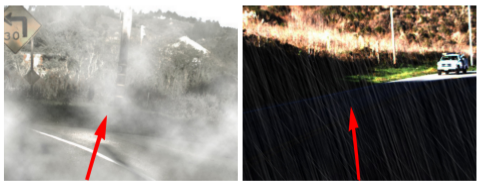
\includegraphics[width = 0.7\textwidth]{deeptest_effect}
    }
    \subfigure[DeepRoad]{
        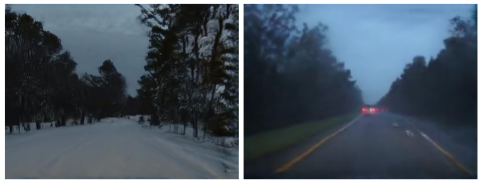
\includegraphics[width = 0.7\textwidth]{deeproad_effect}
    }
    \caption{天气场景合成效果图比较}
    \label{label-deeptest}
\end{figure}

为了能够自动地合成大量真实的驾驶场景图片,DeepRoad提出了一个半监督合成的框架,抛弃了DeepTest用到的简单的图像处理技术来合成图像,采用深度学习对抗生成网络的技术来合成相对较真实的驾驶场景图片,下图\ref{label-deeptest}为DeepTest合成图和DeepRoad使用对抗生成网络中UNIT\cite{UNIT}框架合成图的效果对比,其中图a红色箭头为自动驾驶系统对该驾驶场景输出的方向盘拐角。可以清楚的看到使用UNIT技术合成的效果比较好的驾驶场景图已经与真实场景很接近了。下图\ref{deeproad_wf}展示了DeepRoad框架的整体流程。

\begin{figure}[h]
    \centering
    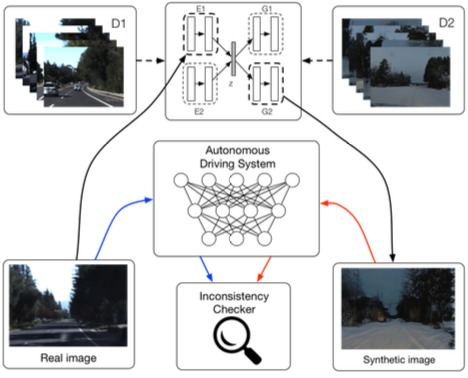
\includegraphics[width=0.75\textwidth]{deeproad_wf}
    \caption{DeepRoad框架流程图\cite{DeepRoad}}
    \label{deeproad_wf}
\end{figure}

DeepRoad将两种天气情况下的图片作为训练输入数据集,训练无监督对抗生成网络UNIT\cite{UNIT}框架,然后利用训练好的UNIT框架对未知新的输入数据进行转换合成,最后测试自动驾驶系统对使用UNIT进行转换后的图片做出的驾驶行为与未转换之前的原始图片的驾驶行为是否一致。

\subsubsection{DeepMutation}

深度学习系统的训练过程决定了其内部的系统逻辑很大程度上由其训练数据集决定,评价深度学习系统模型的标准方法是检测其在测试数据集上的性能水平。因此测试数据集的质量对于我们对模型的信任度至关重要。在数量不够的测试集即使上取得了高准确率,也缺少一般性和鲁棒性。在传统软件测试中,变异测试(Mutation Testing)对于评估测试集质量是一个相当成熟的技术,但是由于深度学习系统和传统软件的本质上的差异使得变异测试无法直接应用于深度学习软件系统中。DeepMutation提出了一个专门针对深度学习系统,评估其测试数据集质量的框架。它借用变异测试中本质思想,首先定义了一套源码级的变异操作子,对深度学习系统软件源码注入错误。进一步地,设计了一套模型级的变异操作子,比如对模型的神经网络层数进行增删操作,以及对单层网络的神经元进行增删操作,无须训练过程直接对深度学习系统注入错误。最终,测试数据集的质量可以根据注入的错误能被多大程度的检测出来分析得出。

\subsubsection{DeepCover}

传统的软件测试通过设置诸如代码覆盖率等指标来指示测试数据集的自动生成方向,但由于深度神经网络系统缺少类似传统软件的结构和逻辑控制流,因此如何为它们定义譬如分支覆盖率的指标并没有一个十分明显的方向。DeepCover\cite{DeepCover}对于深度神经网络系统提出了一个白盒测试方法,其中包含了一套测试覆盖指标和测试用例生成算法,即利用线性规划,通过扰动给定的测试用例来合成新的测试用例,弥补了传统软件和深度神经网络系统在这一方面的差异。

\subsubsection{NeVer}

NeVer\cite{dsv}提出了一个方法来验证神经网络系统安全性能。它主要关注的是多层神经元网络结构,定义了给定对于任意给定的输入值,其网络输出都保证在已知的范围内,则视该网络为“安全的”。进而NeVer还提出了一套启发式修复算法,能够自动提高测试的神经网络系统安全性能。

\subsection{其他的图像转换技术}[Other Image Transformation Technologies]

DeepRoad提出的将深度学习技术运用到自动驾驶系统测试用例合成,并设计的一套自动测试的框架在检测自动驾驶系统的稳定性和鲁棒性上,在其实验检测出了大量的现实自动驾驶系统有误的驾驶行为的结果\cite{DeepRoad}上看是有效的。其相对前人的工作DeepTest主要的改进是将测试用例的合成技术,即驾驶场景的图像转换技术,由原有的基本的图像变换换成了深度学习中的对抗生成网络技术。我们在利用UNIT合成驾驶场景图的实验过程中发现,虽然有效果比较好的合成图,但其占总的合成图的比例很小,1万张结果图中比较真实的图像大约有30多张,大部分的结果图如下,可以看到效果比较差,我们分析了效果比较差的原因主要是使用的训练数据集是由我们从Youtube上爬取的视频制作的数据图像,与UNIT官方使用的NVIDIA公司提供的闭源数据集相差比较大导致。

但其实目前学术界和工业界已经提出的能够进行不同天气场景图像转换的深度学习技术有很多。对此我们进行了调研,发现主要有两大类:对抗生成网络和图像风格转换(Neural Style Transfer)。以上两类技术的实现都是利用了神经网络的架构,这也是目前这类技术的主流模式。但除此之外还有很多没有使用诸如卷积神经网络架构的图像风格转换技术。这里有代表性的技术由基于笔画、线条进行渲染的技术。通常指通过一个对只有线条的画进行处理,最终渲染合成出一张具有某种风格的图像。这类算法的主要目的是根据有限的信息合成一张具有特定风格的图像。基于样例的渲染技术也属于没有采用神经网络架构实现图像合成的技术,这类算法通常会根据已有数据学习源数据到目标风格图片之间的映射函数,然后根据学习到的函数通过监督学习的方式将输入图片转换到目标风格图像空间上,从而实现图像的风格转换。

我们对DeepRoad进行的实验也表明在得不到理想的训练数据集的情况下利用UNIT进行图像转换的实验结果是不理想的,那么可否将UNIT更换为其他的能够进行图像转换的深度学习技术?哪一种技术的实现效果是最好的?如何评价各种图像转换技术在合成驾驶场景图上的好坏?哪一种技术的训练成本和实现成本是最小的?针对以上问题,我们对现有的能够实现图像风格转换的深度学习技术展开实证研究,希望能够找到答案,最终可以为以后的自动驾驶系统测试人员在选择驾驶场景图片测试用例的合成技术框架上提供一些有帮助的建议。

% TODO UNIT图像

\section{自动驾驶技术的发展}

本小节简要介绍自动驾驶技术的发展历程。

涉及自动驾驶技术的最早实验起始于1925年\cite{auto-driving-history}。在美国纽约,一辆名为“American Wonder”的无线电控制汽车从百老汇大姐驶过第五大道,它通过无线电接收器接受来自另一辆载人,并发出无线电信号的车辆引导行驶。自动引导驾驶行为的驾驶技术最早出现于1939年的万国博览会上,展出了一辆同样无线电控制汽车,由内嵌在公路里的芯片提供的电磁信场进而驱动车辆行驶。1958年,General Motors在此基础上提出了改进方案,在汽车的前部添加了能够检测到流过内嵌在公路内线路电流的电线圈,该电流可以被人为控制,进而影响汽车的方向盘转向。1977年,日本在此方案上作了进一步的改进,他们使用了一套能够将路况图像数据传输到计算机处理的摄影系统,但是装备了这套系统的车辆在当时最高时速只有20公里。10年后德国人同样使用了名为VaMoRs的摄影影像系统,并将汽车的最高时速提升到了56公里。 

\begin{figure}[ht]
    \centering
    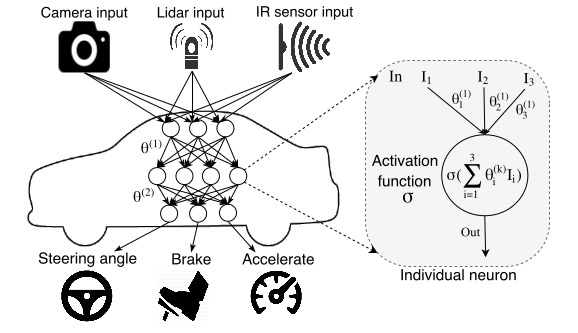
\includegraphics[width=0.8\textwidth]{auto-driving-sys}
    \caption{基于深度学习的自动驾驶系统}
    \label{auto-driving-sys}
\end{figure}

近年来,得益于深度学习技术的发展,基于深度学习的自动驾驶系统在对环境的感知和应对能力上也取得了许多突破,如上图\ref{auto-driving-sys}所示,目前的自动驾驶系统大致课分为3个部分,分别是负责接受外界数据的传感器单元,一般由摄像头、雷达和红外探测器组成。第二部分是系统的控制单元,它一般由多个神经元构成的多层神经网络组成,主要负责处理传感器接受的数据,利用诸如计算机视觉,物体检测,物体追踪等深度学习技术,最终输出一系列汽车控制信号,比如方向盘拐角信号、汽车油门信号和刹车信号等,达到汽车控制的目的。最后是汽车的实体功能单元。在本论文中,针对自动驾驶系统控制单元的研究,我们主要关注的输入是摄像头拍摄的路况图片,输出主要关注方向盘拐角信号。目前国内外许多公司开发的自动驾驶系统,比如Google公司的Waymo,Baidu公司的Apollo以及Tesla公司的Autopilot都是基于此类架构。

\section{自动驾驶系统测试技术国内外研究现状}

Pei K\cite{DeepXplore}等人首次针对自动驾驶系统测试,提出一个自动测试系统DeepXplore,基于已有的测试数据集自动生成新的,能够使测试的深度学习系统“出错”的测试用例,在深度学习系统测试用例自动生成框架领域具有里程碑的意义。时隔一年,Pei K同组的人基于DeepXplore的工作继续提出了DeepTest\cite{DeepTest}框架,其去掉了DeepXplore框架必须提供多个类似功能的深度学习系统的要求,同时针对自动驾驶系统测试用例的自动生成做了许多改动。至此,相对之前的深度学习测试技术来说,一个代价低廉,有效的测试系统框架基本行程。虽然文献\cite{DeepTest}将自动驾驶系统测试列为了DeepTest的使用场景之一,但是直接将DeepTest使用在自动驾驶系统测试用例合成上仍有许多致命的缺陷,最为明显的就是其测试用例合成技术,即驾驶场景图片合成技术使用的是基础的图像转换技术,使用这类技术合成的照片通常情况下离真实场景的图片有不小的差别,再者,许多真实的极端天气场景的路况图片,比如大雨、大雪天气的路况图片是无法使用基础的图片转换技术来模拟合成的。

针对上述DeepTest的问题,我所在的实验室于18年提出了将深度学习技术使用在自动驾驶测试用例合成上,借此提出了DeepRoad框架\cite{DeepRoad}。DeepRoad使用的深度学习技术是属于对抗生成网络大类中的UNIT\cite{UNIT}框架。除了使用UNIT来合成驾驶场景图片外,来自NVDIA公司的Ming-Yu Liu等人与2016年相继提出了MUNIT\cite{MUNIT},Fast Photo Style\cite{fps}等技术利用卷积神经网络等架构同样实现了不同天气场景路况图片的转换。总体来说,图像风格转换技术的研究目前在国内外都处于一个比较活跃的阶段。


\section{本论文研究内容及创新点}

\subsection{本文主要研究内容}

车辆是人类的一项伟大发明,它极大的便利了人类的交通出行,使人类对于长途的旅行摆脱了以原始低效的步行和动物驼行为主的出行方式。但它在给予人类极大便利的同时,每年不断增长,死于汽车交通事故的人数就像一把达摩利斯双刃剑在不断地威胁着人类的出行安全。据世界卫生组织(WHO)发布的全球道路安全状况报告\cite{who}显示,我国每年因交通事故死亡的人数已超过了25万,平均每10万人口死亡的人数为18.8。严峻的事实使得人们致力于研究各种能够提高交通安全的技术。美国交通安全局的网站\cite{usdt}显示:2018年在美国发生的致命车祸中,有94\%的事故是由于人类的各种不规范驾驶行为导致。而近年来发展迅猛的自动驾驶技术正是解决困扰人们已久的交通驾驶安全问题的一个很好的解决方案。

虽然自动驾驶技术已经发展相对成熟,但近年来世界各地发生的几起跟自动驾驶相关的车祸揭示了该技术在安全性能上仍有不可忽视的隐患,本文的内容正是基于以上背景,介绍了目前学术界提出的几种自动驾驶系统测试框架,并基于前人的工作,
\begin{enumerate}
    \item \textbf{提出了DeepRoad,一个面向深度神经网络自动驾驶系统的蜕变测试框架。}
    \item \textbf{针对DeepRoad生成的测试用例只有雪天和雨天场景的路况图像,探索了其他能够实现自动驾驶系统测试用例自动合成的深度学习技术(即能实现各种天气场景路况图像转换的技术),并对每种技术模型的实验数据进行统计和总结。}
    \item \textbf{针对各个模型的实验数据总结了3个可用于评价生成测试用例质量和模型性能的指标:FID值,方向盘拐角偏差和模型训练时长,针对每个指标对各个模型的对应的性能进行了评价并得出了相应的结论。}
\end{enumerate}

\subsection{本文主要创新点及贡献}

\begin{enumerate}
    \item \textbf{将传统软件工程领域的蜕变测试技术引入到了基于深度神经网络的自动驾驶系统测试工作中,提出的DeepRoad测试框架在测试系统鲁棒性,以及寻找能体现系统不稳定性的不一致驾驶行为数目上都由于前人的工作(DeepTest)}
    \item \textbf{首次将深度学习技术应用到了自动驾驶系统测试用例的合成上,提高了生成的测试用例质量,扩充了测试用例覆盖范围,进一步降低了测试用例数据的收集成本}
    \item \textbf{基于DeepRoad的工作,针对测试用例的合成技术进行了进一步的探索研究,将更多的深度学习技术,主要是对抗生成网络和神经风格迁移技术应用到了测试用例的合成上,在对各个模型生成的测试用例观察后,得到了一些经验性的结论。}
\end{enumerate}
 
% !Mode:: "TeX:UTF-8"
\newcommand{\specialcell}[2][c]{%
  \begin{tabular}[#1]{@{}c@{}}#2\end{tabular}}
\newcommand{\mthead}[1]{\textit{\textbf{#1}}}

\newcommand{\newmodel}[1]{\textbf{#1.}\cite{#1}\quad}

\chapter{绪论}[Introduction]

\section{背景}[Background]

虽然目前很多公司都开发了自己的自动驾驶系统,但其使用的技术几乎都是基于计算机视觉,目标检测,目标识别等深度学习、机器学习技术。因此,针对自动驾驶系统的测试技术也是源于深度学习系统的测试技术。其中,在基于深度神经网络的自动驾驶系统中,其神经网络模型将被汽车的各种传感器(雷达、摄像头等)接收到的数据作为输入,经过其控制系统,通常为深度神经网络,的运算处理后输出各种驾驶行为(方向盘拐角、刹车信号,速度控制信号等)。下图\ref{as_example}展示了一个基于卷积神经网络的自动驾驶系统例子,这个系统由输入(摄像头拍摄的图像)、输出层(方向盘拐角)和中间的隐藏层组成。本小节主要讲述自动驾驶技术几研究、相关的测试技术以及本工作所用要的研究方法:软件工程领域的实证研究。

\begin{figure}[h]
    \centering
    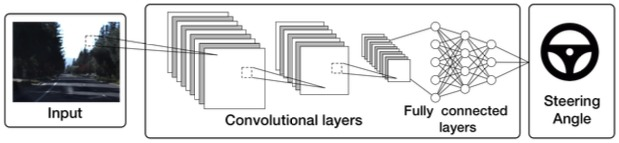
\includegraphics[width=0.8\textwidth]{as_example}
    \caption{基于卷积神经网络的自动驾驶系统\cite{DeepRoad}}
    \label{as_example}
\end{figure}

\subsection{自动驾驶技术及研究}

涉及自动驾驶技术的最早实验起始于1925年\cite{auto-driving-history}。在美国纽约,一辆名为“American Wonder”的无线电控制汽车从百老汇大姐驶过第五大道,它通过无线电接收器接受来自另一辆载人,并发出无线电信号的车辆引导行驶。自动引导驾驶行为的驾驶技术最早出现于1939年的万国博览会上,展出了一辆同样无线电控制汽车,由内嵌在公路里的芯片提供的电磁信场进而驱动车辆行驶。1958年,General Motors在此基础上提出了改进方案,在汽车的前部添加了能够检测到流过内嵌在公路内线路电流的电线圈,该电流可以被人为控制,进而影响汽车的方向盘转向。1977年,日本在此方案上作了进一步的改进,他们使用了一套能够将路况图像数据传输到计算机处理的摄影系统,但是装备了这套系统的车辆在当时最高时速只有20公里。10年后德国人同样使用了名为VaMoRs的摄影影像系统,并将汽车的最高时速提升到了56公里。 

\begin{figure}[ht]
    \centering
    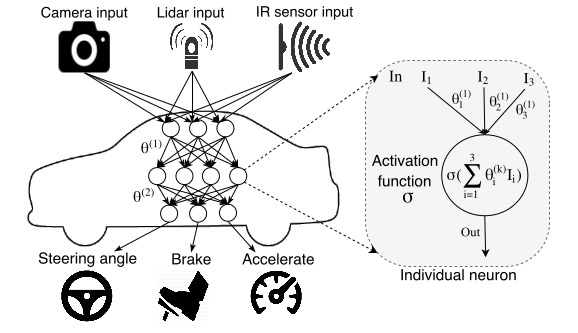
\includegraphics[width=0.8\textwidth]{auto-driving-sys}
    \caption{基于深度学习的自动驾驶系统}
    \label{auto-driving-sys}
\end{figure}

近年来,得益于深度学习技术的发展,基于深度学习的自动驾驶系统在对环境的感知和应对能力上也取得了许多突破,如上图\ref{auto-driving-sys}所示,目前的自动驾驶系统大致课分为3个部分,分别是负责接受外界数据的传感器单元,一般由摄像头、雷达和红外探测器组成。第二部分是系统的控制单元,它一般由多个神经元构成的多层神经网络组成,主要负责处理传感器接受的数据,利用诸如计算机视觉,物体检测,物体追踪等深度学习技术,最终输出一系列汽车控制信号,比如方向盘拐角信号、汽车油门信号和刹车信号等,达到汽车控制的目的。最后是汽车的实体功能单元。在本论文中,针对自动驾驶系统控制单元的研究,我们主要关注的输入是摄像头拍摄的路况图片,输出主要关注方向盘拐角信号。目前国内外许多公司开发的自动驾驶系统,比如Google公司的Waymo,Baidu公司的Apollo以及Tesla公司的Autopilot都是基于此类架构。

\subsection{自动驾驶测试研究}

Pei K\cite{DeepXplore}等人首次针对自动驾驶系统测试,于2017年提出一个自动测试系统DeepXplore,基于已有的测试数据集自动生成新的,能够使测试的深度学习系统“出错”的测试用例,在深度学习系统测试用例自动生成框架领域具有里程碑的意义。时隔一年,Pei K同组的人基于DeepXplore的工作继续提出了DeepTest\cite{DeepTest}框架,去掉了DeepXplore框架必须提供多个类似功能的深度学习系统的要求,同时针对自动驾驶系统测试用例的自动生成做了许多改动。至此,相对之前的深度学习测试技术来说,一个代价低廉,有效的测试系统框架基本行程。虽然文献\cite{DeepTest}将自动驾驶系统测试列为了DeepTest的使用场景之一,但是直接将DeepTest使用在自动驾驶系统测试用例合成上仍有许多致命的缺陷,最为明显的就是其测试用例合成技术,即驾驶场景图片合成技术使用的是基础的图像转换技术,使用这类技术合成的照片通常情况下离真实场景的图片有不小的差别,再者,许多真实的极端天气场景的路况图片,比如大雨、大雪天气的路况图片是无法使用基础的图片转换技术来模拟合成的。

针对上述DeepTest的问题,我所在的实验室于18年提出了将深度学习技术使用在自动驾驶测试用例合成上,借此提出了DeepRoad框架\cite{DeepRoad}。DeepRoad使用的深度学习技术是属于对抗生成网络大类中的UNIT\cite{UNIT}框架。除了使用UNIT来合成驾驶场景图片外,来自NVDIA公司的Ming-Yu Liu等人与2016年相继提出了MUNIT\cite{MUNIT},Fast Photo Style\cite{fps}等技术利用卷积神经网络等架构同样实现了不同天气场景路况图片的转换。由于目前的自动驾驶系统都是基于深度学习技术,因此为了对目前自动驾驶测试技术有更好的了解,下面先介绍一下传统的软件测试技术和深度学习测试技术。

\subsubsection{传统的软件测试技术}

传统的软件测试方法可粗略地分为黑盒测试和白盒测试两大类。黑盒测试主要针对测试软件的功能是否如预期运作,而不关心软件内部逻辑结构的运行是否合理等。测试者将软件当做一个黑箱,只指定输入,然后观察软件的输出是否正确。白盒测试则与黑盒测试相反,它主要关心的是程序软件内部逻辑是否运行如预期,重点测试软件内部的部件功能,是基于系统内部部件行为分析的测试方法,常常被用在单元测试和集成测试中。除此外,在传统的软件测试技术中还有一个重要的指标:测试/代码覆盖率,该指标常被用来描述当程序运行一个特定的测试用例时,程序里被执行到的代码部分,通常以百分比的形式表示,测试用例有较高的代码覆盖率的程序存在BUG的概率会小于代码覆盖率低的程序。下面讲到的现主流深度学习测试技术多数属于白盒测试的范畴。

\subsubsection{传统的深度学习系统测试技术}

深度神经网络,通常指一个元组$N=(L,T,\Theta)$,这里$L=\{L_k|k\in \{1..K\}\}$代表一组网络层,$T\subseteq L\times L$代表各层之间的连接组合,$\Theta=\{\theta_k|k\in \{2,...,K\}\}$代表一组函数,每个函数代表非输入层的激活函数。在一个深度神经网络中,$L_1$指输入层,$L_K$指输出层,其他的层叫做隐藏层。每一层$L_k$由$s_k$个神经元组成,$k$层的第$l$个神经元记为$n_{k,l}$,每个神经元$n_{k,l},1\lt k \lt K, 1\leq l\leq s_k$跟两个变量相关$u_{k,l}$和$v_{k,l}$,分别表示神经元在经过激活函数处理前后的值。目前ReLU\cite{relu}函数是用在深度神经网络中当前最流行的激活函数,根据该函数隐藏层中的每个神经元的激活值可以定义为
\begin{gather}
    v_{k,l}=ReLU(u_{k,l})=\begin{cases}
        u_{k,l} & if\quad u_{k,l} \geq 0 \\
        0 & otherwise
    \end{cases}
\end{gather}
每个输入节点$n_{1,l}\leql 1 \leq s_1$都跟一个变量$v_{1,l}$有关,每个输出节点$n_{K,l},1\leq \leq s_K$跟变量$u_{K,l}$相关,因为已经没有激活函数可以作用在它们身上了。 

除了输入节点,其它的神经元都通过特定的参数跟下一层中的神经元相连接,令所有$k$和$l$都满足$2\leq k \leq K, 1\leq l \leq s_k$,则有
\begin{gather}
u_{k,l}=b_{k,l}+\sum_{1\leq h\leq s_{k-1}}w_{k-1,h,l}\dot v_{k-1,h}
\end{gather} 
这里$w_{k-1,h,l}$为$n_{k-1,h}$和$n_{k,l}$之间连接的权值,$b_{k,l}$称作神经元$n_{k,l}$的偏执项。这个定义可以表示全连接函数和卷积函数。函数$\theta_k$是上面两个公式的组合。得益于ReLU函数的使用,神经网络表现的行为是高度非线性的。

最后,对于任意输入,深度神经网络都有一个对应的标记,即对于该输入,输出层中拥有最大值的神经元下标:$label=\max_{1\leq l\leq s_K}u_{K,l}$。令$L$为标记的集合。

下图\ref{fig:dnn}为一个4层神经网络的例子,它的输入空间是$D_{L_1}=\mathbb{R}^2$,这里$\mathbb{R}$指整个实数集。
\begin{figure}[h]
    \centering
    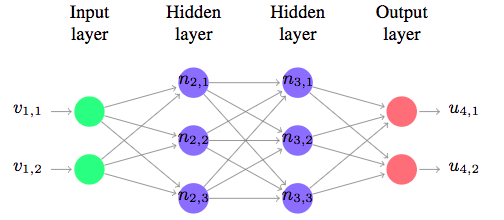
\includegraphics[width=.6\textwidth]{dnn_4}
    \caption{一个4层神经网络}
    \label{fig:dnn}
\end{figure}

深度学习技术是一种通过研究同类大量数据的表征,对未知新数据的特征进行推测的一门技术。在其行使职能,即预测新数据特征前,必须要学习大量同类的数据,即模型训练。模型训练完成后为了提前检测模型的准确性,会在之前的训练数据集中保留一部分数据,作为训练结束后的模型的测试数据集,使其在未被学习过的测试数据集上进行预测,最后以测试数据集上的准确性作为训练好的模型的精准度。目前学术界公认理想的训练数据集与测试数据集占比分别为70\%和30\%\cite{cs231n}。

其训练过程通常是以神经元为基本单位的神经网络为基本架构,采用向后传播算法来自动学习调节网络中的权值参数,训练过程中对权值初始数值的设置以及其他的初始训练参数的设置也十分重要,如果设置不当会有梯度消失,收敛时间过长等问题,当然训练数据集对训练结果的影响也很大。数据集的具体数量跟模型处理的具体问题相关,一般来说,处理的问题越复杂,即数据的特征越多,需要的数据量也就越多,比如比较出名的ImageNet\cite{ImageNet}比赛,公开可用的数据集多达1500万张由人工标注的图片数据。对于自动驾驶,也有诸多开源数据集,比如Oxford RobotCar\cite{ds:oxford},Comma.ai\cite{ds:ai},Udacity\cite{udacity_dataset},Berkeley大规模自动驾驶视频数据集\cite{ds:berkeley},Cityscape\cite{Cordts2016Cityscapes}等。深度学习技术对已有数据特征拟合的本质和其训练测试的过程导致其对数据量的严重依赖,传统的深度学习测试需要大量的人工收集、标注数据,着极度的增加了其中的人力成本。除此之外,传统的通过人工收集数据的方式有严重的缺点,即收集到的数据无法保证覆盖到了所有可能的极端场景,以自动驾驶测试数据集为例,人工收集的数据集一般是车载记录仪记录的道路驾驶视频图片,但一般大雨、大雪等极端天气场景数据很少也很难收集,这就给相应的极端场景自动驾驶系统测试带来了不确定性。 

\subsubsection{自动驾驶测试技术}

针对上诉问题,学术界提出了DeepXplore,在此其基础上,针对自动驾驶的软件测试,进一步提出了DeepTest和DeepRoad实现了深度学习系统测试用例自动生成系统来缓解深度学习系统对于数据量的依赖。除此外,针对训练数据集数量可能不够等问题,还有DeepMutation\cite{DeepMutation}、DeepCover\cite{DeepCover}等工作被提出。下面对以上几项针对深度学习和自动驾驶系统的软件测试技术和传统的软件测试做一个简单的介绍。

\subsubsection{DeepXplore和DeepTest}
DeepXplore首先指出了深度学习系统与传统的软件开发系统的不同:传统软件的开发人员直接指定软件系统的逻辑,然而深度学习则是从数据特征中“学习、推到”它们的运行规则,甚至对于深度学习系统的开发人员来说,他们都不一定清楚训练好的深度学习模型的确切运行逻辑。因此DeepXplore
不是直接寻找深度学习系统中的逻辑错误,而是通过自动产生、寻找一些能使多个同类深度学习系统做出不同行为判断的测试用例,并通过这些触发被测试的DNN系统针对同一测试用例产生不同行为判断的行为推测出被测试系统中必有一个或多个系统存在BUG行为,然后并将这些找到的测试用例放回原训练数据集里重新训练模型,试图修正之前错误的行为。

除了将使不同的DNN系统做出不同预测行为为目标外,DeepXplore也借鉴了传统软件测试技术中的代码覆盖率的概念,为了使得尽可能测试整个DNN系统,DeepXplore引入了神经元覆盖率的概念,即测试用例测试过程中,在整个深度学习系统中,被“激活”,即输出值超过了某个阀值的神经元的个数占整个网络结构神经元总数的占比。与代码覆盖率类似,我们期望神经元覆盖率越高越好。

DeepXplore以神经元覆盖率和使得不同DNN系统输出不一致为目标,将在原始测试用例上的修改抽象成为一个优化算法,使用梯度上升算法,最后自动生成一些使得被测的DNN系统得到不同的预测值,且各个DNN系统的神经元覆盖率很高的测试用例,DeepTest基于DeepXplore的工作,提出了一套专门针对自动驾驶系统,能够自动检测出错误行为的测试系统。发生在自动驾驶系统上的车祸大部分都是发生在一些罕见的路况场景下,而传统的自动驾驶检测测试技术几乎是完全依赖大量的罕见路况场景图片的人工收集与标注,这不仅包含了大量的人工成本,重要的是人工收集的数据无法保证能够覆盖度到了所有的极端场景数据。这些极端场景就好像是传统软件中的BUG,但是这些BUG一旦被检测到,就可能通过把这些导致错误的输入重新放入训练集,同时改变一下模型的结构和参数来修复。DeepTest正是通过以上的思路来设计的一套自动测试系统。

\subsubsection{DeepRoad}

尽管DeepTest已经提出了一个较为完善的自动驾驶系统测试方案,以相对便宜和简洁的方法,利用大量的原始和合成出来的驾驶场景图片成功地检测出了许多自动驾驶系统前后不一致的驾驶行为,但它有一个很严重的缺陷:DeepTest用来合成图片的技术很难合成一些能够精确反映现实驾驶场景的图片,并且现实驾驶场景的图片也很难由一些基础的仿射、位移变换模拟合成出来,其用来模拟雨天、雾天的场景的技术仅仅是在原始图层上添加一层额外的图层,对于雾天,DeepTest仅仅是加了一层白色的图层,对于雨天,加了一层线条层。很明显这些合成图离现实中真实的驾驶场景有较大的差别。从另一个角度来说,即使用这些图检测出了自动驾驶系统错误的驾驶行为也很难有说服力,因为这些“出错”的场景在现实中根本不会出现。其实很多可能的真实的驾驶场景根本不能用一些简单的图像处理技术来模拟合成。

为了能够自动地合成大量真实的驾驶场景图片,DeepRoad提出了一个半监督合成的框架,抛弃了DeepTest用到的简单的图像处理技术来合成图像,采用深度学习对抗生成网络的技术来合成相对较真实的驾驶场景图片,DeepRoad使用了对抗生成网络中UNIT\cite{UNIT}框架来进行路况图像的合成,文献\cite{DeepRoad}实验结果表明合成图较DeepTest的合成图与真实的路况场景更为接近。

DeepRoad的工作原理主要是将两种天气情况下的图片作为训练输入数据集,训练无监督对抗生成网络UNIT\cite{UNIT}框架,然后利用训练好的UNIT框架对未知新的输入数据进行转换合成,最后测试自动驾驶系统对使用UNIT进行转换后的图片做出的驾驶行为与未转换之前的原始图片的驾驶行为是否一致,以此来测试自动驾驶系统的稳定性和鲁棒性。

\subsubsection{DeepMutation}

深度学习系统的训练过程决定了其内部的系统逻辑很大程度上由其训练数据集决定,评价深度学习系统模型的标准方法是检测其在测试数据集上的性能水平。因此测试数据集的质量对于我们对模型的信任度至关重要。在数量不够的测试集即使上取得了高准确率,也缺少一般性和鲁棒性。在传统软件测试中,变异测试(Mutation Testing)对于评估测试集质量是一个相当成熟的技术,但是由于深度学习系统和传统软件的本质上的差异使得变异测试无法直接应用于深度学习软件系统中。DeepMutation提出了一个专门针对深度学习系统,评估其测试数据集质量的框架。它借用变异测试中本质思想,首先定义了一套源码级的变异操作子,对深度学习系统软件源码注入错误。进一步地,设计了一套模型级的变异操作子,比如对模型的神经网络层数进行增删操作,以及对单层网络的神经元进行增删操作,无须训练过程直接对深度学习系统注入错误。最终,测试数据集的质量可以根据注入的错误能被多大程度的检测出来分析得出。

\subsubsection{DeepCover}

传统的软件测试通过设置诸如代码覆盖率等指标来指示测试数据集的自动生成方向,但由于深度神经网络系统缺少类似传统软件的结构和逻辑控制流,因此如何为它们定义譬如分支覆盖率的指标并没有一个十分明显的方向。DeepCover\cite{DeepCover}对于深度神经网络系统提出了一个白盒测试方法,其中包含了一套测试覆盖指标和测试用例生成算法,即利用线性规划,通过扰动给定的测试用例来合成新的测试用例,弥补了传统软件和深度神经网络系统在这一方面的差异。

\subsubsection{NeVer}

NeVer\cite{dsv}提出了一个方法来验证神经网络系统安全性能。它主要关注的是多层神经元网络结构,定义了给定对于任意给定的输入值,其网络输出都保证在已知的范围内,则视该网络为“安全的”。进而NeVer还提出了一套启发式修复算法,能够自动提高测试的神经网络系统安全性能。

\subsection{图像转换技术研究}

DeepRoad提出的将深度学习技术运用到自动驾驶系统测试用例合成,并设计的一套自动测试的框架在检测自动驾驶系统的稳定性和鲁棒性上,在其实验检测出了大量的现实自动驾驶系统有误的驾驶行为的结果\cite{DeepRoad}上看是有效的。其相对前人的工作DeepTest主要的改进是将测试用例的合成技术,即驾驶场景的图像转换技术,由原有的基本的图像变换换成了深度学习中的对抗生成网络技术。我们在利用UNIT合成驾驶场景图的实验过程中发现,虽然有效果比较好的合成图,但其占总的合成图的比例很小,1万张结果图中比较真实的图像大约有30多张,大部分的结果图如下,可以看到效果比较差,我们分析了效果比较差的原因主要是使用的训练数据集是由我们从Youtube上爬取的视频制作的数据图像,与UNIT官方使用的NVIDIA公司提供的闭源数据集相差比较大导致。

但其实目前学术界和工业界已经提出的能够进行不同天气场景图像转换的深度学习技术有很多。对此我们进行了调研,发现主要有两大类:对抗生成网络和图像风格转换(Neural Style Transfer)。以上两类技术的实现都是基于卷积神经网络的架构,这也是目前这类技术的主流模式。但除此之外还有很多没有使用诸如卷积神经网络架构的图像风格转换技术。这里有代表性的技术由基于笔画、线条进行渲染的技术。通常指通过一个对只有线条的画进行处理,最终渲染合成出一张具有某种风格的图像。这类算法的主要目的是根据有限的信息合成一张具有特定风格的图像。基于样例的渲染技术也属于没有采用神经网络架构实现图像合成的技术,这类算法通常会根据已有数据学习源数据到目标风格图片之间的映射函数,然后根据学习到的函数通过监督学习的方式将输入图片转换到目标风格图像空间上,从而实现图像的风格转换。

我们对DeepRoad进行的实验也表明在得不到理想的训练数据集的情况下利用UNIT进行图像转换的实验结果是不理想的,那么可否将UNIT更换为其他的能够进行图像转换的深度学习技术?哪一种技术的实现效果是最好的?如何评价各种图像转换技术在合成驾驶场景图上的好坏?哪一种技术的训练成本和实现成本是最小的?针对以上问题,我们对现有的能够实现图像风格转换的深度学习技术展开实证研究,希望能够找到答案,最终可以为以后的自动驾驶系统测试人员在选择驾驶场景图片测试用例的合成技术框架上提供一些有帮助的建议。


\section{软件工程实证研究} 

% TODO google的工作引用

因为本文研究的问题方式是基于软件工程领域的实证研究,本小节会简要地介绍一下实证研究相关概念、意义和展开方式。

在软件工程中,几乎所有的大型工程都遵循一些基本的开发流程,包括需求定义,功能设计,单元实现,功能集成等等。但是,对于不同的项目,这些流程的执行方式,使用的工具可能会相差甚远。以公司里面的开发团队为例,经常存在项目开发过程中,对某些流程所做的决定是基于项目经理的个人经验做出的,大部分情况下,都没有相关的事实能对该决定的价值和缺陷进行佐证,这种现象的主要原因在于,传统的软件工程研究没有产生出在其他科学领域里常见的一套严谨的模式和有力的分析工具。而在软工领域,实证研究正是一个能帮助我们更好地分析问题,总结现象原因的一个工具。

实证研究有多种形式,除了进行一般的实验研究方式,还有案例学习,调研和原型训练(prototyping exercise)等方式,本文的工作主要包含了以上的实验、案例学习以及调研方法。不管哪种方法,实证研究的本质是试图通过对理论和现实现象进行对比观察,从而学习到有用的知识、总结出一些有用的结论,进而对已有的理论进行改进和扩展。因此,实证研究一般分为以下几个步骤:
\begin{enumerate}
    \item 提出研究问题或假设
    \item 观察现象
    \item 从现象中提取数据
    \item 分析数据
    \item 对提出的问题或假设得出相关结论
\end{enumerate}
以上,得出结论是最重要的一步,因为我们在是在这里找出当前研究问题的不足,发现改进的空间,这也正是实证研究的意义所在。

除了软件工程领域,实证研究也被广泛运用在计算机科学的其他领域,比如2018年Google公司的研究人员对各种对抗生成网络技术合成数据性能的对比展开了一项实证研究\cite{gans-equal},经过大量的实验和数据分析后得出结论:大部分的对抗生成网络模型在经过足够多的超参数优化工作后,对原始数据分布的学习能力,以及伪造能力都能达到相近的水平。除此外,Na Meng\cite{icse-vote}等人对Stackoverflow网站上的问题展开了实证研究,试图通过对网站上大量问题的分析探明开发成员在开发Java程序时,对于程序的安全编码规范主要有哪些担心,以及在编写安全相关的软件时有哪些编程难点和潜在的安全漏洞。以上工作都表明了实证研究在软件工程领域里面的实用价值。 

\section{本论文研究内容及创新点}

\subsection{本文主要研究内容}

车辆是人类的一项伟大发明,它极大的便利了人类的交通出行,使人类对于长途的旅行摆脱了以原始低效的步行和动物驼行为主的出行方式。但它在给予人类极大便利的同时,每年不断增长,死于汽车交通事故的人数就像一把达摩利斯双刃剑在不断地威胁着人类的出行安全。据世界卫生组织(WHO)发布的全球道路安全状况报告\cite{who}显示,我国每年因交通事故死亡的人数已超过了25万,平均每10万人口死亡的人数为18.8。严峻的事实使得人们致力于研究各种能够提高交通安全的技术。美国交通安全局的网站\cite{usdt}显示:2018年在美国发生的致命车祸中,有94\%的事故是由于人类的各种不规范驾驶行为导致。而近年来发展迅猛的自动驾驶技术正是解决困扰人们已久的交通驾驶安全问题的一个很好的解决方案。

虽然自动驾驶技术已经发展多年,但近年来世界各地发生的几起跟自动驾驶相关的车祸揭示了该技术在安全性能上仍有不可忽视的隐患,自动驾驶测试技术也越来越受到了人们的关注。本文第2章介绍了目前主流的深度学习系统测试技术,并针对现有技术的不足:测试用例收集成本高,测试预言(test oracle)问题未解决,成功地将传统软件测试技术中的蜕变测试技术引入到了自动驾驶测试技术,并很好地解决了上述问题。

针对DeepRoad测试框架生成的测试用例只有雪天和雨天场景的路况图像,且合成图像质量不高的问题,第3、4张分别介绍了我们对目前能够实现图像转换技术展开的实证研究,实验了21种不同的深度学习模型,并从中筛选了8种模型作为DeepRoad测试用例自动生成模块的可替代技术,拓展了DeepRoad自动生成的测试用例的覆盖范围,提高了测试用例的图像质量。

在对筛选后的8个模型成功进行图像转换实验并收集了实验数据后,我们希望对每个模型的图像合成性能进行描述,在第5章介绍了我们通过对之前收集到的实验数据进行观察和分析,找了3个从不同维度评价模型性能的指标,进而针对每个指标对模型进行了评价,分别从定性和定量的角度进行了总结。

\subsection{本文主要创新点及贡献}

\begin{enumerate}[itemindent=20pt, listparindent = 0.7cm]
    \item \textbf{将传统软件工程领域的蜕变测试技术引入到了基于深度神经网络的自动驾驶系统测试框架中}
    
    在传统的软件测试技术中,为了测试系统的鲁棒性和稳定性,我们不仅要收集测试用例,每个测试用例还得有对应的测试预言(test oracle),即测试结果参照物。具体到自动驾驶系统的测试技术,人工收集以及标注路况图像数据集加重了的测试工作的成本,测试预言的收集更是一个难以解决的问题。在本文第二章介绍了我们参考DeepRoad测试框架,将蜕变测试技术引入到了自动驾驶测试框架中,成功地解决了自动驾驶测试用例的测试预言问题,降低了测试用例的收集成本。

    \item \textbf{利用深度学习技术实现自动驾驶系统测试用例自动生成}
    
    基于深度学习的自动驾驶技术是一门近年来刚兴起的一门新技术,虽有实际应用,但其技术还很难说已经发展成熟,比较明显的是其对应的测试技术,目前学术界所做的研究相对其他学科而言还很少,在已经发表过的相关研究中针对自动驾驶系统的测试用例的生成技术大多都是基于基础的图像变换,比如图像平移、拉伸、仿射变换等,进而合成模拟各种场景下的路况图像作为新的测试用例。然而利用这种方式合成的路况图像往往与真实的路况场景相差甚远,并且对于许多极端天气场景下路况也很难用基本的图像变换操作来模拟。本文提出利用深度学习技术实现路况图像在各种天气场景下的变换,提高了测试系统对路况图像的合成效率,以及合成图像的真实度,进而提升了自动驾驶测试框架的可靠性。
    
    \item \textbf{对能够实现路况图像场景转换功能的深度学习技术做了一项实证研究,讨论并总结了各项技术的优劣点}
    
    图像合成一直是深度学习领域中一个热门的研究方向,虽然能够实现图像风格变化的深度学习技术很多,但目前还没有一项技术能够很好的实现任意图像的多种风格变换。针对自动驾驶测试框架对测试用例,即路况场景图像的大量需求,有哪些技术能够很好的实现路况图像的自动生成?为了回答上述问题,我们对能够实现图像变换功能的深度学习技术展开了实证研究,在本文第3、4章介绍了我们通过文献引用、google搜索等方式实验了20多种相关的深度学习技术,得到了大量的实验数据,并对最终的实验数据进行了统计和分析,总结了3个图像合成性能指标,基于每个指标分别对各个模型进行了评价,分别给出了定性和定量的相关结论。

\end{enumerate}

% \chapter{方法}[Methodology]

为了尽可能地对所有能够实现图像风格变换的深度学习框架进行试验结果对比,我们首先调研了目前对图片合成图质量的量化评价指标,结合测试人员在实际测试过程中的各种成本以及实验细节,我们总结出了了3个指标: \textit{Fre ́chet Inception Distance(FID)}\cite{FID},模型训练时长以及自动驾驶系统对于前后合成图行为判断方向盘拐角差。

\section{评价指标}[Metrics]

对于图像驾驶场景合成图的质量好坏,最直观也是最直接的方式就是比较合成图的视觉效果,但这种人为的评判是主观且十分容易误判的。为了能够客观、量化的比较各个DNN框架合成的驾驶场景图的好坏,学术界提出了两个指标:\textit{Inception Score(IS)}\cite{IS}和\textit{Fre ́chet Inception Distance(FID)}\cite{FID}。

\textbf{Inception Score(IS).\cite{IS}}\quad Inception Score是Goodfellow等人第一次提出能够比较两组图片相似度的一个量化指标。它主要针对对抗生成网络和原数据和其合成数据之间的差异度测量。IS评价合成图片质量是基于以下两点:(i) 包含有意义的物体图像的条件标记分布应该具有较低的熵(entropy)和(ii) 图像的多样性应该较高,进而边缘分布$\int_z p(y|x=G(z))dz$应该有较高的熵。
将以上两点汇总成一个评分,
\begin{gather}
    IS(G)=\exp{(E_{x\sim G}[d_{KL}(p(y|x), p(y)])}
\end{gather}
IS的作者用ImageNet\cite{ImageNet}的数据训练了一个分类器,最终实验结果反映IS的分数与人工标注评价正相关。

\textbf{Frechet Inception Distance(FID).\cite{FID}}\quad FID通过比较真实样本与合成样本的统计数据来改进IS。它提出了另一个评价方法,它首先将所有的合成图片放入一个特征空间,然后将该空间视为一个多元高斯分布,分别计算合成图和真实图的均值与方差,将两者高斯分布的Fre ́chet距离来量化真实图与合成图之间的距离,进而作为对合成图的评价:
\begin{gather}
    FID(x,g)=||\mu_x-\mu_g||_2^2+Tr(\sum_x + \sum_g - 2(\sum_x\sum_g)^{\frac{1}{2}})
\end{gather}
这里的$(\mu_x,\sum_x)$和$(\mu_g,\sum_g)$分别是数据分布和模型分布的均值和方差。FID的作者发现FID值与人类对合成图像的判断一直,并且较IS\cite{IS}鲁棒性更强。相对于IS,FID还能检测出不同类之间的区别,即如果每一种类别值产生合成一张图片,则很有可能获得比较高的IS分数,但对应的FID值却很低。此外,计算FID时用到了合成数据与真实数据,比IS更加合理。总体来讲,FID得分越低越好,对应于合成样本与真实样本之间通过FID测量的距离越短。

基于以上几点,我们选用FID值而不选择IS值作为我们后面实验评价合成图片质量的评价指标之一。

\textbf{模型训练时长.}\quad 除了直接比较合成图片质量的好坏,在实际的自动驾驶系统测试过程中,我们还必须考虑到模型的训练时长。在选择理想的图片合成框架时,除了最终合成图片质量的好坏,我们还希望模型的训练时间成本尽可能的小,不同的模型根据不同的训练数据集大小,最终的训练时长也相差越大,比如本章后面会提到的UNIT\cite{UNIT}基于Udacity自动驾驶数据集\cite{udacity_dataset}和大约3000张驾驶场景图片,训练50万次时长大约一周左右。而对于一些图像风格转换(Neural Style Transfer)模型来说,训练时长却只要几个小时,虽然最后合成图的质量不如UNIT,但我们希望把这些数据都统计出来,具体的取舍留给实际最终的测试人员自己选择。 

\textbf{方向盘拐角差.}\quad 有了合成图质量的量化指标,模型的训练时间成本比较,最后我们还希望直观地看到合成图相比原始图对于自动驾驶系统行为判断(方向盘拐角信号)的影响。理想情况下,只变换驾驶场景图片的风格,比如晴天的路况转换为夜晚、雨天或者阴天的路况,自动驾驶系统对于大部分的转换后的图像的行为判断,即输出的方向盘拐角信号,与原始的驾驶路况图片做出的行为判断应该几乎一致,或者差别不大。实验中我们对两者的信号,即拐角差设置了一个阈值$\alpha=5^{\circ}$,我们希望小于阈值的图片占比越大越好,最后我们以两者之间拐角差的方差作为该指标的量化数据。

综上述,在后面的实验中,我们将统计所有实验模型的\textbf{FID值}、\textbf{模型训练时长}和\textbf{方向盘拐角差}3个指标。 

% wc ~ 1400

\section{模型的筛选与实验}[Model Filting and Experiments]

在进行模型筛选前,实验进行还有一个问题没有解决,就是收集到足够统一的训练数据集。对于图像风格转换任务来说必须至少要有两个不同风格的数据集:内容数据集和风格数据集。对于内容数据集我们决定同意使用Udacity自动驾驶路况数据集\cite{udacity_dataset},该数据集总体容量大约180G左右,因此我们需要体积相当的风格数据集。考虑到想要手动收集180G的图像数据几乎不可能,数据收集完成后还需要对数据进行筛选和预处理,如果纯人工操作的话无论时间成本还是人力成本都太高。于是我们选择使用爬虫技术从Youtube网站上自动收集路况视频,然后将收集到的视频利用工具裁剪成图片,最终作为我们风格数据集。

\subsection{风格数据集的收集与预处理}

首先我们决定选用Scrapy作为我爬虫软件的基本框架。Scrapy是一个使用Python语言编写的开源软件,作为一个成熟的爬虫框架它有易用,易部署的特点。其次数据源我们选择了视频网站Youtube。最开始选取视频的方式是通过关键字比如“driving scene”等将搜索到的视频网页作为爬虫初始爬取页面。然后再根据每个视频页面的“up next”列表作为爬虫的拓展入口。我们利用爬虫软件在Youtube上跑了一周,最终爬取了200G的视频。

在获得视频数据后,因为大部分的对抗生成网络和图像风格转换技术的输入都是图像,我们需要批量地将视频切割成图片,这一步我们使用了开源软件FFmpeg。FFmpeg是一个针对视频记录、格式转换、、编辑的跨平台软件。在Ubuntu操作系统上可以使用很简单的Bash命令批量地将收集到的视频处理成图片集。

最后得到了所有的图片集后我们发现有很多图片不能使用,比如雨天场景下雨刷占据了整个图片的一般以上空间,而对于这些图片出现的位置也极不规律。为了将这些“噪声”数据清理,我们第一步使用人工查看视频,并标注诸如雨刷大量出现的时间段,然后再重新利用FFmpeg软件将这些时间段的视频截除掉,最终得到了可以作为后面实验使用的各种天气场景下的风格图像数据集,主要有雨天、雪天、雾天和夜晚场景。

\subsection{模型筛选}[Model Filting]

\begin{figure}[t]
    \centering
    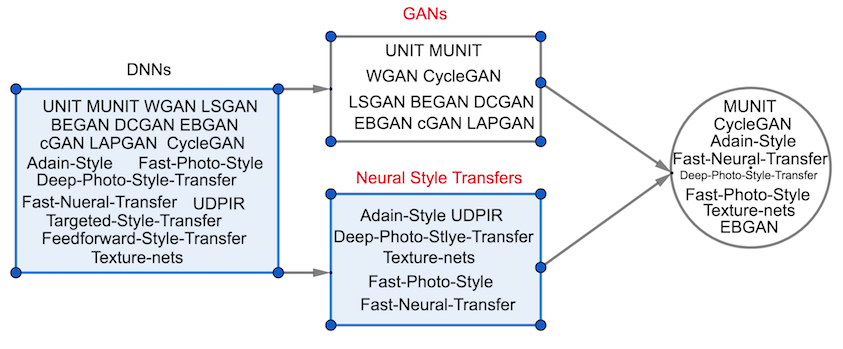
\includegraphics[width=0.9\textwidth]{filter}
    \caption{模型筛选过程}
    \label{fig:filtering}
\end{figure}

在有了足量的数据集后,基于DeepRoad的工作,我们首先选择实验的DNN模型大类是对抗生成网络\cite{GAN},因为其生成仿照数据的功能契合我们对于合成驾驶场景图片的需求,为了对目前所有的对抗生成网络技术能有一个综合的认识,我们首先参考了文献\cite{gan-survey},其中给出了目前学术界最为主流、为人熟知的几个模型算法:cGAN\cite{cGAN},DCGAN\cite{dcgan},LAPGAN\cite{LAPGAN}和EBGAN\cite{ebgan}等。我们一次对上述算法模型都进行了实验,但是其中dcGAN和LAPGAN在论文中没有开放其实验源码,且DCGAN在我们已有的路况图片数据集上的实验效果十分不理想,于是在实验初期我们排除了这几个模型。

在实验过上述模型后,我们通过Google搜索引擎,论文引用等途径陆续又发现了对抗生成网络中可以实现图像合成的几个模型,其中有一类是属于图片合成的输入需要有一张大致的纹理图,即给定一张样本纹理图和一组待转换的原图,输出为纹理跟输入纹理图一致的一组合成图,很明显这根我们的实验目的不匹配,因此被排除了。这一大类的模型有:MGAN\cite{MGAN},SGAN\cite{SGAN}和PSGAN\cite{PSGAN}。

另一类是属于图像填充功能,即跟据图片整体图像风格自动补充图片中因各种原因产生的空缺漏洞,这在计算机图形学和计算机视觉一致是个热门的研究领域,传统的方法是使用像素的复制和插值等数学方法来填充。对抗生成网络则提出了不一样的方法,通过学习大量同类的完整图片来实现图片的自动填充功能,比如文献\cite{GAN-inpaiting}提出的内容编码器方法。但由于这类模型跟我们图像风格转换的需求不匹配,因此没有做更深入的调研。

类似的,还有专门为人脸图像合成的模型,比如Age-cGAN\cite{Age-cGAN}。该类模型一般由一个编码器和条件对抗生成网络组成,其中编码器$E$将人脸图像$x$映射到一个潜在向量$z$中,条件生成器$G$在将潜在向量$z$和条件年龄变量$c$映射到合成一张新的人脸图。为了验证该类模型效果,我们首先在人脸数据上对这类模型进行了实验,成功复现了人脸自动合成的功能,但其在自动驾驶场景转换上的效果却很差。这可能是因为模型中使用的条件年龄变量对于自动驾驶场景图像的生成没有对应的参照物,因此这一类模型实验数据我们没有作最后的统计。


图\ref{fig:filtering}是我们对对抗生成网络模型筛选的大概历程,前后我们实验过的模型11个,最后统计实验数据统计总结的模型个数有4个,即UNIT\cite{UNIT},MUINT\cite{MUNIT},CycleGAN\cite{CycleGAN}和EBGAN\cite{ebgan}。

在选择对抗生成网络模型的过程中,除了模型本身的合成效果特点外,最大的困难是合适的数据集收集。在实验的初期我们就注意到大多数的对抗生成网络模型的训练都对其训练数据集有较为严格的要求,即需要训练集中的内容图片集和风格图像集尽可能的接近。

在调研了深度学习技术重点对抗生成网络大类后,我们重点参考了文献\cite{nst-survey},了解到目前能够实现图像转换技术的深度学习框架比较流行的还有一类叫做图像风格转换技术的框架,顺着文献的分类我们对立面提到的模型都实验了一遍。最开始我们选取的是比较有代表性的Fast Neural Transfer进行了实验,最终结果差强人意。由于正如文献中提到的,图像风格转换技术最初是为人工合成艺术作品而产生的一项深度学习技术,在我们对这类技术模型实验的过程中发现大多数模型实验的结果虽然可以实现图像的风格转换,但都太艺术化了,距真实场景的图片出入太大,所以大部分的模型的实验结果我们最后都排除在了统计范围内,最后作为数据统计的模型有:Adin-Style\cite{adain},Deep Photo Style Transfer\cite{dpst},Fast Photo Style\cite{fps},Fast Neural Transfer\cite{FNT}和Texture Nets\cite{texture-nets}。

% TODO 插入图片

以上是我们对实验模型筛选的大致历程,下面简单的介绍一下对抗生成网络的背景以及选择的对应模型。

\subsection{对抗生成网络大类}[Generative Adversarial Network Class]

对抗生成网络\cite{GAN}首先由Ian J. Goodfellow等人提出,它的本质是模拟真实数据源的概率分布。其基本框架有两个神经网络组成:生成模型网络和判别模型网络,其中判别模型负责学习区分数据是否来自真实数据分布,而生成模型可以想象成一个制造伪币的团伙,试图产生能够通过货币监测的钞票,判别模型正是这个对抗游戏中的警察,试图甄别出货币中的假钞。整个对抗生成网络模型的训练过程就是对抗模型和生成模型的训练竞赛,整个训练过程直到判别模型再也区分不出数据是来自真实数据分布还是生成模型伪造的数据为止。

训练过程中,对抗模型一般使用向后传播算法,而判别模型一般使用向前传播算法。其中判别模型为了通过数据$x$学习生成器的数据分布$p_g$,可以基于输入的噪声数据定义一个先验概率$p_z(z)$,然后将整个数据空间表示为$G(Z;\theta_g)$,这里的$G$是一个参数为$\theta$的多层神经网络可微函数。再定义一个输出为一个单向量的多层神经元网络$D(x;\theta_d)$,其中$D(x)$表示数据$x$来自真实数据而非$p_g$的概率。我们训练$D$直到我们对所有数据正确标记其是否来自判别器的概率最大为止。同时也训练$G$来最小化$\log(1-D(G(z)))$。上述可总结成下面的公式:
\begin{equation}
    \label{eq:gan}
    \min_G\max_DV(D,G)=\xi_{x\sim p_{data}(x)}[\log D(x)]+\xi_{z\sim p_z(z)}[\log(1-D(z))]
\end{equation}
实际训练过程中,等式\eqref{eq:gan}中的生成器$G$可能会出现梯度消失的问题,但由于本文章不是对对抗生成网络算法的研究,所以就不在此展开了。实验过程中为了保持尽量跟框架作者实现的效果性能一致,我们只选取了提供了源代码的框架进行了实验。

% TODO: confirm this
\textbf{统一说明},本文后续所有的实验均是在64位Ubuntu 16.04.6 LTS操作系统,8核GTX 1080ti-GPU硬件环境下进行的。以下介绍在本次实证研究中所有实验过用于图像风格转换的深度学习模型。

\subsubsection{cGAN}

\textbf{cGAN.}\cite{cGAN}\quad 对抗生成网络一般有两个对抗模型组成:一个可以捕捉到真实数据分布的生成模型$G$和一个能够计算样本来自训练数据集而不是$G$的概率的模型$D$。$D$和$G$都是非线性映射函数,比如多层感知器网络。如果生成器和判别器都限定于一些额外信息$y$上,则对抗生成网络可以被拓展成一个条件模型。其中$y$可以使任意类型的辅助信息,比如来自其他模型的数据或标记。cGAN通过将数据信息$y$送入判别器和生成器中作为额外的输入层来实现条件限制。在生成器中先验噪声输入$p_z(z)$和$y$被混合在联合隐藏层中,在判别器中$x$和$y$代表判别函数的输入,cGAN的目标函数可以表示为:
\begin{gather}
    min_G max_D V(D,G)=\mathbb{E}_{\x\sim p_{data}(x)}[\log D(x|y)]+\mathbb{E}_{z\sim p_z(z)}[\log(1-D(G(z|y)))]
\end{gather}

因为文献中\cite{cGAN}主要对MNIST\cite{mnist}数据集进行了数字模拟合成,在已有的路况图像数据集上实验的结果很不理想,且文献中提供的代码对数据集的要求也与一般的模型输入不一样,需要额外的处理,因而我们放弃了在该模型上的进一步实验与数据统计。 

\begin{figure}[h]
    \centering
    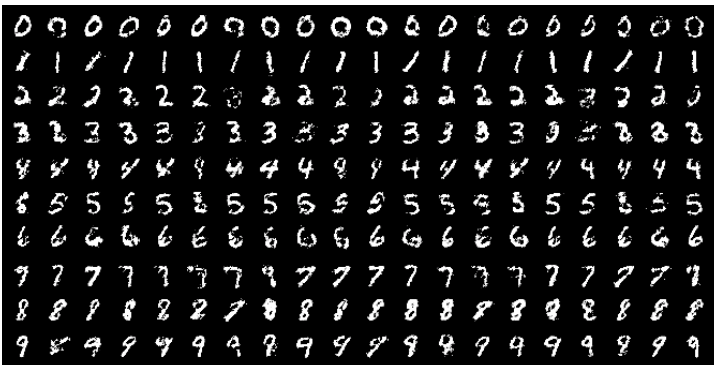
\includegraphics[width=.65\textwidth]{results/cgan}
    \caption{cGAN在MNIST数据集上的数字合成图片样例}
\end{figure}

\subsubsection{DCGAN}[DCGAN]

\textbf{DCGAN.}\cite{dcgan}\quad 是一个深度卷积对抗生成网络,其生成器和判别器使用的是限制卷积网络,主要的架构特点有:(1)用多步卷积和分布卷积层代替了所有的池化层(pooling layer);(2)使用了批量统一化层(batch normalization layer);(3)去掉了所有的全连接层;(4)在生成器中,使用$\tan{h}$作为输出层的激活函数,ReLU函数作为其它层的激活函数;(5)判别器中,所有层的激活函数都使用LeakyReLU函数。除此之外该算法结构中,所有正定空间池化函数都换成了多步卷积函数,这样可以使网络网络学习到整个图像空间的采样。

DCGAN主要目的是找到一个方法能够对图像进行特征重建及特征提取。DCGAN在其卷积神经网络的拓扑结构内提出了一套限制,使得该模型能够几乎在任何参数设置里都能够尽快的训练收敛。相较其他的对抗生成网络模型,DCGAN的主要优点是其稳定的网络结构和较快的训练收敛速度。DCGAN的作者将该模型在CIFAR-10\cite{cifar10}数据集上做了一次实证研究,结果也验证了DCGAN较其他GAN模型能够更快的学习到图像的特征。

虽然DCGAN的作者将其运用在人脸合成与转换上相当成功,但我们后来将其训练集换成了Udacity的自动驾驶路况数据集以及youtube上爬取的数据,实验结果样本图如下图\ref{dcgan_example}所示,效果却不理想。

\begin{figure}[h]
    \centering
    \subfigure[DCGAN在人脸图像合成的效果样例图]{
        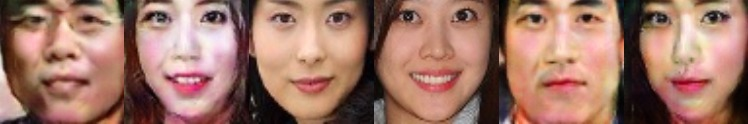
\includegraphics[width=0.75\textwidth]{dcgan_example}
    }
    \subfigure[DCGAN在自动驾驶数据集上的效果样例图]{
        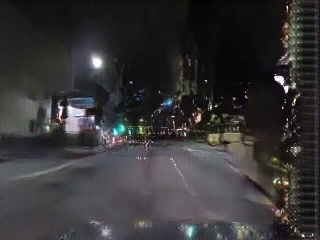
\includegraphics[width=0.4\textwidth]{results/dcgan_night}
        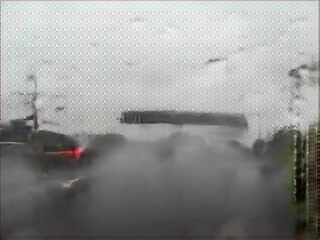
\includegraphics[width=0.4\textwidth]{results/dcgan_rain}
    }
    \caption{}
    \label{dcgan_example}
\end{figure}

实验代码使用的是\cite{dcgan}论文中给出的代码,其中主要参数配置如下

\begin{lstlisting}[basicstyle=\small]
    --bathSize     200          // 批量实验数据大小
    --imageSize    180, 320     // 设置图像尺寸大小
    --nz           20           // z向量
    --niter        10000        // 训练的次数
    --lr           0.0002       // Learning rate
    --cuda                      // 在cuda库上训练
\end{lstlisting}

由于DCGAN在驾驶路况图片上的合成效果很差,于是我们放弃了对该框架进一步的实验结果数据统计与总结。

\subsubsection{LAPGAN}

\newmodel{LAPGAN} 该模型利用了图像的多尺度结构,针对每个尺度构建了一系列的生成模型,每个模型都在特定尺度的拉普拉斯算子\cite{lapcode}上捕获到了图像的结构特征。这种方法将原来的图像转换问题成功地分解成了一系列可控状态,对于每个状态都可以使用一般的对抗生成网络结构训练一个基于卷积神经网络的生成模型。

在视觉应用,比如目标分类中的判别模型中,使用深度学习的方法常常十分有效。但是对于生成模型,尽管进行了相当多的研究\cite{lapgan1}\cite{lapgan2}\cite{lapgan3},却往往没有取得同等级别的成功。基于这样的问题,LAPGAN提出了模型在生成模型的训练效果上取得了巨大的改进。模型中使用的拉普拉斯算子是由一组图像的线性非可逆表征组成。具体的,使$d(\cdot)$表示模糊化$i\times j$图像$I$的缩减采样算子,则$d(I)$表示尺度为$j/2\times l/2$的新图像。类似地,令$u(\cdot)$表示将图像$I$光滑化的升采样算子,$u(I)$表示尺度为$2j\times 2j$的新图像。算法中首先构建一个高斯拉普拉斯算子$\mathbb{G}(I)=[I_0,I_1,\dots,I_K]$,这里的$I_0=I$和$I_k$表示$d(\cdot)$对$I$的$k$次重复操作。$K$是该算子中的层数。拉普拉斯网络中每一层$k$的系数$h_k$都是由邻近层中的距离计算构成,对图像使用算子$u(\cdot)$进行升采样操作:
\begin{gather}
    h_k=\mathbb{L}_k(I)=\mathbb{G}(I)-u(\mathbb{G}_{k+1}(I))=I_k-u(I_{k+1})
\end{gather}
每层都很直观的包含了特定尺度的图像结构信息。拉普拉斯算子$h_k$的最终结构是一张不同的图像。以此为基础可成功的重构一张新图像。

该算法文献\cite{LAPGAN}中在CIFAR10数据集上进行了图像转换实验,但实验的代码没有进行开源,因此我们暂时性的忽略了该算法的实验。将来该算法代码开源后我们会针对该算法进行补充实验和数据统计。 

% wc ~ 1200

\subsubsection{CycleGAN}[CycleGAN]

\textbf{CycleGAN.}\cite{CycleGAN}\quad 该模型的本质是学习不同图片类(比如晴天和雨天)的数据分布映射函数。给定两个不同类的数据集$X$和$Y$以及训练样本集$\{x_i\}_{x=1}^N, \{y_j\}_{j=1}^M$,其中$x_i\in X, y_j\in Y$。将数据分布记为$x\sim p_{data}(x), y\sim p_{data}(y)$。如图\ref{lable-cyclgan}所示,CycleGAN包含两个映射函数$G: X\to Y$和$F: Y\to X$,其次,CycleGAN还引进了两个判别器$D_X$和$D_Y$,其中$D_X$的目标是区分图像集$\{x\}$和转换的图像集$\{F(y)\}$,同样的,$D_Y$的目标是区分图像集$\{y\}$和$\{G(x)\}$。最终模型的训练目标是得到两个损失函数:(i)对抗损失函数,可以将合成的图像数据分布匹配对应到目标类的数据分布上;(ii)循环一致损失函数,阻止之前学习到的两个映射函数$G$和$F$彼此相矛盾。

\begin{figure}[h]
    \centering
    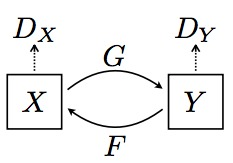
\includegraphics[width=.35\textwidth]{cyclegan_1}
    \caption{CycleGAN}
    \label{lable-cyclgan} 
\end{figure}

CycleGAN将对抗损失应用到了两个映射函数上,对于映射函数$G:X\to Y$和他的判别器$D_Y$,可以将其目标函数表示为
\begin{equation}
\begin{aligned}
    \label{eq:2}
    L_{GAN}(G,D_Y,X,Y)= & \xi_{y\sim p_{data}(y)}[\log D_Y(y)] + \\
    & \xi_{x\sim p_{data}(x)}[\log (1-D_Y(G(x)))]
\end{aligned}
\end{equation}

这里的$G$试图产生类似于类$Y$的图像集$G(x)$,然而$D_Y$的目标是区分转换的图像$G(x)$和真实的图像数据$y$。$G$旨在与对抗器$D$竞争最小化该目标函数。

\begin{figure}[b]
    \centering
    \subfigure[原始图片]{
        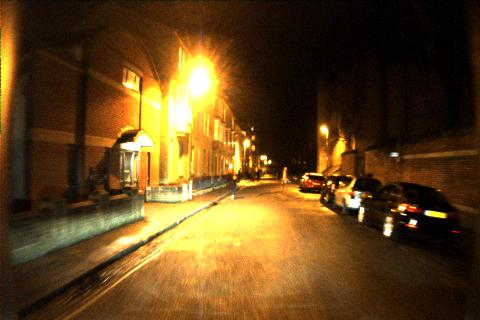
\includegraphics[width=0.3\textwidth]{results/cyclegan-input}
    }
    \subfigure[白天场景]{
        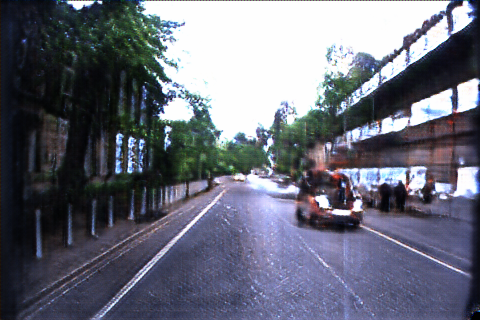
\includegraphics[width=0.3\textwidth]{results/cyclegan-sun}
    }
    \subfigure[黑天场景]{
        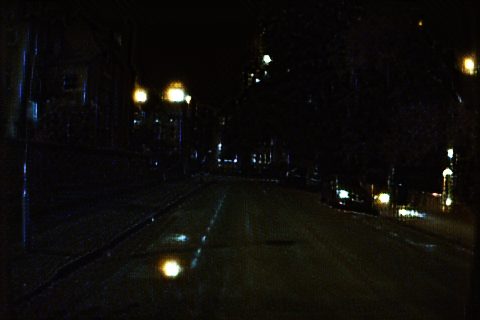
\includegraphics[width=0.3\textwidth]{results/cyclegan-night}
    }
    \subfigure[官方样例-1]{
        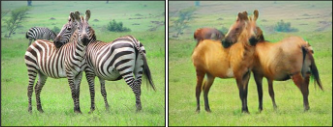
\includegraphics[width=0.45\textwidth]{cyclegan_o_1}
    }
    \subfigure[官方样例-2]{
        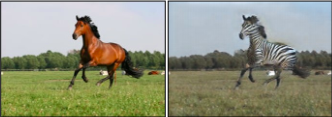
\includegraphics[width=0.45\textwidth]{cyclegan_o_2}
    }
    \caption{CycleGAN实验样例图以及官方图像转换样例图}
    \label{fig:cyclegan}
\end{figure}

对抗器理论上可以训练出可以输出和目标类$Y$与$X$分布完全相同的数据的映射函数$G$和$F$,但是如果网络的体积足够大,可以将相同的输入图片集映射到目标图片类的任意图像子集里。因此,单靠对抗损失函数无法保证学习到了映射函数能将单张输入图片$x_i$映射到理想的输出$y_i$。为了进一步减小可能的映射函数空间,CycleGAN提出循环一致映射函数,即对于来自类$X$的每张图像,对应的图像转换循环应该能够将$x$转换成原始图片,即\textit{向前循环一致}。上述的循环一致损失函数可以表示为:
\begin{equation}
\begin{aligned}
    \label{eq:3}
    L_{cyc}(G,F)= & \xi_{x\sim p_{data}(x)}[||F(G(x))-x||_1] + \\
    & \xi_{y\sim p_{data}(y)}[||G(F(y))-y||_1]
\end{aligned}
\end{equation}

综合等式\ref{eq:2}和等式\ref{eq:3}我们可以得到总的目标函数:
\begin{equation}
\begin{aligned}
    L(G, F, D_X, D_Y) = & L_{GAN}(G,D_Y, X, Y) \\
    & + L_{GAN}(F,D_X, Y, X) \\
    & + \lambda L_{cyc}(G, F)
\end{aligned}
\end{equation}
这里的$\lambda$控制着两个目标的相对重要性。

CycleGAN对于内容图片通训练图片不相似的情况转换合成效果并不好,常常会造成合成图的语义不明确。它通常适合于颜色和图像纹理转换的情形,对于合成图有内容变化的情形,CycleGAN合成图的效果会比较差,其作者分析其中的原因可能是因为常常会为了提高图像信息变化更高效而裁减生成器的网络复杂度,这使得CycleGAN对于内容改变的性能变差。文献\cite{CycleGAN}中也提到了CycleGAN对于一组不相似的图片训练出来的模型效果较一组相近训练数据集模型效果会差很多,并且很难消除这两者间的差异。

图\ref{fig:cyclegan}是我们将CycleGAN运用在我们的数据集上,进行了晚上到白天以及黑天场景转换的实验结果样本图以及CycleGAN在其官方给定的数据集上的图像转换效果。 

% wc ~ 800

\subsubsection{WGAN}

\newmodel{WGAN} 该算法相较其他的GAN模型的主要改进依然是提升了模型训练的稳定性和收敛速度。WGAN提出了Earth-Mover距离,并证明了该距离比其他的距离尺度指标能产生更好的梯度,从而提升训练速度。此外它关于判别器网络还去掉了对应了sigmoid层,在对抗损失函数中去掉了log函数,有效地避免的类似模型塌缩等问题。理论上图像合成的效果要好于DCGAN。

因为WGAN文献中只给出了算法的核心思想,没有给出实验源码。我们参考文献中提供的算法,实现了WGAN的图像转换代码,但是在路况图像数据集上的实验结果十分不理想,合成的图像与原图像在语义上相差甚远,我们推测可能是算法实现没有成功导致,最终我们没有将该实验结果纳入最后的实验数据总结和统计中。

\subsubsection{MUNIT}[MUNIT]

\textbf{MUNIT.}\cite{MUNIT}\quad MUNIT是基于UNIT\cite{UNIT}工作的进一步优化。它主要针对的问题时候多类图像间的图像转换问题。比如一个冬天的道路场景在夏天可能会依天气、时间等因素的不同而有很多种不同的外在形式。CycleGAN希望其生成器能够包含一个场景中尽可能多的表征空间。

除此之外它提出了一个可以解决多模型图片到图片转换问题的框架。它对于图像转换问题提出了几个假设:图片的潜在空间(latent space)可以被分解成内容空间和样式空间。基于上一个假设又提出了不同域类的图片共享一个类似的内容空间,但样式空间不一致。为了将一张图片转换成目标域类,MUNIT提出可以将图片的内容码与目标域类样式码空间的一个随机样式码重组。这里的内容码代表了在图片转换过程中应该被保留的信息元,而状态码则代表了不包含在输入图片中还剩下的变量元。通过采样不同的状态码,MUNIT模型能够产生多样,多模型的输出。以上严格的数学定义如下:

\begin{figure}[t]
    \centering
    \subfigure[原始图片]{
        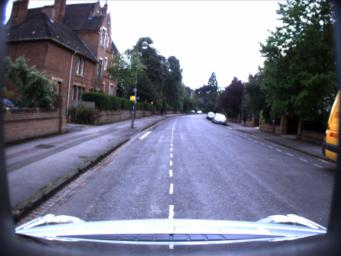
\includegraphics[width=.3\textwidth]{results/munit}
    }
    \subfigure[雪天场景1]{
        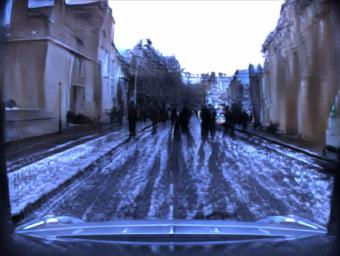
\includegraphics[width=.3\textwidth]{results/munit_winter}
    }
    \subfigure[雪天场景2]{
        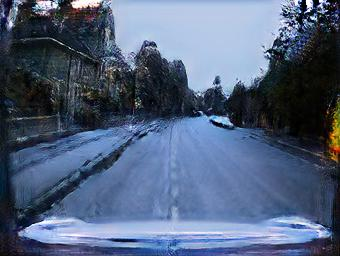
\includegraphics[width=.3\textwidth]{results/munit_winter2}
    }
    \subfigure[官方实验样例图]{
        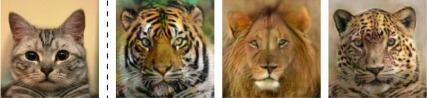
\includegraphics[width=0.8\textwidth]{munit_o_1}
    }
    \caption{MUNIT实验样例图}
    \label{fig:munit}
\end{figure}

假定$x_1\in \chi_1$和$x_2\in \chi_2$是来自两个图片域类的图片集,给定来自两个不同边缘分布$p(x_1)$和$p(x_2)$的样本图片集,但不知道联合分布$p(x_1, x_2)$。MUNIT的目的是利用学习到的图片到图片转换模型$p(x_{1\to 2}|x_1)$和$p(x_{2\to 1}|x_2)$来预测两个边缘分布$p(x_1|x_2)$和$p(x_2|x_1)$,这里的$x_{1\to 2}$是由将$x_1$转换成$x_2$产生的一个样本输出。一般来说,$p(x_1|x_2)$和$p(x_2|x_1)$通常是十分复杂且多模型分布,为了简化这两个边缘分布,MUNIT提出了\textit{部分共享潜在空间假设}。即假设每张图片$x_i\in \chi_i$都是由两种码,内容码和样式码,组成,其中内容码$c\in C$由两个类域共享,而样式码$s_i\in S_i$则是每个域类图片所特有的。换句话说,一组来自联合分布的对应的图片$(x_1, x_2)$是由$x_!=G_1^*(c,s_1)$和$x_2=G_2^*(c, s_2)$生成的,这里的$c,s_1,s_2$都是来自鲜艳分布,$G_1^*,G_2^*$是实际的生成器。进一步假设$G_1^*$和$G_2^*$是确定性函数,且有反解码器$E_1^*=(G_1^*)^{-1}$和$E_2^*=(G_2^*)^{-1}$。MUNIT的目的是利用神经网络学习实际的生成器以及编码函数。它使用了两个重建的目标函数:给定来自数据分布的图像样本,在编码和解码后我们能够重建它:
\begin{gather}
    L_{recon}^{x_1}=E_{x_1\sim o(x_1)}[||G_1(E_1^c(x_1), E_1^s(x_1))-x_1||_1] 
\end{gather}

给定在转换时的样式和内容码,我们也应该能够在解码和编码后重建图像:
\begin{equation}
    \begin{aligned}
        L_{recon}^{c_1}= & E_{c_1\sim p(c_1), s_2\sim q(s_2)}[||E_2^c(G_2(c_1,s_2))-c_1||_1] \\
    L_{recon}^{s_2}= & E_{c_1\sim p(c_1), s_2\sim q(s_2)}[||E_2^s(G_2(c_1, s_2))-s_2||_1]
    \end{aligned}
\end{equation}

结合以上公式,MUNIT的总的损失函数可以由下面的公式表示:
\begin{equation}
\begin{aligned}
    \min_{E_1,E_2,G_1,G_2}\max_{D_1,D_2}L(E_1,E_2,G_1,G_2,D_1,D_2)=L_{GAN}^{x_1}_L_{GAN}^{x_2}+\\
\lambda_x(L_{recon}^{x_1}+L_{recon}^{x_2})+\lambda_c(L_{recon}^{c_1}+L_{recon}^{c_2})+\lambda_s(L_{recon}^{s_1}+L_{recon}^{s_2})
\end{aligned}
\end{equation}

总体来说,MUNIT是一个多模型无监督图像到图像的转换框架。在目前的无监督方法中图像转换质量和转换图像的种类都更好更多。最后我们使用了MUNIT提供的代码,进行了晴天路况图和雪天场景的转换,主要的优化配置参数如下,最终的实验结果样例及MUNIT官方实验样例图参考图\ref{fig:munit}:

\begin{lstlisting}[basicstyle=\small, caption={MUNIT主要优化参数配置}, captionpos=b]
    max_iter: 1000000             # maximum number of training iterations
    batch_size: 1                 # batch size
    weight_decay: 0.0001          # weight decay
    beta1: 0.5                    # Adam parameter
    beta2: 0.999                  # Adam parameter
    init: kaiming                 # initialization [gaussian/kaiming/xavier/orthogonal]
    lr: 0.0001                    # initial learning rate
    lr_policy: step               # learning rate scheduler
    step_size: 100000             # how often to decay learning rate
    gamma: 0.5                    # how much to decay learning rate
    gan_w: 1                      # weight of adversarial loss
    recon_x_w: 10                 # weight of image reconstruction loss
    recon_s_w: 1                  # weight of style reconstruction loss
    recon_c_w: 1                  # weight of content reconstruction loss
    recon_x_cyc_w: 10             # weight of explicit style augmented cycle consistency loss
    vgg_w: 0                      # weight of domain-invariant perceptual loss
\end{lstlisting}

\subsubsection[EBGAN]{EBGAN}

\begin{figure}[b]
    \centering
    \subfigure[原始图片]{
        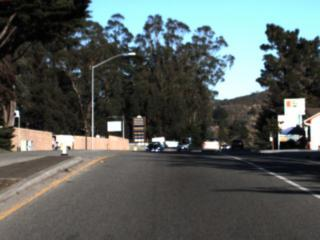
\includegraphics[width=.45\textwidth]{results/ebgan-input}
    }
    \subfigure[雨天场景]{
        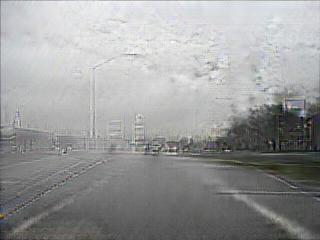
\includegraphics[width=.45\textwidth]{results/ebgan-rain}
    }
    \subfigure[官方人脸合成样例图]{
        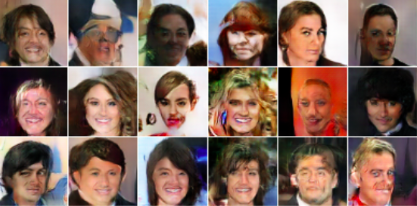
\includegraphics[width=0.8\textwidth]{ebgan_o_1}
    }
    \caption{EBGAN实验样例图}
    \label{fig:ebgan}
\end{figure}

\textbf{EBGAN.}\cite{ebgan}\quad 的核心思想是将判别器视为一个能量函数而不是通常的概率函数。它构建了一个函数能将输入空间中的每个点映射成为一个单标量,并且提出了对抗生成模型训练的一个基于能量表达的公式。由判别器计算出来的能量函数可以被视作生成器的可训练代价函数。虽然可以将能量函数通过Gibbs分布转换成概率函数,但是基于它提出的基于能量形式的对抗生成网络由于缺少归一化,从而使我们在判别器的架构和训练过程中有了更多的选择。EBGAN的学习构成是由数据驱动,定型能量函数是的好的模型参数配置获得低能量而不好的配置参数获得高能量。这种训练书序监督学习的一种:对于每训练集中的每个$X$,一种$(X,Y)$的能量只有当$Y$是好的配置参数时才会获得低能量,反之获得高能量。下面简单阐述一下EBGAN的基本原理。

将$p_{data}$视作产生真实数据集分布的概率密度函数,生成器$G$训练生成赝本数据$G(z)$。为了定义能量函数,判别器的输出通过一个目标泛函算子进行转换,将低能量视为真实样本数据,而高能量则为合成的伪数据。跟一般的对抗生成网络一样,EBGAN也使用了两个不同的损失函数来分别训练生成器和判别器。

给定一个正边缘分布函数$m$,一个数据样本$x$和一个生成样本$G(z)$,判别器损失函数$L_D$和生成器损失函数$L_G$可以定义为以下:
\begin{equation}
    \begin{align*}
    L_D(x, z) = & D(x) + [m - D(G(z))] \\
    L_G(z) = & D(G(z))
    \end{align*}
\end{equation}

给定一个生成器$G$,$p_G$为$G(z)$的密度分布,这里$z\sim p_z$。换句话说,$p_G$是由$G$产生的样本的概率密度函数。定义$V(G,D)=\int_{x,z}L_D(x,z)p_{data}(x)p_z(z)dxdz$和$U(G,D)=\int_zL_G(z)p_z(z)dz$,训练中判别器来最小化$V$值,生成器最小化$U$值。该系统的纳什均衡是一组满足一下条件的一对$(G^*,D^*)$:
\begin{equation}
    \begin{aligned}
        V(G^*,D^*) \leq V(G^*,D) \quad\quad \forall D \\
        U(G^*,D^*) \leq U(G,D^*) \quad\quad \forall G 
    \end{aligned}
\end{equation}

EBGAN打通了两类不同的非监督学习方法:对抗生成网络和自动编码器,并且从基于能量的角度重新采用对抗生成网络的结构并定义新的训练损失函数。对于高分辨率图片,相较其他类的对抗生成网络技术,EBGAN的模型训练有更快的收敛速度,且合成图片也有更好的合成效果。

我们在已有的数据集上使用了tensorflow实现的EBGAN代码\cite{ebgan-github},实现了晴天路况到雨天场景的转换,图\ref{fig:ebgan}是实验结果样例图及官方人脸合成实验样例图。

\subsubsection{LSGAN}

\newmodel{LSGAN} 一般的GAN模型都使用sigmoid交差熵作为判别器的损失函数,使用这类损失函数都存在一个问题,就是在模型训练过程中很容易出现梯度消失的问题,导致最后合成的数据离真实数据分布相差较大。针对这一问题LSGAN提出使用最小方差函数最为判别器的损失函数,因为最小方差损失函数能够使判别器对接近判断边界的伪数据做出惩罚。除此之外,LSGAN还能提高模型训练过程的稳定性。文献\cite{LSGAN}提到实验结果显示LSGAN合成的数据别一般的GAN合成输数据更接近与真实数据分布。该算法的目标损失函数为:
\begin{equation}
\begin{aligned}
    & \min_D V_{LSGAN}(D)=\frac{1}{2}\mathbb{E}_{x\sim p_{data}(x)}[(D(x)-b)^2]+\frac{1}{2}\mathb{E}_{z\sim o_z(z)}[(D(G(z))-z)^2] \\
    & \min_G V_{LSGAN}(G)=\frac{1}{2}\mathb{E}_{z\sim p_z{z}}[(D(G(z))-c)^2]
\end{aligned}
\end{equation}

下图\ref{fig:lsgan}是LSGAN和一般的GAN图像合成样本的对比图。

\begin{figure}[h]
    \centering
    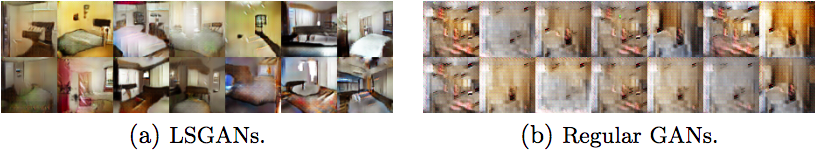
\includegraphics[width=\textwidth]{results/lsgan}
    \caption{LSGAN合成图像对比图}
    \label{fig:lsgan}
\end{figure}

由于文献中的实验代码没有开源,于是我们利用DCGAN的源码将其判别器的损失函数改为文献中提到了最小方差函数,但是最后的实验结果跟DCGAN的实验结果相差不大。基于较差的实验结果我们舍弃了该模型实验结果的数据统计和总结。

\subsubsection{MGAN}

\newmodel{MGAN} 大部分用于图像合成的对抗生成网络技术都是使用马尔可夫随机场来处理图像复杂的限制特征,这些马尔可夫随机场也通常是使用像素块的统计数据来表征图像的。这类技术通常分为两类:合成完整图像的全图像模型和只合成图像纹理层的马尔科夫模型。MGAN主要的改进是提升了深度马尔科夫模型对纹理合成的效率与质量。文献\cite{MGAN}中使用对抗训练\cite{adtrain}算法训练卷积神经网络,这样可以维持与原图几乎不变的图片质量,同时极大地提升了图像合成速度,40ms内合成一张$512\times 512$图像,其中硬件条件为TitanX GPU。

因为MGAN的优化主要针对人脸合成类别,且与传统的图像合成技术类似,合成图片具有明显的艺术风格。我们利用文献中提供的代码\cite{git:mgan}在我们的路况图像数据集上实验结果跟文献中的实验结果一致,具有太明显的艺术风格,因而在最后的实验数据统计和总结环节我们没有考虑该模型的实验数据。下图\ref{fig:mag}为MGAN的实验数据样例图。

\begin{figure}[h] 
    \centering
    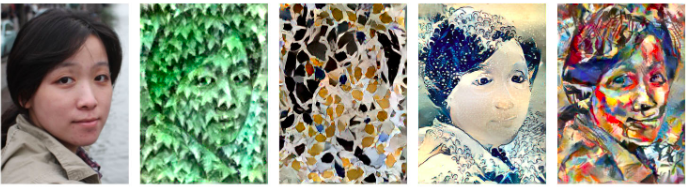
\includegraphics[width=.9\textwidth]{results/mgan}
    \caption{MGAN实验样例图}
    \label{fig:mag}
\end{figure}

\subsubsection{BEGAN}

\newmodel{BEGAN}  该模型跟EBGAN\cite{ebgan}一样使用了自动编码器作为判别器。虽然一般典型的对抗生成网络模型都直接匹配数据分布,但是BEGAN的目的是利用从Wasserstein距离中推到出了损失函数,来匹配自动编码器损失值。分布。实际的模型算法中,使用了一个典型的对抗生成网络目标函数,加上一个额外的平衡判别器和生成器的平衡因子。这样使得模型的训练更加容易。文献\cite{BEGAN}中对于自动编码器使用的损失函数$\mathb{L}:\mathbb{R}^{N_x}\to \mathbb{R}^+$为:
\begin{align}
    \mathb{L}(v) = |v-D(v)|^\eta where \begin{cases}
        D: \mathbb{R}^{N_x}\to \mathbb{R}^{N_x} \quad  \\
        \eta \in \{1,2\} \quad  \\
        v \in \mathbb{R}^{N_x} 
    \end{cases}
\end{align}

模型总体的目标函数可表示为:

\begin{align}
    \begin{cases}
        L_D = L(x) - k_t\cdotL(G(z_D)) & for \quad \theta_D \\
        L_G = L(G(z_G)) & for \quad \theta_G \\
        k_{t+1} = k_t + \lambda_k(\gammaL(x)-L(G(z_G))) 
    \end{cases}  
\end{align}

我们参照文献中的代码实现了WGAN的人脸图像合成,但将数据源换成我们的路况图像数据集后,程序出现了未知的BUG,导致最终的路况图像合成实验没能完成。下图\ref{fig:began}为BEGAN的人脸合成结果样例图。

\begin{figure}[h]
    \centering
    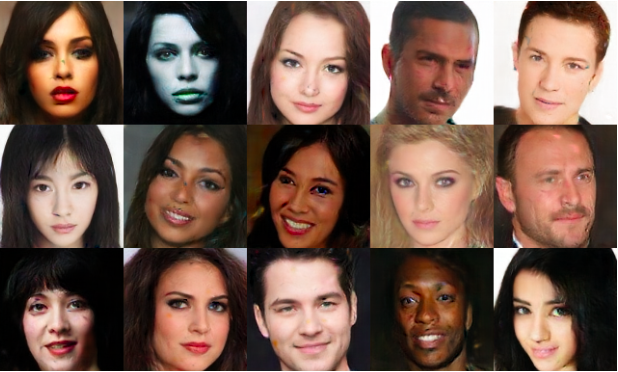
\includegraphics[width = .8\textwidth]{results/began}
    \caption{BEGAN人脸合成样例图}
    \label{fig:began}
\end{figure}

% wc ~ 1700

\subsection{图像风格转换大类}[Neural Style Transfer Class]

图像风格转换技术是受启发于近20年来卷及网络神经的发展,Gatys等人\cite{nst}提出利用卷积神经网络来复现一些著名的绘画风格。他提出利用神经元来实现将图像中的内容和风格分开和重组的功能。以物体识别中的卷积神经网络为例,其在训练过程中,会随着网络层数的增加,其神经元对图像表征能力也会随之增加。因此,随着网络结构层数的深入,输入图片也会被转换成比原始图中像素值更具表征性的神经元输出。于是Gatys提出可以直接从高特征层包含的信息重建图像。越高的网络层能够捕获更高级的图像语义信息。因此Gatys将高层中的特征表示看做图像的内容表征。

为了能将包含在网络结构中不同层间冬天图片信息可视化,文献\cite{nst}提出可以在一张白噪声图片上利用梯度下降算法来找到另一张可以匹配原始图片特征空间的图片。令$\overrightarrow{p}$和$\overrightarrow{x}$表示原始图片和合成图片。$P^l$和$F^l$分别表示它们在$l$层的表征。定义两个表征之间的方差损失为:
\begin{align}
    L_{content}(\overrightarrow{p},\overrightarrow{x},l)=\frac{1}{2}\sum_{i,j}(F_{ij}^l-P_{ij}^l)^2
\end{align}
该损失函数对应于$l$层激活函数的导数等于
\begin{align}
    \frac{\partial L_{content}}{\partial F_{ij}^l} = \begin{cases}
        (F^l-P^l)_{ij}  & if \quad F_{ij} > 0 \\
        0 & if \quad F_{ij}^l \lt 0
    \end{cases}
\end{align}

由此对用与图片$\vec{x}$的导数可以通过标准误差的向后传播算法计算得出,从而我们可以改变初始的随机图片$\vec{x}$直到在卷积层中某一层产生跟原始图$\vec{p}$表征一致的特征。

对于输入图像的风格表征,Gaatys利用原本用来捕获图像纹理信息的特征空间。该特征空间建立在网络层的过滤网之上。它由特征空间中不同层的过滤网之间的协方差组成,通过包含多层间的特征协方差,就可以获得一个静态、多尺度的输入图片表征值,该表征形式捕获了输入图像的纹理信息。

为了获得输入图片的风格表征形式,他们使用了一个原本用来获取图层信息的特征空间。该特征空间构建于神经网络的每一层过滤网之上。它由特征图谱各个部分的过滤网之间的协方差组成。通过引进多层网络之间的特征协方差,可以得到一个输入图片的一个静止、多尺度的能够包含图层信息的表征形式。再者,还可以通过构建一张匹配给定的输入图片的样式表达的图片来将建立在网络中不同层的样式特征空间信息可视化。为了合成拥有输入图片样式的图片,一般的图像风格转换技术会最小化来自一层网络的内容表征的白噪声图片与卷积网络层中输入图片的样式表征之间的距离。让$\overrightarrow{p}$表示合成照片,$\overrightarrow{a}$表示输入图片,则损失函数可以表示为:
\begin{align}
    L_{total}(\overrightarrow{p},\overrightarrow{a}, \overrightarrow{x})=
    \alpha L_{content}(\overrightarrow{p}, \overrightarrow{x}) +
    \beta L_{style}(\overrightarrow{a}, \overrightarrow{x})
\end{align}

这里的$\alpha$和$\beta$分别表示内容和样式在重建过程中的权重。一般地通俗来讲,Neural Style Transfer转换合成图片需要3张图片,即内容图片,风格图片(通常为艺术画等),及需要进行风格转换的输入图片。进行图像合成转换的原理即定义两个距离函数:$Lcontent$表示两张图片内容的差异,$Lstyle$表示两张图片就风格而已之间的差异。对于第三章输入图片,通过神经网络变换输入图片的像素值,使其内容同内容图片的距离最小化,风格同风格图片的距离最小化,最终的损失函数记为以上两个距离函数之和。 

下面我们参考了文献\cite{nst-survey},根据里面给出的分类抽取了具有代表性的几个模型进行了实验,实验平台跟之前的实验一致。

\subsubsection[AdaIN-style]{AdaIN-style}

\textbf{AdaIN-style.}\cite{adain}\quad AdaIN Style主要针对Gatys提出的Neural Style Transer算法中,模型的训练需要一个很慢的迭代优化算法,这大大延长了模型的训练时间,其限制了它在很多场景下的实用价值。因此AdaIN Style提出使用前向传播神经网络的快速逼近算法来加速图像风格转换技术。但是速度的提升也会导致网络限制在了固定的一套风格集中,而无法使用到任意的风格集中。针对以上问题AdaIN Style提出了可以实时转换任意风格的框架。

\begin{figure}[!hb]
    \centering
    \subfigure[]{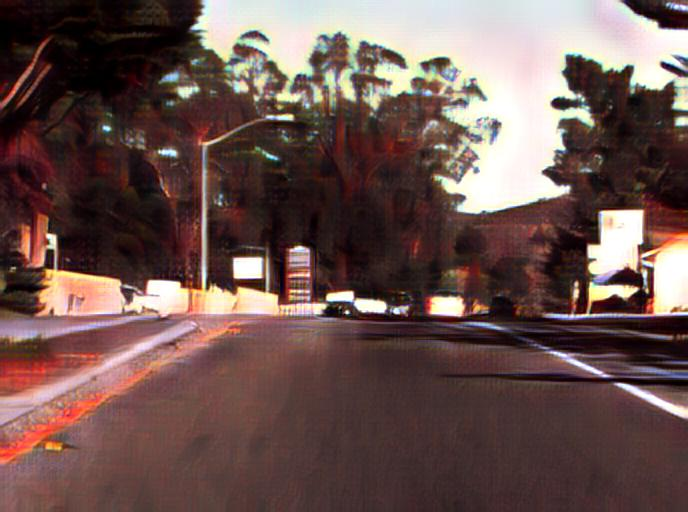
\includegraphics[width=.23\textwidth]{adin/adin1}}
    \subfigure[]{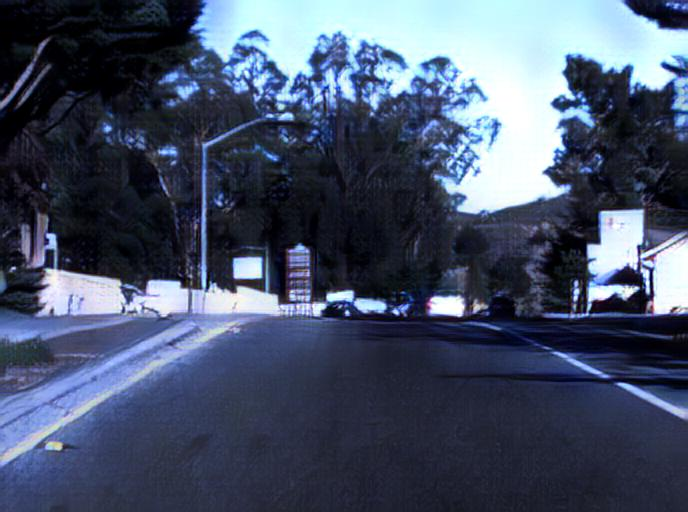
\includegraphics[width=.23\textwidth]{adin/adin2}}
    \subfigure[]{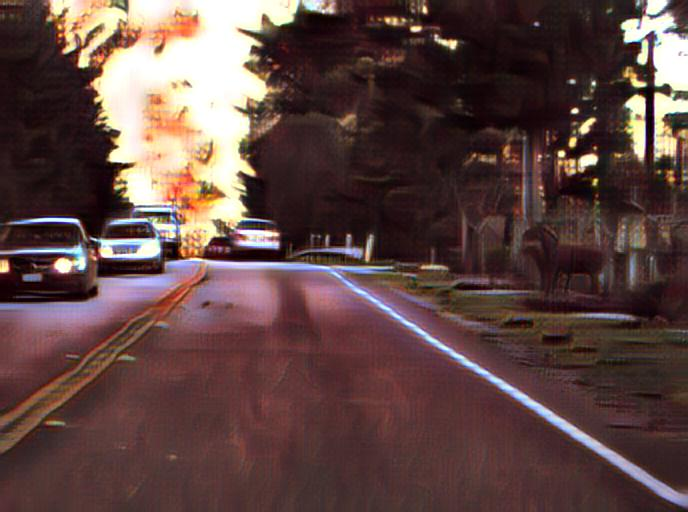
\includegraphics[width=.23\textwidth]{adin/adin3}}
    \subfigure[]{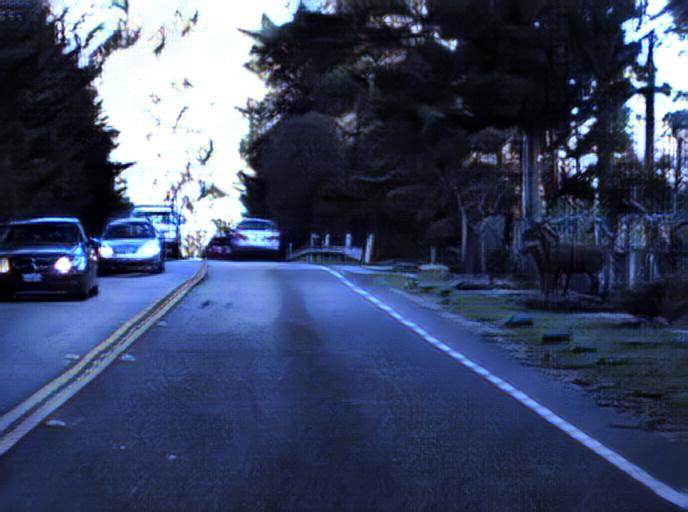
\includegraphics[width=.23\textwidth]{adin/adin4}}
    \subfigure[官方样例图]{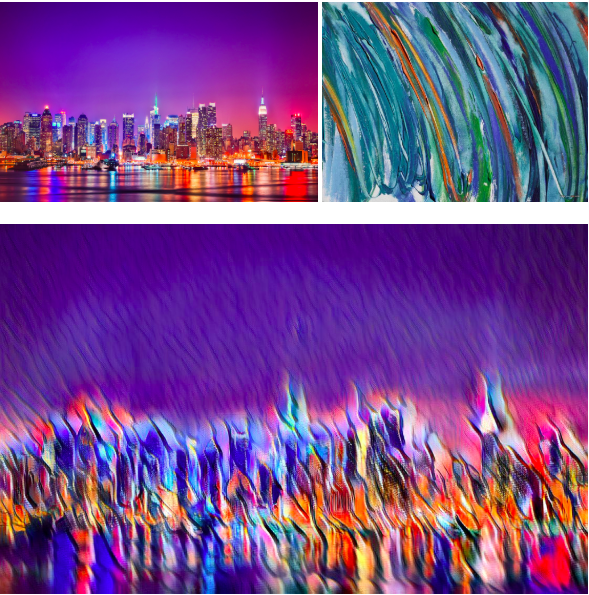
\includegraphics[width=.8\textwidth]{adin_o_1}}
    \caption{AdaIN实验结果样例图}
    \label{fig:adin}
\end{figure}

文献\cite{ioffe}提出批量正则化层极大的简化了向前传播网络的训练,AdaIN-style的模型结构也使用了批量正则化层,并且在次基础上通过将该层的激活函数改为单例正则,训练性能得到的巨大提升:
\begin{align}
    IN(x)=\gamma(\frac{x-\mu(x)}{\tau(x)})+\beta
\end{align}
与之前的批量正则层不同的是单例层在测试阶段不变,然而批量正则层通常会用总体统计数据替换掉批量神经元的均值。

除了学习仿射参数$\gamma$和$\beta$,另一个改进方式是为每一个样式$s$学习不同的参数$\gamma^*$和$\beta^*$:
\begin{align}
    CIN(x;s)=\gamma^*(\frac{x-\mu(x)}{\tau(x)})+\beta^*
\end{align}
训练过程中,样例图片和它的指数$s$被随机从一个固定的样例集合$s\in {1,2,\dots,S}(S=32)$选取。内容图片会被样式转换网络进行转换,该网络中对应的$\gamma^*$和$\beta^*$被用在条件单例正则层里。

总体来说,AdaIN通过转换特征统计量,特别是像素均值和方差,来实现特征空间的样式转换。除此之外,AdaIN Style加深了深度图像表征的理解。其与Gatys提出的Neural Style Transfer主要区别在于两者之间的优化过程和具体的优化函数的不同,AdaIN Style的网络结构也可以多变,而不局限于卷积神经网络一种。此外AdaIN Style相较于Gatys等人提出的原始算法,其算法图像合成速度在原来的基础上有近720倍的提升\cite{adin-github},且没有任何性能上的损失。在具体的风格转换实现中,该算法也提供了可以在多种风格之间以权值相加的方式融合新的风格的方法。算法中使用的网络模型是基于MSCOCO\cite{mscoco}数据集训练的。
AdaIN在已有的数据集上晴天转雪天、晚上的实验结果样例图以及官方的庚哥转换实验样例图\ref{fig:adin}。

% wc ~ 800

\subsubsection{Deep Photo Style Transfer}[Deep Photo Style Transfer]

\textbf{Deep Photo Style Transfer.}\cite{dpst}\quad  一般的基于Gatys等人提出的图像风格转换类似的技术都是对艺术品图像进行转换的技术,Deep Photo Style Transfer则主要针对的是显示中照片风格的转换。它主要的改进是限制了从输入图片到输出图片之间的变换为色彩空间的局部仿射变换,并且将该限制表示成了一个可自定义完全可微的能量函数。该方法可以成功地抑制合成图片中扭曲的现象。此外文献\cite{dpst}中还比较了该方法和Neural Style Transfer技术之间的转换效果,结果显示在后者出现的艺术效果以及图像中的边界扭曲效果都不存在于Deep Photo Style Transfer的合成图片中。跟之前的风格转移技术类似,也是基于将网络结构中不同层视为包含图像的内容信息和样式信息。下面简单介绍一下该技术的基本原理。

该算法不像之前的图像风格迁移技术,每次转换的输入为两组图像集合。该算法的输入仅为两张图片,与之前的一样分别为待转换的内容图片和参考的风格图片,模型的目的在于将风格图片中的风格迁移到内容图片中同时保留内容图片中的图像场景。另外该算法的一个优点是其风格图像中的Gram矩阵是基于整张图片计算的,它隐式的包含了模型中各个神经元信息,同时也限制了其分割语义图中各部分分割线的扩张。为了解决这个问题,该算法添加了为每张输入图片添加了对应的分割掩图来协助转换过程中语义分割部分转换的精确性。这些掩图被添加到原图上作为额外的通道,加上下面的分割通道来更新其风格损失函数,从而增强神经元风格算法:
\begin{equation}
    \begin{aligned}
    L_{s+}^l=\sum_{c=1}^C \frac{1}{2N_{l,c}^2}\sum_{ij}(G_{l,c}[O]-G_{l,c}[S])_{ij}^2\\
    F_{l,c}[O]=F_l[O]M_{l,c}[I]\quad F_{l,c}[S]=F_l[S]M_{l,c}[S] 
    \end{aligned}
\end{equation}
这里的$C$是语义分割掩图中的通道个数,$M_{l,c}[\cdot]$记为网络层$l$中分割掩图中的通道$c$,$G_{j,c}[\cdot]$表示对用的$F_{l,c}[\cdot]$中的Gram矩阵。为了匹配卷积神经网络中每层网络中的特征扩张空间,该算法降低了掩图的采样频率。

为了避免只出现在输入图像中的“孤独语义标记”,算法将输入的语义标记限制在了参考风格图像标记中。然而这样做可能对导致在参考样式图像上的错误标记,标记语可能在语义上大致是相同的,比如“江”和“湖”等。算法将3个部分组合形成了图像风格转换的目标函数:
\begin{align}
    L_{total}=\sum_{t=1}^L\alpha_lL_C^l+\Gamma\sum_{l=1}^L \beta_lL_{s+}^l +\lambda L_m
\end{align}
这里的$L$是卷积层的层数,$l$表示深度神经网络中的第$l$层。$\Gamma$是控制样式损失函数的权值,$\alpha_l$和$\beta_l$是调试层权重的参数。

Deep Photo Style Transfer也使用了提前训练好的VGG-19\cite{vgg-19}网络作为特征提取器,选用$conv4\_2$作为内容表征,$conv1\_1,conv2\_1,conv3\_1,conv4\_1$和$conv5\_1$作为风格表征,使用参数$\Gamma=10^2,\lambda=10^4$作为所有结果的偏好参数。

由于该模型中实现图片转换需要用到每张图片的语义分割掩图,文献\cite{dpst}中并没有给出生成掩图的代码,目前生成掩图且带有标注功能的开源工具都是基于人工对单张图片进行操作的,故而具体到我们实验的需求,对几万张Udacity数据集进行标注和语义分割,代价太大,因此我们只选用了部分数据集对该模型进行实验和结果统计。图\ref{fig:dps}是Deep Photo Style Transfer官方风格转换合成效果样例图。

\begin{figure}[h]
    \centering
    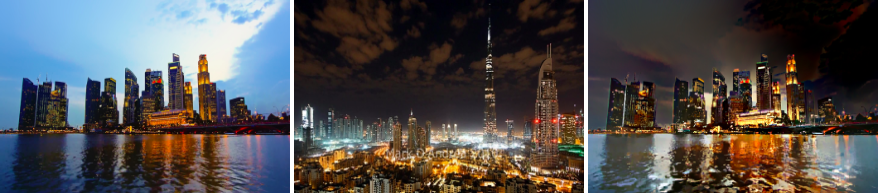
\includegraphics[width=.85\textwidth]{dps_o_1}
    \caption{Deep Photo Style Transfer官方实验样例图}
    \label{fig:dps}
\end{figure}

% wc ~ 1000

\subsubsection{Fast Photo Style}[Fast Photo Style]

\textbf{Fast Photo Style.}\cite{fps}\quad  提到其他的风格转换技术中存在的问题:合成的图片往往会有不一致的风格特征,且有比较明显不真实部分。这也是该算法主要希望解决的问题。此外,算法也希望最后合成的图片应该跟用相机拍摄的照片一样真实,相较其他的主要基于色调匹配来风格化图片的技术,不同的是Fast Photo Style还关注输入图像中个内容特征的学习与提取。

\begin{figure}[t]
    \centering
    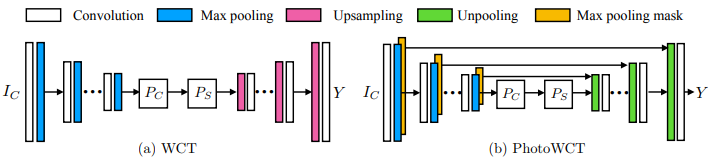
\includegraphics[width=.8\textwidth]{wct}
    \caption{}
    \label{wctf}
\end{figure}

该算法的风格化主要由两个关键步骤组成。第一步是名为PhotoWCT的样式转换$F_1$。给定一个样式图片$I_S$,$F_1$将$I_S$的风格迁移到内容图片$I_C$上,同时最小化最后的输出图片中的结构变化。虽然$F_1$可以很好的样式化$I_C$,但在语义上比较相近的区域上经常会合成样式不一致的图片。因此该算法使用了一个光滑函数$F_2$,试图借此来消除这些“坏掉的”部分。算法整体可以表达成下面的两步映射函数:
\begin{align}
    F_2(F_1(I_C,I_S),I_C)
\end{align}

PhotoWCT是基于WCT\cite{wctp}算法,为了实现真实的图片样式合成,它使用了一个新奇的网络架构。为了使用WCT,对于一般的图片重建的自动编码器被首先训练。一般的训练过程使用的是VGG-19模型作为编码器\varepsilon,并且训练解码器$D$来重建输入图片。解码器和编码器行程对称,在行为上互为逆反操作。当自动编码器训练好了,一堆映射函数就被插入到网络中,通过白化($P_C$)和彩色花($P_S$)变换来行使样式化操作。主要思想是通过两个映射函数直接将内容图像的特征相关映射到样式图片中。具体地,给定一堆内容图片$I_C$和样式图片$I_S$,首先提取除向量化的VGG特征$H_C=\varepsilon(I_C)$和$H_S=\varepsilon(I_S)$,然后再通过下面公司来转换内容特征$H_C$:
\begin{align}
    H_{CS}=P_SP_CH_C
\end{align}
这里$P_C=E_C\Lambda_C^{-\frac{1}{2}}E_C^T$,$P_S=E_S\Lambda_S^{\frac{1}{2}}E_S^T$,其中$\Lambda_C$和$\Lambda_S$是堆成三角矩阵,且有相同的协方差矩阵$H_CH_C^T$和$H_SH_S^T$。矩阵$E_C$和$E_S$是各自对用的特征向量的正交矩阵。转换后,特征方差会匹配样例图片的特征空间,即$H_{CS}H_{CS}^T=H_SH_S^T$。最后样例图片可以通过直接将转换后的特征映射到解码器$Y=D(H_{CS})$来合成。

为了解决合成图片部分区域扭曲不真实的问题,算法将原本的采样层替换成了池化层,PhotoWCT函数可以表示成:
\begin{align}
    Y=F_1(I_C,I_S)=\overline{D}(P_SP_CH_C)
\end{align}
这里的$\overline{D}$是解码器,包含了池化层的信息,用作后面的图片重构。图片\ref{wctf}展示了PhotoWCT和WCT之间的网络结构差异。

\begin{figure}[t]
    \centering
    \subfigure[]{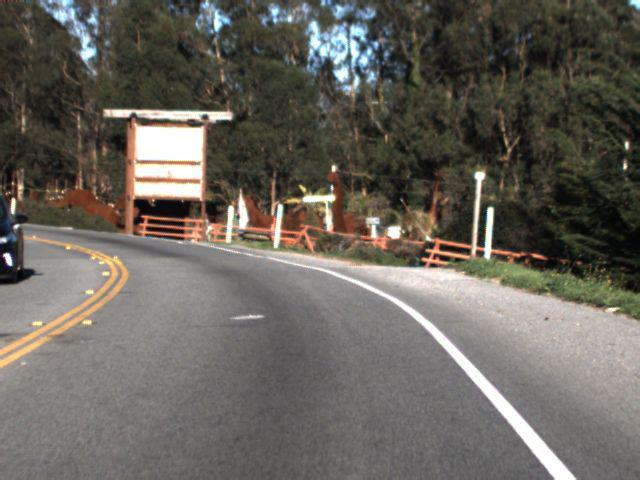
\includegraphics[width=.23\textwidth]{fps/origin}}
    \subfigure[]{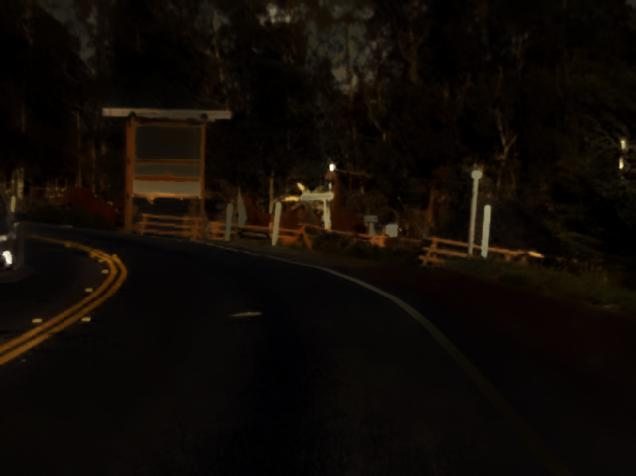
\includegraphics[width=.23\textwidth]{fps/night}}
    \subfigure[]{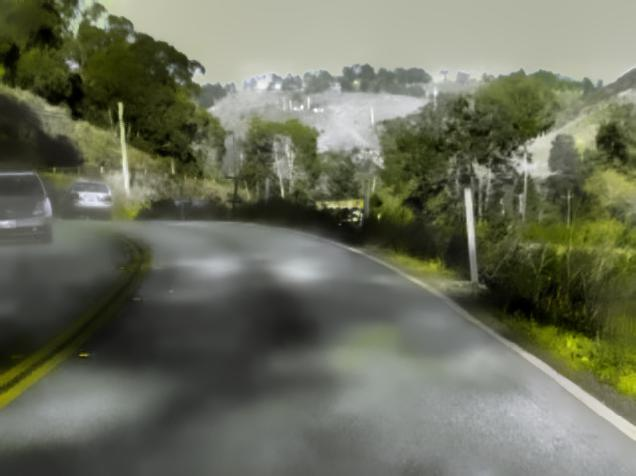
\includegraphics[width=.23\textwidth]{fps/rain}}
    \subfigure[]{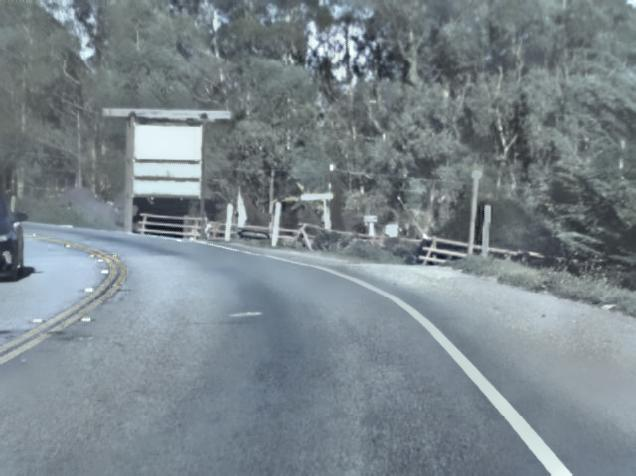
\includegraphics[width=.23\textwidth]{fps/snow}}
    \subfigure[官方实验样例图]{
        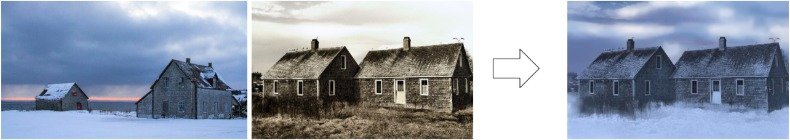
\includegraphics[width=.85\textwidth]{fps_o_1}
    }
    \caption{Fast Photo Style实验结果样例图}
    \label{fps-result}
\end{figure}

实际实现中,该算法官方给出了一个提前训练好的模型,其编码器$\varepsilon$使用了VGG-19网络结构中的conv1-1到conv4-1层,其权值由用ImageNet提前训练好的权值给定。训练数据集使用了微软COCO数据集\cite{coco}。总体来说,Fast Photo Style是一个能够实现快速合成真实图片风格转换的技术,它主要由格式化步骤和真实光滑化(photorealistic smoothing)步骤组成。该算法对上述两个步骤都给出了有效地闭环解决方案。

我们使用该模型进行了雨天、网上和雪天场景的转换,图\ref{fps-result}展示了最终实验结果样例图以及Fast Photo Style官方图像风格转换实验样例图。

% wc ~ 1000
% fast photo style要求content和style image内容尽可能相近

\subsubsection{Fast Neural Transfer}

\textbf{Fast Neural Transfer.}\cite{FNT} 该算法计算单个像素的损失函数时不止考虑低层级的像素信息,还利用损失网络中的高层级特征表示的感知损失函数来训练算法的网络结构。训练过程中,感知损失能够比单个像素损失函数更好的测量出图像之间的相似度。除了图像风格的转换,Fast Neural Transfer还可用于图像的分辨率升级等应用。它通过利用感知损失函数训练的前向转换神经网络将前向图像转换任务和优化后的图像合成技术结合了起来。

\begin{figure}[!bh]
    \centering
    \subfigure[]{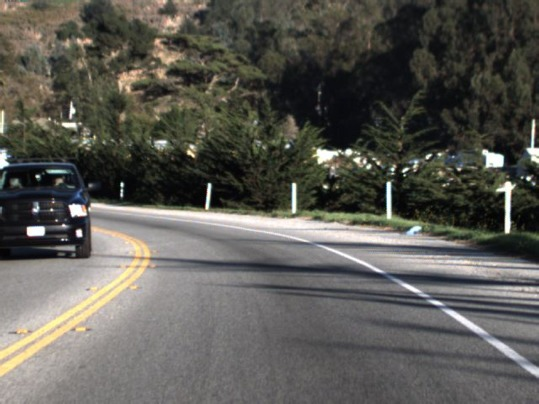
\includegraphics[width=.23\textwidth]{FNT/origin}}
    \subfigure[]{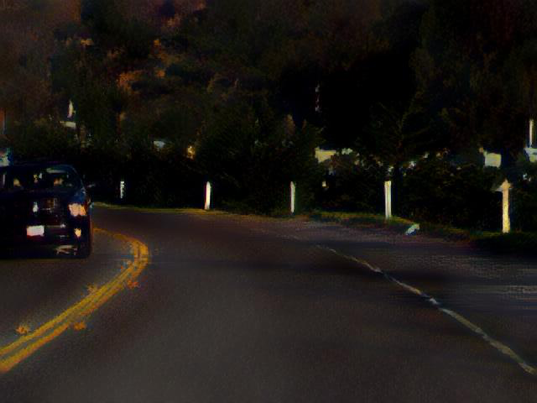
\includegraphics[width=.23\textwidth]{FNT/night}}
    \subfigure[]{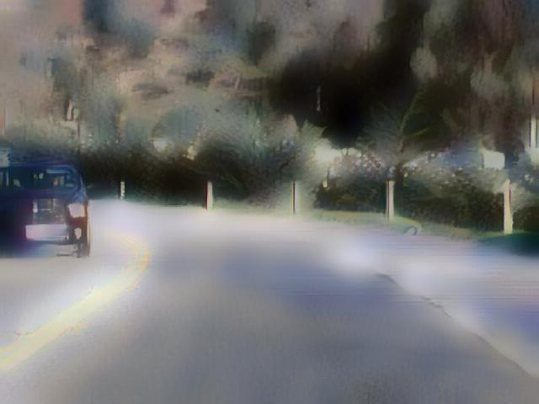
\includegraphics[width=.23\textwidth]{FNT/fog}}
    \subfigure[]{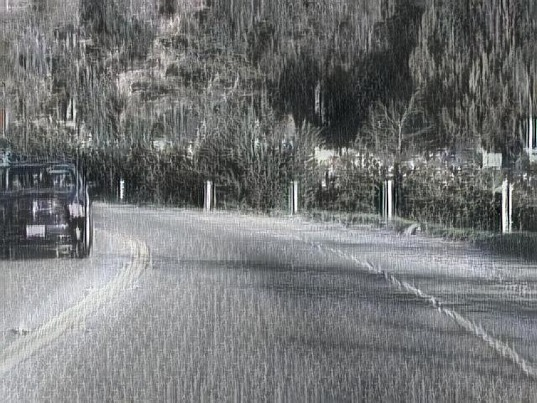
\includegraphics[width=.23\textwidth]{FNT/snow}}
    \subfigure[官方实验样例图]{
        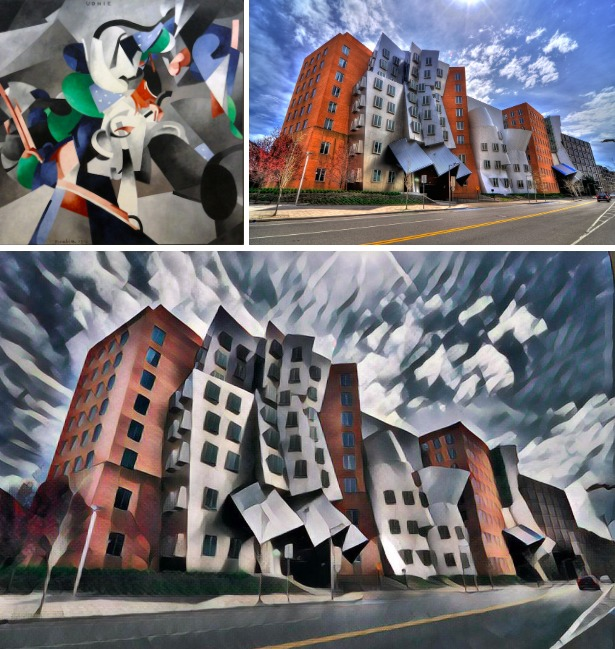
\includegraphics[width=.75\textwidth]{fnt_o_1}
    }
    \caption{Fast Neural Transfer实验结果样例图}
    \label{fnt-result}
\end{figure}

该算法系统由两部分:图像转换网络$f_w$和损失网络$\Theta$。其中损失网络用来定义多个损失函数$\ell_1,\dots,\ell_k$。图像转换网络是一个由权值$W$参数化的深度残差卷积神经网络。它通过映射函数$\hat{y}=f_W(x)$将输入图片$x$转换成输出图片$\hat{y}$。每个损失函数都会计算一个标量值$\ell_i(\hat{y},y_i)$来测量输出图片$\hat{y}$和目标图片$y_i$之间的距离。该图像转换网络的训练使用了一个复杂的梯度下降算法来最小化损失函数的权值组合:
\begin{align}
    W^*=\arg \min_W E_{x,\{y_i\}}\Big[\sum_{i=1}\lambda_i\ell_i(f_W(x),y_i)\Big]
\end{align}

为了解决单个像素损失的缺点,且是损失函数更好的测量出不同图像间的语义距离,该算法使用了提前为图像分类训练好的模型。因为这些模型一般都是卷积神经网络,且都在训练阶段学习了将我们想在损失函数中测量的语义信息编码的能力。因此,算法中为了定义损失函数,选择利用提前为图像分类训练好的网络模型$\Theta$作为固定的损失网络。

对于样式转换器,其输入和输出都是像素形状为$3\times 256 \times 256$的彩色图片。对于采样因子为$f$的高清图片,其输出是像素形状为$3\times288\times288$,输入为$3\times288/f\times288/f$。因为图像转换网络是全卷积的,所以在测试阶段它们可以用于任意分辨率的图片上。

算法中提出特征重建损失值是不同特征空间中的欧几里得距离:
\begin{align}
    \ell_{feat}^{\Theta,j}(\hat{y},y)=\frac{1}{C_jH_jW_j}||\Theta_j(\hat{y})-\Theta_j(y)||_2^2
\end{align}
当输出图片与目标图片的内容差异时特征重建损失函数会惩罚输出图片,对于输入$x$,网络$\Theta$中第$j$层的激活函数记为$\Theta_j(x)$,该函数是形状为$C_j\times H_j\times W_j$的特征图谱,定义Gram矩阵为$C_j\times C_j$的方阵,其元素有下面的公式给定
\begin{align}
    G_j^{\Theta}(x)_{c,\hat{c}}=\frac{1}{C_jH_jW_j}\sum_{h=1}^{H_j}\sum_{w=1}^{W_j}\Theta_j(x)_{h,w,c}\Theta_j(x)_{h,w,\hat{c}}
\end{align}

除此之外,该算法还定义了一个简单的损失函数:像素损失函数是输出图片$\hat{y}$和目标图片$y$间的欧氏距离。如果两者的尺寸形状都为$C\times H\times W$则像素损失为$\ell_{pixel}(\hat(y),y)=||\hat{y}-y||_2^2/CHW$。图\ref{fnt-result}为该算法在我们的数据集上实验的结果样例图以及Fast Neural Transfer官方的实验结果样例图。 

\subsubsection{UDPIR} 

\newmodel{UDPIR} 该算法的主要改进点在于它提出图像逆反表示的一种方法,该方法只利用图像表征的信息,以随机噪声图片为初始值,从而可以只包含表征自身的数据信息。图像的逆反表征问题本质上是寻找一张表征与给定图像最为接近和匹配的图片,即给定表征函数$\Phi:\mathbb{R}^{H\times W\times C}\to \mathbb{R}^d$和逆反表征$\Phi_=\Phi(x_0)$,图像可通过最小化下面的目标函数实现重建:
\begin{align}
    x^*=\min_x\in \mathbb{R}^{H\times W\times C}\mathb{l}(\Phi(x),\Phi_0)+\lambda\mathb{R}(x)
\end{align}
此处的$\mathb{l}$表示重建图像的表征与给定图像表征之间的距离,文献中具体的函数使用里欧几里得距离函数:
\begin{align}
    \mathb{l}(\Phi(x),\Phi_0)=||\Phi(x)-\Phi_0||^2
\end{align}
算法的具体实现中,依然采用了提前训练好的VGG19卷积神经网络的结构来重建图像,由于文献中没有给出官方的实验代码,我们依照文献中的方法复现了MNIST数据集中数字图像的重建,但是后面试图对路况图像进行重建实验中我们发现,该算法对于数据集中$256\times 256$图片的重建合成耗时过长,约2小时一张,效率过低,因此我们放弃了对该模型的进一步实验。

\subsubsection{Targeted Style Transfer}

\newmodel{Targeted-Style-Transfer} 该算法不同之处在于只修改目标图像的某一部分而不是全部,比如只修改图片中的某一个物体而不改变物体的背景和周围场景。算法实现中除了使用了基于深度神经网络的图片修改技术还需要图像语义分割技术的协助,在物体边界的光滑化和去锯齿化中使用了马尔可夫随机场模型。

算法的具体实现是基于Gatys提出的图像风格转换技术\cite{nst},给定包含了指定风格的原图片$s$,和目标转换图片$t$,算法目标是将图像$x$转换到风格与$t$类似的新图像中,但是其中的纹理信息保留。以上可以用下面的最小方差函数表示:
\begin{align}
    \min_x ||F(x)-F(t)||^2+||C(x)-C(s)||^2
\end{align}
$F(\cdot)$是将图像映射到对应的深度特征空间的映射函数,$C(\cdot)$是将图像映射到对应特征空间协方差的映射函数。

下图\ref{fig:tst}是Targeted Style Transfer的实验样例图,在实现我们的路况图像风格转换实验中,由于我们的需求往往是对道路或者天气的像素风格转换,而且转换后㛑需要对整个图像的整体风格也要做相应的调整,从而使得合成图像尽可能的真实。这使得我们需要对原始图片做大量的语义分割工作,而目前还没有专门这对这类工作的自动化流程代码出现,这使得我们要对整个路况图像库坐语义分割的预处理变得成本巨大,导致难以实现,因此我们也放弃了对该模型的进一步实验。 

\begin{figure}[h]
    \centering
    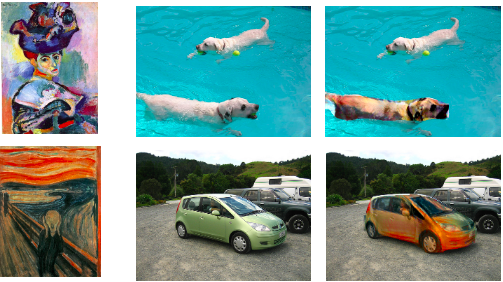
\includegraphics[width=.8\textwidth]{results/tst}
    \caption{Targeted Style Transfer实验样例图片}
    \label{fig:tst}
\end{figure}

\subsubsection{Feedforward style transfer}

\newmodel{Feedforward-style-transfer} 该算法对于图像转换任务使用了前向转换网络,与其他算法不同的是,其损失函数不是依靠图像中的低级信息,即每个像素之间的距离,而是使用图像中的高级特征之间的距离,即感知器损失函数。模型训练过程中,感知器损失函数对图像之间的差异度量比像素见的损失函数更加可信。

该模型的主要优点是在与其他图像风格转换算法取得相似效果的同时,其模型的训练更高效。其模型训练中使用的损失函数也是创新点所在,具体训练过程使用了stochastic梯度下降算法,其损失函数为:
\begin{align}
    W^*=\min_W\mathb{E}_{x,\{y_i\}}[\sum_{i=1}\lambda_il_i(f_W(x),y_i)]
\end{align}

由于该算法跟其他的图像转换技术算法一样,主要用于艺术画的图像合成,其实验结果样例图\ref{fig:fst}如下,所以我们将该算法用在路况图像转换上,最后的合成的路况图片也都太过艺术画了,与真实场景的驾驶路况场景差距太大,因此我们放弃了该模型的进一步实验数据统计和总结。 

\begin{figure}[h]
    \centering
    \includegraphics[width=.8\textwidth]{results/fst}
    \caption{Feedforward style transfer实验结果样例图}
    \label{fig:fst}
\end{figure}

% wc ~ 800

\subsubsection{Texture Nets}

\textbf{Texture Nets.}\cite{texture-nets}\quad 使用了前向生成网络来实现图像合成和风格化功能。该算法主要针对图像的纹理风格转换,文献\cite{texture-nets}中指出图片的纹理数据分布可由样本纹理数据$x_0$推导出,比如$x\sim p(x|x_0)$。在风格迁移中,分布是由图像$x_0$的视觉样式表征和另一张图片$x_1$的视觉内容表征推导出。特别的,为了从样本图片$x_0$合成纹理,这个问题可以表示为:
\begin{align}
    \min_{x\in \chi}||\Phi(x)-\Phi(x_0)||_x^2
\end{align}
对图像纹理来说,一般会假设$p(x)$是一个静态马尔科夫随机链。纹理$x_0$可以通以下公式估算局部区域的平均统计特征值:
\begin{align}
    \phi(x_0)=\frac{1}{|\Omega|}\sum_{i=1}^{|\Omega|}\psi_oF(x_0;i)\approx E_{x\sim p(x)}[\phi_oF_l(x;0)]
\end{align}

\begin{figure}[b]
    \centering
    \subfigure[]{\includegraphics[width=.45\textwidth]{texture-nets/1}}
    \subfigure[]{\includegraphics[width=.45\textwidth]{texture-nets/2}}
    \subfigure[官方实验样例图]{
        \includegraphics[width=.7\textwidth]{tn_o_1}
    }
    \caption{Texture Nets实验结果样例图} 
    \label{tn-example}
\end{figure}

同其他的图像风格转换技术类似,该算法的损失函数也是从文献\cite{nst}中推导出来的,图像的统计数据通过固定的提前训练好的卷积神经网络(通常是VGG网络)提取出来。其Gram矩阵可以定义成一个向量矩阵和特征图谱的点积:
\begin{align}
    G_{ij}^l(x)=<F_I^l(x),F_j^l(x)>
\end{align}
因为网络属性是卷积的,所以每个点积都是所有空间特征$i$和$j$激活函数的乘积之和。模型在实际训练过程中,将Gram矩阵$G^l,l\in L_T$组合用作纹理描述表征体,这里的$L_T$包含了表征体卷积网络中卷积层的下标指数。以上可以推导除下面的图像$x$和$x_0$之间的纹理损失:
\begin{align}
    L_T(x;x_0)=\sum_{l\in L_Y}||G^l(x)-G^l(x_0)||_2^2
\end{align}
除了纹理损失函数,该算法还提出基于卷基层$l\in L_C$的输出$F_i^l(x)$来比较图片差异:
\begin{align}
    L_C(x;y)=\sum_{l\in L_C}\sum_{i=1}^{N_t}||F_i^l(x)-F_i^l(y)||_2^2
\end{align}
这里的$N_t$是第$l$层的特征通道个数。与纹理损失的主要差别在于内容损失在对应的空间区域比较特征激活函数,因此保留了空间位置信息。因此内容损失函数对于内容信息保留来说更合适,但对于纹理信息去并不合适。

算法中具体的学习过程是通过调整生成器$g(y_i,z_i;\theta)$参数$\theta$来最小化内容和纹理损失函数的组合值:
\begin{align}
    \theta_{x_o}=\min_{\theta}E_{z\sim Z;y\sim Y}[L_T(g(y,z;\theta),x_0)+\alpha L_C(g(y,z;\theta),y)]
\end{align}
这里的$Z$表示纹理合成图片的噪声分布,$y$是真实图片的实际分布,$\alpha$是平衡纹理/样式和内容的参数。图\ref{tn-example}为该模型的最终实验结果样例图以及Texture Nets官方实验结果样例图。


\section{本章小结}

本章主要介绍了该实证研究项目的实验方法设计:即实验数据比较指标的设计,实验比较模型的筛选历程,以及对选取的每个模型进行了简要的原理介绍。在模型筛选过程中本实验初期进行了大量的实验,由前文介绍的,最终由于种种原因:源码未开放,无法针对每个技术模型收集到最匹配的训练数据集,合成图与我们路况天气风格转换与合成的需求有较大出入等原因进行了大量的取舍,最终记录在论文中的是我们重点实验过的模型,参与实验最后数据的统计与比较的一共有8个DNN模型,主要为对抗生成网络和图像风格转换迁移技术。

此外所有的实验都是在Ubuntu 16.04 LTS操作系统,8核GeForce GPU的计算机上进行的,所有的合成图像数据统一使用Python pickle包压缩后存储于MySQL数据库中,未来计划开源在GitHub上。

% wc ~ 800


\chapter{基于深度学习的自动驾驶系统蜕变测试框架}

\section{引言}

上一章中提到了DeepTest设计了一个试图模拟现实世界驾驶场景的图像,进而自动生成测试用例的测试系统,但它合成图像的主要方式是在原驾驶图像上应用仿射变换,添加各种效果图层,比如雾天、雨天和模糊效果
,然后检测自动驾驶系统在原图和合成图上的输出行为是否一致。通过大量的原始和合成后的驾驶场景图,DeepTest以一种相对快速和廉价的方式成功地在一些开源的自动驾驶模型中检测出了各种不一致的驾驶行为。

\begin{figure}[h]
    \centering
    \subfigure[DeepTest]{
        \includegraphics[width = 0.7\textwidth]{deeptest_effect}
    }
    \subfigure[蜕变测试框架]{
        \includegraphics[width = 0.7\textwidth]{deeproad_effect}
    }
    \caption{天气场景合成效果图比较}
    \label{label-deep}
\end{figure}

但是我们认为DeepTest用于合成测试用例的方法并不能真实地反应出现实中的驾驶场景。比如现实中由车载摄像头拍摄的驾驶场景很少会有仿射变换后的效果,通过应用在原图上的雾天、雨天和模糊效果来简单地模拟对应的天气场景下的图像也显得很不真实,这也降低了DeepTest检测结果的有效性和可靠性。比如
下图\ref{label-deep}a左图为DeepTest中添加的雾天效果,可以明显看出图中很多部分呈现出扭曲的状态,感觉就像是简单地调暗原图像素,然后加上简单的烟雾效果,事实上,我们简单地利用PhotoShop中的像素调节和图像叠加功能也合成了DeepTest中的图像。下图\ref{label-deep}a右图则显示了DeepTest使用的雨天效果变换,类似地,DeepTest也是通过简单地将许多白色线条加到了原图上来模拟雨天场景的。这样合成的雨天场景图片相比前者更加的不真实,因为在现实的雨天场景中,摄像头上往往会有雨滴,从而呈现出模糊的效果。DeepTest中只有极少的合成图像跟真实的驾驶场景类似,使得我们很难判断利用DeepTest检测出的错误驾驶行为到底是由原本基于深度神经网络的自动驾驶系统的缺陷导致,还是由于DeepTest本身的测试技术的不足导致的。除此之外,还有许多各种可能的真实驾驶场景是不能通过简单的图像变换技术来合成模拟的。比如大学天气下的道路场景,对于道路和合成渲染过程需要多种复杂的变换同时应用到原图上,道路旁边的物体,比如树木也是如此。

为了沿用DeepTest测试的核心思想,自动地为自动驾驶系统合成大量的真实驾驶场景的图像,我们参考DeepRoad测试技术设计了一个无监督测试框架。利用深度学习中的对抗生成网络技术来合成一些很难由人工采集到的各种天气场景下的路况图像。除此之外,我们基于DeepTest的工作,设计了一套针对基于深度神经网络自动驾驶系统的一个蜕变测试模块,核心思想为:无论真实的驾驶场景图像对于各种天气场景被以何种方式合成,自动驾驶系统对于原图和合成图做出的驾驶行为输出我们期望始终保持一致。基于此点,蜕变测试框架使我们能够测试基于深度神经网络的自动驾驶系统在各种天气场景下的精确性和可靠性,合成的各种极端天气场景下的图像集,比如大雪大雨天气的场景图像也能够扩充自动驾驶系统原有的数据集测试用例覆盖率,从而有助于提高自动驾驶系统的稳定性和鲁棒性。图\ref{label-deep}b为蜕变测试框架合成的雪天和雨天的驾驶场景图像,已经很难从真实的图像中区分,并且通过简单的图像转换技术很难合成类似的效果。

虽然蜕变测试框架可以用来合成各种天气场景的驾驶图像,在我们实验过程中,我们主要针对雪天和雨天场景进行了驾驶场景图像的合成工作。基于对抗生成网络技术,我们利用网络爬虫技术Scrapy从Youtube视频网站上收集了2组极端天气场景下的驾驶图像集,将真实的驾驶场景图像转换到对应的天气场景下的驾驶场景。此外,我们将合成的图像用于测试Udacity开源的自动驾驶系统\cite{udacity_as},实验结果显示蜕变测试框架检测出了上千种这些系统不同级别的行为不一致现象,表明自动驾驶系统的测试工作还有很大的提升空间。

\section{方法}

\subsection{深度神经网络蜕变测试}

蜕变测试在传统软件测试方法里被广泛应用于测试用例的自动生成以及BUG检测,蜕变测试的强大之处主要在于它能通过各种蜕变关系解决传统测试的Oracle问题。令$p$为程序的数学表示形式:一个将程序输入映射到程序输出的函数,即$p(i) = o$,同样地,令函数$f_I$和$f_O$分别表示程序输出集合输出集的映射函数,则一个蜕变关系可表示为:
\begin{gather}
    \centering
    \forall i, p(f_I(i))=f_O(p(i))
    \label{f:mt}
\end{gather}
基于这样的蜕变关系,令$\hat{p}$表示程序$p$的一个具体实现,则我们可以通过检测公式$\hat{p}(f_I(i))=f_O(\hat{p}(i))$是否对任意输入$i$都成立来测试程序$\hat{p}$的鲁棒性。通过利用蜕变关系交叉检验程序输入输出,从而测试程序具体实现的方法称为蜕变测试。例如给定一个实现$sin$函数的程序,我们可以利用蜕变测试来构造各类新的测试用例,而不用担心测试的对照物,即测试Oracle问题。对任意用于测试$sin$函数的输入$i$,有许多客观事实可以用于该测试的蜕变关系,比如$sin(-i)=sin(i)$以及$sin(i+2\pi)=sin(i)$。特别的对于这里蜕变关系的第一个例子有:$f_I(i)=-f_O(i)=-i$,对于第二个例子则是$f_I(i)=f_O(i)=i$。利用这样的蜕变关系,我们能够将已有的测试用例通过$f_I$生成一些新的测试用例,然后基于$f_O$来检验程序的输出。

在本工作中,我们进一步地将蜕变测试应用到了基于深度神经网络自动驾驶系统的测试当中。正式地,令$DNN$表示将每张路况图像映射到预测的方向盘拐角信号的基于深度神经网络的自动驾驶系统,给定原始图像集$\mathbb{I}$,定义各种图像变换$\mathbb{T}$,变换可以改变图像的路况场景,而不影响每张图像$i\in \mathbb{I}$的预测结果(即预测的拐角对于雨天和雪天场景下相同的路况图片应该几乎一致)。通过这样的方式,对于利用各类额外的变换图像输入来测试自动驾驶系统,我们可以得到下面的蜕变测试:
\begin{gather}
    \forall i \in \mathbb{I} \wedge \tau \in \mathbb{T}. DNN[\tau(i)]=DNN(i)
\end{gather}

\subsection{基于深度神经网络的路况图像变换}

关于自动驾驶系统测试的最新工作DeepTest\cite{DeepTest}也将蜕变测试用在了基于深度神经网络的自动驾驶系统测试中,但它只作了一些简单的图像合成转换,例如添加雾天、雨天和雪天的图层,因此导致有以下问题的存在:1). DeepTest可能会产生不真实的测试用例;2). DeepTest不能模拟复杂的道路场景变换(比如雪天场景)。

为了完善DeepTest工作,全自动地产生各种真实场景下的路况图像,我们利用UNIT\cite{UNIT},一个基于深度神经网络的方法来进行无监督图像到图像的变换。UNIT的核心思想是不同图像集的一组图像可以被映射到一个共享潜在空间,并有相同潜在表征。通过这样映射的方式,可以将来自某个图像集的图像(比如原始的路况图像),UNIT可以自动地合成另对应于另一个图像集(比如雨天的路况图像集)的图像,具体实现上,UNIT由对抗生成网络变分自编码器构成。

\begin{figure}[h]
    \centering
    \includegraphics[width=.7\textwidth]{UNIT}
    \caption{UNIT模型结构}
    \label{unit-struct}
\end{figure}

图\ref{unit-struct}描述了UNIT模型的基本架构,其中$S_1$和$S_2$记为两组不同的图像集,$E_1$和$E_2$为2个将图像集分别从$S_1$和$S_2$投射到共享隐空间$Z$的自编码器。令$x_1$和$x_2$为共享同内容信息的对应图像,理想情况下$E_1$和$E_2$能将他们编码到相同的隐向量$z$。$G_1$和$G_2$为2个不同图像域的生成器,可将隐向量分别映射回$S_1$和$S_2$图像集中。$D_1$和$D_2$是两个判别器,可以检测出图像属于$S_1$还是$S_2$。理想情况下,判别器不能区分输入图像是来自目标图像域还是训练好的生成器。基于上述的自编码器和生成器,UNIT可以用来在两个不同图像域中转换图像,比如图像$x_1$可以通过$G_2(E_1(x_1))$转换到图像集$S_2$中。

UNIT的学习目标可以分解为优化以下3个损失函数:
\begin{itemize}
    \item \textbf{变分自编码器损失函数} 对每组编码器和生成器$<E_i,G_i>$最小化图像的重构损失。
    \item \textbf{对抗生成网络损失函数} 在对抗器和判别器对$<G_i,D_i>$的最小最大函数中找到最优值,使得$D_i$不能区分图像$x_i$是来自原图像集$S_i$还是生成器$G_i$。
    \item \textbf{循环一致损失函数} 对每组$<E_i,G_j,E_j,G_i>$最小化他们的循环重构损失,理想情况下有$x_1=G_1(E_2(G_2(E_1(x_1))))$以及$x_2=G_2(E_1(G_1(E_2(x_2))))$
\end{itemize}

总的损失函数可归纳为以下:
\begin{equation}
\begin{aligned}
    \min_{E_1,E_2,G_1,G_2}\max_{D_1,D_2}\mathb{L}_{CC_1}(E_1,G_2,E_2,G_1)+ \\ 
    \mathb{L}_{CC_2}(E_2,G_1,E_1,G_2) + \mathb{L}_{VAE_1}(E_1,G_1)+\mathb{L}_{VAE_2}(E_2,G_2)+ \\
    \mathb{L}_{GAN_1}(D_1,G_1) + \mathb{L}_{GAN_2}(D_2,G_2)
    \label{f:unit}
\end{aligned}
\end{equation}

\subsection{测试框架整体架构}

\begin{figure}[h]
    \centering
    \includegraphics[width=.7\textwidth]{deeproad_wf}
    \caption{蜕变测试框架架构}
    \label{dp-wf}
\end{figure}

上图\ref{dp-wf}为我们为基于深度神经网络自动驾驶系统设计的蜕变测试框架。如图所示,我们的蜕变测试框架首先从目标图像集(即一组晴天路况图像集和一组雨天路跨那个图像集)选出一组无配对的训练图集,然后利用无监督框架UNIT将这两组图像集利用公式\ref{f:unit}中的损失函数,映射到同样的隐空间。我们从Udacity开源的真实路况数据集\cite{udacity_dataset}采样了晴天路况图,从Youtube视频收集了雪天和雨天的路况图集,然后将他们作为UNIT的训练集进行模型的训练。模型训练完成后,再利用成型的UNIT将整个Udacity图像集转换成另一个场景的路况图像集(雪天场景或者雨天场景)。即给定任一原始的晴天驾驶场景图像$i$,测试框架可以利用训练好的UNIT模型合成出原始图像在另一个天气场景下对应的图像(即雨天场景),记为$\tau(i)$。最后测试框架将每组配对的真实图像和合成图像送入自动驾驶系统进行测试,即检测$DNN[\tau(i)]=DNN[i]$是否成立,从而检测自动驾驶系统的不一致输出行为。因为路况合成图像对驾驶行为,即方向盘拐角,不会有较大影响,因而任一不一致的输出都可能反应了自动驾驶系统在测试框架下显示出的鲁棒性问题。

\section{实验}

\subsection{实验数据和数据预处理}

我们使用由Udacity提供的真实数据集作为检验自动驾驶系统不一致行为的基准数据,从该数据集中选取了2段高速公路驾驶视频,视频中道路的光线和路况随着时间变化有明显的改变。为了训练相应的UNIT模型,我们也从Youtube上收集了各种极端场景下的路况图像。具体实验阶段,我们选择了雪天和大雨天气下的路况图像来转化真实场景的驾驶路况图像。为了扩充收集到图像集的多样性,我们只搜索了时长超过20分钟的视频。在大雨场景的视频里,通常会有雨刷扫过车窗的情形,这对图像数据而言是噪声数据,因此在数据的预处理阶段,我们人工的检查和筛除了有雨刷出现的图像。除此之外,实验中所有使用的图像在实验之前都被裁剪成$240\times 320$的大小,并且对从Youtube上收集的视频进行了低频采样,以避免有过于相近的连续图像帧出现在最终的数据集里。

\subsection{自动驾驶系统模型}

我们基于Udacity开源的3个深度神经网络自动驾驶系统模型对我们的测试框架进行评估,分别有:Autumn\cite{autumn},Chauffeur\cite{Chauffeur}和Rwightman\cite{Rwightman}。我们使用这3个模型作是因为他们都是预训练好的模型,且可以直接在合成数据集上进行驾驶拐角预测。其中Rwightman模型的实现细节没有公开,但是基于黑盒测试原理,我们的方法目的是检测模型输出的不一致行为而不是定位软件的错误,因此我们仍然使用Rwightman作为我们的评价模型。

\textbf{Autumn}. Autumn由一个数据预处理模块和一个卷积神经网络构成。具体实现上,Autumn首先计算输入图像的光线流,然后将他们输入到卷积神经网络中预测方向盘拐角。Autumn的网络结构为:3层步长为2的$5\times 5$的卷积层,2层$3\times 3$的卷积层加上5个全连接层。模型由OpenCV,Tensorflow和Keras框架实现。
\textbf{Chauffeur}. Chauffeur由一个卷积神经网络和一个有LSTM单元递归神经网络(RNN)构成。工作流程为:卷积神经网络首先提取输入图像的特征,然后利用RNN对之前的100张连续图像进行方向盘拐角预测。该模型也是通过Tensorflow和Keras实现的。

\subsection{评价指标}

基于我们的假设,如果方向盘拐角的预测值在修改了路况图像的天气场景后不发生改变的话则被测试的自动驾驶系统可被视为是稳定的。但是这个假设条件太苛刻了,因为由于图像场景改变导致的微小的拐角差也可以落在安全的拐角区域。因此,我们放宽了之前的假设条件,如果原图和合成图的预测拐角差值能够在一定的误差范围内,我们也接受该预测拐角值。我们将被测试的自动驾驶系统中出现的不一致预测行为次数定义为:
\begin{gather}
    IB(DNN,\mathbb{I})=\sum_{i\in \mathbb{I}}f(|DNN[i]-DNN[\tau(i)]|>\epsilon)
\end{gather}
这里的$DNN$记为自动驾驶系统模型,$\mathbb{I}$为真实场景的驾驶图像数据集,$i$为图像集$\mathbb{I}$中第$i$张图像。$\tau$记为能够实现输入图像天气场景转换的图像生成器。函数$f$为输出为1或0的指示函数,$\epsilon$为允许的误差范围。

\subsection{实验结果}

\begin{figure}[htb]
    \centering
    \includegraphics[width=\textwidth]{inconsist}
    \caption{自动驾驶系统在真实图和合成图上表现的不一致行为}
    \label{inconsist}
\end{figure}

图\ref{inconsist}为检测到自动驾驶系统不一致行为的样例图,第一行为雪天场景的图,第二行为雨天场景的图。每张小图中,蓝色的字为模型的名称,红色和绿色的字为真实图和合成图的预测拐角值。图中的曲线描述了预测值即方向盘拐角,帮助我们检验差值。从图中我们可以观察到模型Autumn模型中出现的不一致行为数最多,反之,模型Rwightman相对而言是最稳定的自动驾驶系统模型。图\ref{inconsist}也表明测试框架能够在不同天气场景下对真实的自动驾驶系统发现各种不一致行为。比如像Autumn和Chauffer的自动驾驶系统模型(在Udacity的自动驾驶系统竞赛中它们是排名最高的2个算法),在晴天的驾驶场景下表现相当出色,但在雨天或雪天的场景下可能会撞向路边或是其他的车辆。

\begin{figure}[]
    \centering
    \includegraphics[width=.5\textwidth]{inconsist-t}
    \caption{不同天气场景及误差限下检测到的不一致行为数}
    \label{inconsist-t}
\end{figure}

图\ref{inconsist-t}展示了在不同天气场景、不同的误差界限下对各个自动驾驶系统模型检测到的不一致行为的具体数量。比如当检测的场景为雨天,误差限设为$10\degree$时,测试框架对3中自动驾驶系统分别检测到了5279,710和656种不一致行为。从表中我们也观察到Autumn在两种天气场景下检测到的不一致行为数目是最多的。我们认为一个可能的原因是因为Autumn是完全基于基于卷积神经网络的结构,不能像反馈神经网络一样利用到前验历史信息,因而导致系统不能在所有的驾驶场景下都能表现出很好的鲁棒性。另一方面,Rwightman比其他两个模型在雨天和雪天场景,以及各个误差限下都表现出更好的驾驶行为一致性。以上表明测试框架不仅能检测出自动驾驶系统上千种不一致的驾驶行为,还能就每个自动驾驶系统的鲁邦性作出评估,比如仅靠Udacity原始的数据集,很难发现类似Autumn这样的自动驾驶系统在雨天和雪天场景下的局限性。

\section{本章小结}

我们设计了一个基于DeepRoad\cite{DeepRoad},利用无监督对抗生成网络的技术来测试深度神经网络自动驾驶系统的蜕变测试框架。它使用蜕变测试技术检测自动驾驶系统在不同的天气场景下所表现出不一致的驾驶行为。除此外,实验结果表明该测试框架在检测自动驾驶系统鲁邦性上也有很好的应用价值。目前它只支持两种天气场景下的测试用例转换,在后面的章节将介绍我们针对提高自动生成的测试用例质量,即驾驶场景图像的合成质量,以及驾驶场景的种类扩充所做的后续工作。
\chapter{基于对抗生成网络的自动驾驶系统测试实证研究}

\section{引言}

上一章讲到的DeepRoad测试框架在自动驾驶系统鲁棒性和稳定性测试上取得了成功,对Udacity开源的Autumn\cite{autumn},Chauffeur\cite{Chauffeur}和Rwightman\cite{Rwightman}3个自动驾驶系统都检测出了不同程度的驾驶不一致行为,展示了DeepRoad在自动驾驶系统测试工作中的价值。但是DeepRoad也有不足之处,主要问题在于:\textbf{1). }合成的自动驾驶系统测试用例,即路况图像只有雨天和雪天场景,没有覆盖到其他的天气场景,比如雾天、黄昏、夜晚等场景。 \textbf{2). }DeepRoad采用UNIT\cite{UNIT}模型来实现测试用例生成,即图像的合成转换工作,但符合人主观,图像内容清晰,内容可辨的合格图像生成率不高,实验中我们粗略地统计了一下,每1000张合成图中,可用的合格的合成图不超过50张,这极大地降低了DeepRoad测试用例自动生成的效率,也是目前DeepRoad测试框架的主要性能瓶颈。

\begin{figure}[h]
    \centering
    \includegraphics[width=.75\textwidth]{em-wf}
    \caption{本工作实验流程图}
    \label{em-wf}
\end{figure}

针对上述2点问题,我们展开了对能够实现自动驾驶系统测试用例生成,即不同天气场景下路况图像合成的技术的实证研究。为了探索哪些图像合成技术能用于DeepRoad框架的测试用例生成模块,我们从DeepRoad使用的UNIT模型入手,通过文献引用,Google查询等方式对找到的每个模型进行黑盒测试,即主要关注每个模型的图像合成结果。本章主要介绍研究过程中我们先后试验过的10种不同的对抗生成网络技术,简要介绍了每个模型的实现原理以及模型技术的筛选过程以及实验数据结果样例展示,并对实验结果数据做了简要分析。整个实证研究的实验流程如图\ref{em-wf}所示。

\section{研究方法}

\subsection{选取对抗生成网络的基本训练框架}

对抗生成网络\cite{GAN}首先由Ian J. Goodfellow等人提出,它的本质是模拟真实数据源的概率分布。其基本框架有两个神经网络组成:生成模型网络和判别模型网络,其中判别模型负责学习区分数据是否来自真实数据分布,而生成模型可以想象成一个制造伪币的团伙,试图产生能够通过货币监测的钞票,判别模型正是这个对抗游戏中的警察,试图甄别出货币中的假钞。整个对抗生成网络模型的训练过程就是对抗模型和生成模型的训练竞赛,整个训练过程由下图\ref{gan-wf}所示,直到判别模型再也区分不出数据是来自真实数据分布还是生成模型伪造的数据为止。

\begin{figure}[h]
    \centering
    \includegraphics[width=0.8\textwidth]{gan-wf}
    \caption{对抗生成网络架构}
    \label{gan-wf}
\end{figure}

训练过程中,对抗模型一般使用向后传播算法,而判别模型一般使用向前传播算法。其中判别模型为了通过数据$x$学习生成器的数据分布$p_g$,可以基于输入的噪声数据定义一个先验概率$p_z(z)$,然后将整个数据空间表示为$G(Z;\theta_g)$,这里的$G$是一个参数为$\theta$的多层神经网络可微函数。再定义一个输出为一个单向量的多层神经元网络$D(x;\theta_d)$,其中$D(x)$表示数据$x$来自真实数据而非$p_g$的概率。我们训练$D$直到我们对所有数据正确标记其是否来自判别器的概率最大为止。同时也训练$G$来最小化$\log(1-D(G(z)))$。上述可总结成下面的公式:
\begin{equation}
    \label{eq:gan}
    \min_G\max_DV(D,G)=\xi_{x\sim p_{data}(x)}[\log D(x)]+\xi_{z\sim p_z(z)}[\log(1-D(z))]
\end{equation}

传统的对抗生成网络模型的主要缺点在与模型的训练过程很难收敛,体现在具体的实验现象上就是模型的训练很耗时,比如DeepRoad使用的UNIT模型训练一组白天-夜晚的图像转换模型,在8核1080ti GPU的硬件资源下,耗时通常在一周左右,普遍高于其它一般的深度学习模型训练时长。对抗生成网络难收敛的主要原因有3点:1. 实际训练过程中,等式\eqref{eq:gan}中的生成器$G$可能会出现梯度消失的问题;2. 判别器$D$的损失函数一般为KL散度函数,文献\cite{arj}表明该函数在训练过程中很容易导致不收敛。

\subsection{扩充与预处理风格数据集}

虽然之前DeepRoad工作中使用爬虫技术从Youtube视频网站上收集一定量的风格数据集,但主要是雨天和雪天场景,我们希望还能够实现除此外其他场景的风格转换,比如黄昏、夜晚等场景,因此我们在原有的数据集上又收集了几个国外大学以及研究组织提供的开源路况数据集:Oxford RobotCar\cite{ds:oxford},Comma.ai\cite{ds:ai},Berkeley大规模自动驾驶视频数据集\cite{ds:berkeley}。其中Oxford RobotCar和Berkeley数据集中很多图像中包含了Udacity数据集中没有的元素,如图\ref{fig-bads}所示,有雨天场景下的汽车雨刷,图像场景太暗,视频字幕等与路况信息无关的噪声信息。我们对含有此类噪声的图像进行了人工的排查和去除。

\begin{figure}[h]
    \centering
    \includegraphics[width=0.23\textwidth]{img-filter/1}
    \includegraphics[width=0.23\textwidth]{img-filter/2}
    \includegraphics[width=0.23\textwidth]{img-filter/3}
    \includegraphics[width=0.23\textwidth]{img-filter/4}
    \includegraphics[width=0.23\textwidth]{img-filter/5}
    \includegraphics[width=0.23\textwidth]{img-filter/6}
    \includegraphics[width=0.23\textwidth]{img-filter/7}
    \includegraphics[width=0.23\textwidth]{img-filter/8}
    \caption{含有噪声的路况图片} 
    \label{fig-bads}
\end{figure}

\subsection{筛选模型}

在对收集到的模型训练数据集进行人工噪声数据排查工作后,我们开始寻找能够实现图像风格转换的深度学习算法模型。虽然DeepRoad测试框架中的路况图像合成技术,UNIT,质量好的合成图占比不高,但是我们还是决定从UNIT算法文献\cite{UNIT}入手,通过文献引用和初步调研,认为DCGAN和CyleGAN也具有路况图像风格转换的功能。由于DCGAN是典型的深度卷积神经网络,众所周知,在图像判别和合成领域,卷积神经网络是性能最好的网络结构,因此我们重点对DCGAN进行调研。同样地根据文献引用,我们找到了BEGAN\cite{BEGAN}和cGAN\cite{cGAN},其中BEGAN与其他GAN主要不同点在于生成器使用了自编码器技术,即原图像会先经由模型中的自编码器处理,然后再经过生成器中的解码器输出合成图像。而cGAN\cite{cGAN}作为条件对抗生成网络的代表对分辨率较高、尺寸较大的图片数据有更好的学习性能,进而提高合成图像的质量。

由于仅通过文献引用的方式寻找效率较低,且很难对各种对抗生成网络技术全貌有一个清晰的认识,于是我们也通过google搜索找到了一篇对目前能够基于对抗生成网络实现图像合成技术的调研文献(survey)\cite{gan-survey},极大地便利了我们对该技术模型的查找工作。在对以上两种途径找到的各个对抗生成网络技术进行初步调研后,我们发现目前主流的对抗生成网络变种技术有以下几类:1). \textbf{全连接对抗生成网络},即模型中的生成器和判别器都有全连接网络构成,具体实现为Goodfellow最初提出的原生GAN模型。这类模型主要应用在一些相对简单的图像数据集上,比如MNIST,CIFAR-10等。2). \textbf{卷积对抗生成网络},虽然卷积神经网络在图像的特征表示上有天然的优势,但由于梯度消失的现象会导致训练很难收敛,文献\cite{LAPGAN}中提出多尺度对抗生成网络训练框架,文献中给出的实验数据显示多尺度的生成器能加速模型训练的收敛,一定程度上缓解了模型的慢收敛问题。采用此类结构的具体技术最典型的为DCGAN\cite{dcgan}。3). \textbf{条件对抗生成网络},传统的对抗生成网络对于输入的随机噪声数据会呈现除不稳定状态,导致生成的数据与需求难以匹配,针对该问题,条件对抗生成网络由于对多模型分布的数据有更好的表征能力,于是能一定程度上地解决此问题,他通过对生成器和判别器模型加入条件变量来模拟随机噪声数据分布。该类模型典型的技术实现有cGAN\cite{cGAN}。4). \textbf{变分自编码对抗生成网络},自动编码器是由编码器和解码器构成的网络,能够将数据映射到潜在表征空间内,它的主要优点在于不仅能够想卷积神经网络一样很好的实现图像识别功能,还能实现将图像内容的内容元素和风格元素拆分,并分别映射到潜在内容空间和风格空间上,利用来自不同内容空间和风格空间的元素合成新的图像。这类模型的典型技术实现有WGAN\cite{WGAN}。

\begin{figure}[h]
    \centering
    \includegraphics[width=.7\textwidth]{gan-filter}
    \caption{对抗生成网络模型收集}
    \label{gan-filter}
\end{figure}

本工作中针对可实现图像变换功能的对抗生成网络技术的收集过程如图\ref{gan-filter}所示。由于实验中的各种原因,诸如文献提供源代码作者放弃了代码维护导致实验重现困难,部分模型对训练数据集十分敏感,导致将实验数据集换成自制数据集后,实验结果,即合成图像质量效果太差等因素我们对实验的模型进行了淘汰筛选工作。下面对研究过程中实验过的模型依次进行简要的介绍。

\subsubsection{cGAN}

\textbf{cGAN.}\cite{cGAN}\quad 对抗生成网络一般有两个对抗模型组成:一个可以捕捉到真实数据分布的生成模型$G$和一个能够计算样本来自训练数据集而不是$G$的概率的模型$D$。$D$和$G$都是非线性映射函数,比如多层感知器网络。如果生成器和判别器都限定于一些额外信息$y$上,则对抗生成网络可以被拓展成一个条件模型。其中$y$可以使任意类型的辅助信息,比如来自其他模型的数据或标记。cGAN通过将数据信息$y$送入判别器和生成器中作为额外的输入层来实现条件限制。在生成器中先验噪声输入$p_z(z)$和$y$被混合在联合隐藏层中,在判别器中$x$和$y$代表判别函数的输入,cGAN的目标函数可以表示为:
\begin{gather}
    min_G max_D V(D,G)=\mathbb{E}_{\x\sim p_{data}(x)}[\log D(x|y)]+\mathbb{E}_{z\sim p_z(z)}[\log(1-D(G(z|y)))]
\end{gather}

因为文献中\cite{cGAN}主要对MNIST\cite{mnist}数据集进行了数字模拟合成,在已有的路况图像数据集上实验的结果很不理想,图\ref{fig:cgan}为cGAN的实验结果样例图,为了展示cGAN合成图像的特点,我们选取了单张图像在模型训练次数从10000次到40000次中,不同阶段的合成图样例。

如图所示,可以清楚地看到模型网络在训练过程中最先学习到的是图像像素信息最为基本的纹理特征,随着训练次数的增加,原图像的高级特征也逐渐被模型学习,进而对原图像的内容信息有更高的还原。但合成图整体的合成质量不高,离真实的路况场景仍有不小的差距,我们简单分析实验结果不理想的主要原因在与cGAN使用的是一个浅层卷积神经网络,学习能力有限,对一些语义信息比较简单的图像有很好的特征提取性能,但对复杂的图像,比如我们使用的路况图像,则不能很好的学习到图像的高级特征,导致最后的合成图效果很差,因而我们放弃了在该模型上的进一步实验与数据统计。 

\begin{figure}[h]
    \centering
    \includegraphics[width=.19\textwidth]{models/cGAN/0}
    \includegraphics[width=.19\textwidth]{models/cGAN/1}
    \includegraphics[width=.19\textwidth]{models/cGAN/3}
    \includegraphics[width=.19\textwidth]{models/cGAN/4}
    \includegraphics[width=.19\textwidth]{models/cGAN/2}
    \caption{cGAN实验结果样例图}
    \label{fig:cgan}
\end{figure}

\subsubsection{DCGAN}[DCGAN]

\textbf{DCGAN.}\cite{dcgan}\quad 是一个深度卷积对抗生成网络,其生成器和判别器使用的是限制卷积网络,主要的架构特点有:(1)用多步卷积和分布卷积层代替了所有的池化层(pooling layer);(2)使用了批量统一化层(batch normalization layer);(3)去掉了所有的全连接层;(4)在生成器中,使用$\tan{h}$作为输出层的激活函数,ReLU函数作为其它层的激活函数;(5)判别器中,所有层的激活函数都使用LeakyReLU函数。除此之外该算法结构中,所有正定空间池化函数都换成了多步卷积函数,这样可以使网络网络学习到整个图像空间的采样。

DCGAN主要目的是找到一个方法能够对图像进行特征重建及特征提取。DCGAN在其卷积神经网络的拓扑结构内提出了一套限制,使得该模型能够几乎在任何参数设置里都能够尽快的训练收敛。相较其他的对抗生成网络模型,DCGAN的主要优点是其稳定的网络结构和较快的训练收敛速度。DCGAN的作者将该模型在CIFAR-10\cite{cifar10}数据集上做了一次实证研究,结果也验证了DCGAN较其他GAN模型能够更快的学习到图像的特征。

虽然DCGAN的作者将其运用在人脸合成与转换上相当成功,但我们后来将其训练集换成了Udacity的自动驾驶路况数据集以及youtube上爬取的数据,实验结果样本图如下图\ref{dcgan_example}所示,可以看出虽然模型成功地提取了原图的路况特征及周边环境特征,但在图像的重建过程中,即生成器合成图像时,图像的具体像素信息没有得到很好的还原,模型学习到的图像数据分布函数不光滑。

\begin{figure}[h]
    \centering
    \includegraphics[width=\textwidth]{models/DCGAN/1}
    \caption{DCGAN实验结果样例图}
    \label{dcgan_example}
\end{figure}

实验过程中,我们参考了\cite{dcgan}论文中给出的算法,针对我们收集的路况图像数据集调整了部分网络结构和训练参数,具体配置参数如下

\begin{lstlisting}[basicstyle=\small]
    --bathSize     200          // 批量实验数据大小
    --imageSize    180, 320     // 设置图像尺寸大小
    --nz           20           // z向量
    --niter        10000        // 训练的次数
    --lr           0.0002       // Learning rate
    --cuda                      // 在cuda库上训练
\end{lstlisting}

由于DCGAN在驾驶路况图片上的合成效果很差,于是我们放弃了对该框架进一步的实验结果数据统计与总结。

\subsubsection{LAPGAN}

\newmodel{LAPGAN} 该模型利用了图像的多尺度结构,针对每个尺度构建了一系列的生成模型,每个模型都在特定尺度的拉普拉斯算子\cite{lapcode}上捕获到了图像的结构特征。这种方法将原来的图像转换问题成功地分解成了一系列可控状态,对于每个状态都可以使用一般的对抗生成网络结构训练一个基于卷积神经网络的生成模型。

在视觉应用,比如目标分类中的判别模型中,使用深度学习的方法常常十分有效。但是对于生成模型,尽管进行了相当多的研究\cite{lapgan1}\cite{lapgan2}\cite{lapgan3},却往往没有取得同等级别的成功。基于这样的问题,LAPGAN提出了模型在生成模型的训练效果上取得了巨大的改进。模型中使用的拉普拉斯算子是由一组图像的线性非可逆表征组成。具体的,使$d(\cdot)$表示模糊化$i\times j$图像$I$的缩减采样算子,则$d(I)$表示尺度为$j/2\times l/2$的新图像。类似地,令$u(\cdot)$表示将图像$I$光滑化的升采样算子,$u(I)$表示尺度为$2j\times 2j$的新图像。算法中首先构建一个高斯拉普拉斯算子$\mathbb{G}(I)=[I_0,I_1,\dots,I_K]$,这里的$I_0=I$和$I_k$表示$d(\cdot)$对$I$的$k$次重复操作。$K$是该算子中的层数。拉普拉斯网络中每一层$k$的系数$h_k$都是由邻近层中的距离计算构成,对图像使用算子$u(\cdot)$进行升采样操作:
\begin{gather}
    h_k=\mathbb{L}_k(I)=\mathbb{G}(I)-u(\mathbb{G}_{k+1}(I))=I_k-u(I_{k+1})
\end{gather}
每层都很直观的包含了特定尺度的图像结构信息。拉普拉斯算子$h_k$的最终结构是一张不同的图像。以此为基础可成功的重构一张新图像。

该算法文献\cite{LAPGAN}中在CIFAR10数据集上进行了图像转换实验,但实验的代码没有进行开源,因此我们暂时性的忽略了该算法的实验。将来该算法代码开源后我们会针对该算法进行补充实验和数据统计。 

% wc ~ 1200

\subsubsection{CycleGAN}[CycleGAN]

\textbf{CycleGAN.}\cite{CycleGAN}\quad 该模型的本质是学习不同图片类(比如晴天和雨天)的数据分布映射函数。给定两个不同类的数据集$X$和$Y$以及训练样本集$\{x_i\}_{x=1}^N, \{y_j\}_{j=1}^M$,其中$x_i\in X, y_j\in Y$。将数据分布记为$x\sim p_{data}(x), y\sim p_{data}(y)$。如图\ref{lable-cyclgan}所示,CycleGAN包含两个映射函数$G: X\to Y$和$F: Y\to X$,其次,CycleGAN还引进了两个判别器$D_X$和$D_Y$,其中$D_X$的目标是区分图像集$\{x\}$和转换的图像集$\{F(y)\}$,同样的,$D_Y$的目标是区分图像集$\{y\}$和$\{G(x)\}$。最终模型的训练目标是得到两个损失函数:(i)对抗损失函数,可以将合成的图像数据分布匹配对应到目标类的数据分布上;(ii)循环一致损失函数,阻止之前学习到的两个映射函数$G$和$F$彼此相矛盾。

\begin{figure}[h]
    \centering
    \includegraphics[width=.35\textwidth]{cyclegan_1}
    \caption{CycleGAN}
    \label{lable-cyclgan} 
\end{figure}

CycleGAN将对抗损失应用到了两个映射函数上,对于映射函数$G:X\to Y$和他的判别器$D_Y$,可以将其目标函数表示为
\begin{equation}
\begin{aligned}
    \label{eq:2}
    L_{GAN}(G,D_Y,X,Y)= & \xi_{y\sim p_{data}(y)}[\log D_Y(y)] + \\
    & \xi_{x\sim p_{data}(x)}[\log (1-D_Y(G(x)))]
\end{aligned}
\end{equation}

这里的$G$试图产生类似于类$Y$的图像集$G(x)$,然而$D_Y$的目标是区分转换的图像$G(x)$和真实的图像数据$y$。$G$旨在与对抗器$D$竞争最小化该目标函数。

对抗器理论上可以训练出可以输出和目标类$Y$与$X$分布完全相同的数据的映射函数$G$和$F$,但是如果网络的体积足够大,可以将相同的输入图片集映射到目标图片类的任意图像子集里。因此,单靠对抗损失函数无法保证学习到了映射函数能将单张输入图片$x_i$映射到理想的输出$y_i$。为了进一步减小可能的映射函数空间,CycleGAN提出循环一致映射函数,即对于来自类$X$的每张图像,对应的图像转换循环应该能够将$x$转换成原始图片,即\textit{向前循环一致}。上述的循环一致损失函数可以表示为:
\begin{equation}
\begin{aligned}
    \label{eq:3}
    L_{cyc}(G,F)= & \xi_{x\sim p_{data}(x)}[||F(G(x))-x||_1] + \\
    & \xi_{y\sim p_{data}(y)}[||G(F(y))-y||_1]
\end{aligned}
\end{equation}

综合等式\ref{eq:2}和等式\ref{eq:3}我们可以得到总的目标函数:
\begin{equation}
\begin{aligned}
    L(G, F, D_X, D_Y) = & L_{GAN}(G,D_Y, X, Y) \\
    & + L_{GAN}(F,D_X, Y, X) \\
    & + \lambda L_{cyc}(G, F)
\end{aligned}
\end{equation}
这里的$\lambda$控制着两个目标的相对重要性。

CycleGAN对于内容图片通训练图片不相似的情况转换合成效果并不好,常常会造成合成图的语义不明确。它通常适合于颜色和图像纹理转换的情形,对于合成图有内容变化的情形,CycleGAN合成图的效果会比较差,其作者分析其中的原因可能是因为常常会为了提高图像信息变化更高效而裁减生成器的网络复杂度,这使得CycleGAN对于内容改变的性能变差。文献\cite{CycleGAN}中也提到了CycleGAN对于一组不相似的图片训练出来的模型效果较一组相近训练数据集模型效果会差很多,并且很难消除这两者间的差异。

图\ref{fig:cyclegan}是我们将CycleGAN运用在我们的数据集上的实验结果样本图。 

\begin{figure}[h]
    \centering
    \includegraphics[width=.24\textwidth]{models/CycleGAN/1}
    \includegraphics[width=.24\textwidth]{models/CycleGAN/2}
    \includegraphics[width=.24\textwidth]{models/CycleGAN/3}
    \includegraphics[width=.24\textwidth]{models/CycleGAN/4}
    \includegraphics[width=.24\textwidth]{models/CycleGAN/5}
    \includegraphics[width=.24\textwidth]{models/CycleGAN/6}\includegraphics[width=.24\textwidth]{models/CycleGAN/7}
    \includegraphics[width=.24\textwidth]{models/CycleGAN/8}
    \caption{CycleGAN实验样例图}
    \label{fig:cyclegan}
\end{figure} 

% wc ~ 800

\subsubsection{WGAN}

\newmodel{WGAN} 该算法相较其他的GAN模型的主要改进依然是提升了模型训练的稳定性和收敛速度。WGAN提出了Earth-Mover距离,并证明了该距离比其他的距离尺度指标能产生更好的梯度,从而提升训练速度。此外它关于判别器网络还去掉了对应了sigmoid层,在对抗损失函数中去掉了log函数,有效地避免的类似模型塌缩等问题。理论上图像合成的效果要好于DCGAN。

因为WGAN文献中只给出了算法的核心思想,没有给出实验源码。我们参考文献中提供的算法,实现了WGAN的图像转换代码,但是在路况图像数据集上的实验结果十分不理想,图\ref{fig:wgan}为Udacity白天到雪天场景的转换样例图,可以看出合成的图像与原图像在语义上相差较大,较为明显的是合成图中对原图中最重要的路况特征信息保留过少,我们猜测可能是算法实现没有成功导致,最终我们没有将该实验结果纳入最后的实验数据总结和统计中。

\begin{figure}[ht]
    \centering
    \includegraphics[width=\textwidth]{models/WGAN/1}
    \caption{WGAN实验样例图}
    \label{fig:wgan}
\end{figure}

\subsubsection{MUNIT}[MUNIT]

\textbf{MUNIT.}\cite{MUNIT}\quad MUNIT是基于UNIT\cite{UNIT}工作的进一步优化。它主要针对的问题时候多类图像间的图像转换问题。比如一个冬天的道路场景在夏天可能会依天气、时间等因素的不同而有很多种不同的外在形式。CycleGAN希望其生成器能够包含一个场景中尽可能多的表征空间。

除此之外它提出了一个可以解决多模型图片到图片转换问题的框架。它对于图像转换问题提出了几个假设:图片的潜在空间(latent space)可以被分解成内容空间和样式空间。基于上一个假设又提出了不同域类的图片共享一个类似的内容空间,但样式空间不一致。为了将一张图片转换成目标域类,MUNIT提出可以将图片的内容码与目标域类样式码空间的一个随机样式码重组。这里的内容码代表了在图片转换过程中应该被保留的信息元,而状态码则代表了不包含在输入图片中还剩下的变量元。通过采样不同的状态码,MUNIT模型能够产生多样,多模型的输出。以上严格的数学定义如下:

\begin{figure}[t]
    \centering
    \includegraphics[width=\textwidth]{models/MUNIT/1}
    \caption{MUNIT实验样例图}
    \label{fig:munit}
\end{figure}

假定$x_1\in \chi_1$和$x_2\in \chi_2$是来自两个图片域类的图片集,给定来自两个不同边缘分布$p(x_1)$和$p(x_2)$的样本图片集,但不知道联合分布$p(x_1, x_2)$。MUNIT的目的是利用学习到的图片到图片转换模型$p(x_{1\to 2}|x_1)$和$p(x_{2\to 1}|x_2)$来预测两个边缘分布$p(x_1|x_2)$和$p(x_2|x_1)$,这里的$x_{1\to 2}$是由将$x_1$转换成$x_2$产生的一个样本输出。一般来说,$p(x_1|x_2)$和$p(x_2|x_1)$通常是十分复杂且多模型分布,为了简化这两个边缘分布,MUNIT提出了\textit{部分共享潜在空间假设}。即假设每张图片$x_i\in \chi_i$都是由两种码,内容码和样式码,组成,其中内容码$c\in C$由两个类域共享,而样式码$s_i\in S_i$则是每个域类图片所特有的。换句话说,一组来自联合分布的对应的图片$(x_1, x_2)$是由$x_!=G_1^*(c,s_1)$和$x_2=G_2^*(c, s_2)$生成的,这里的$c,s_1,s_2$都是来自鲜艳分布,$G_1^*,G_2^*$是实际的生成器。进一步假设$G_1^*$和$G_2^*$是确定性函数,且有反解码器$E_1^*=(G_1^*)^{-1}$和$E_2^*=(G_2^*)^{-1}$。MUNIT的目的是利用神经网络学习实际的生成器以及编码函数。它使用了两个重建的目标函数:给定来自数据分布的图像样本,在编码和解码后我们能够重建它:
\begin{gather}
    L_{recon}^{x_1}=E_{x_1\sim o(x_1)}[||G_1(E_1^c(x_1), E_1^s(x_1))-x_1||_1] 
\end{gather}

给定在转换时的样式和内容码,我们也应该能够在解码和编码后重建图像:
\begin{equation}
    \begin{aligned}
        L_{recon}^{c_1}= & E_{c_1\sim p(c_1), s_2\sim q(s_2)}[||E_2^c(G_2(c_1,s_2))-c_1||_1] \\
    L_{recon}^{s_2}= & E_{c_1\sim p(c_1), s_2\sim q(s_2)}[||E_2^s(G_2(c_1, s_2))-s_2||_1]
    \end{aligned}
\end{equation}

结合以上公式,MUNIT的总的损失函数可以由下面的公式表示:
\begin{equation}
\begin{aligned}
    \min_{E_1,E_2,G_1,G_2}\max_{D_1,D_2}L(E_1,E_2,G_1,G_2,D_1,D_2)=L_{GAN}^{x_1}_L_{GAN}^{x_2}+\\
\lambda_x(L_{recon}^{x_1}+L_{recon}^{x_2})+\lambda_c(L_{recon}^{c_1}+L_{recon}^{c_2})+\lambda_s(L_{recon}^{s_1}+L_{recon}^{s_2})
\end{aligned}
\end{equation}

总体来说,MUNIT是一个多模型无监督图像到图像的转换框架。在目前的无监督方法中图像转换质量和转换图像的种类都更好更多。最后我们使用了MUNIT提供的代码,进行了晴天路况图和雪天场景的转换,主要的优化配置参数如下,最终的实验结果样例及MUNIT官方实验样例图参考图\ref{fig:munit}:

\begin{lstlisting}[basicstyle=\small, caption={MUNIT主要优化参数配置}, captionpos=b]
    max_iter: 1000000             # maximum number of training iterations
    batch_size: 1                 # batch size
    weight_decay: 0.0001          # weight decay
    beta1: 0.5                    # Adam parameter
    beta2: 0.999                  # Adam parameter
    init: kaiming                 # initialization [gaussian/kaiming/xavier/orthogonal]
    lr: 0.0001                    # initial learning rate
    lr_policy: step               # learning rate scheduler
    step_size: 100000             # how often to decay learning rate
    gamma: 0.5                    # how much to decay learning rate
    gan_w: 1                      # weight of adversarial loss
    recon_x_w: 10                 # weight of image reconstruction loss
    recon_s_w: 1                  # weight of style reconstruction loss
    recon_c_w: 1                  # weight of content reconstruction loss
    recon_x_cyc_w: 10             # weight of explicit style augmented cycle consistency loss
    vgg_w: 0                      # weight of domain-invariant perceptual loss
\end{lstlisting}

\subsubsection[EBGAN]{EBGAN}

\textbf{EBGAN.}\cite{ebgan}\quad 的核心思想是将判别器视为一个能量函数而不是通常的概率函数。它构建了一个函数能将输入空间中的每个点映射成为一个单标量,并且提出了对抗生成模型训练的一个基于能量表达的公式。由判别器计算出来的能量函数可以被视作生成器的可训练代价函数。虽然可以将能量函数通过Gibbs分布转换成概率函数,但是基于它提出的基于能量形式的对抗生成网络由于缺少归一化,从而使我们在判别器的架构和训练过程中有了更多的选择。EBGAN的学习构成是由数据驱动,定型能量函数是的好的模型参数配置获得低能量而不好的配置参数获得高能量。这种训练书序监督学习的一种:对于每训练集中的每个$X$,一种$(X,Y)$的能量只有当$Y$是好的配置参数时才会获得低能量,反之获得高能量。下面简单阐述一下EBGAN的基本原理。

将$p_{data}$视作产生真实数据集分布的概率密度函数,生成器$G$训练生成赝本数据$G(z)$。为了定义能量函数,判别器的输出通过一个目标泛函算子进行转换,将低能量视为真实样本数据,而高能量则为合成的伪数据。跟一般的对抗生成网络一样,EBGAN也使用了两个不同的损失函数来分别训练生成器和判别器。

给定一个正边缘分布函数$m$,一个数据样本$x$和一个生成样本$G(z)$,判别器损失函数$L_D$和生成器损失函数$L_G$可以定义为以下:
\begin{equation}
    \begin{align*}
    L_D(x, z) = & D(x) + [m - D(G(z))] \\
    L_G(z) = & D(G(z))
    \end{align*}
\end{equation}

给定一个生成器$G$,$p_G$为$G(z)$的密度分布,这里$z\sim p_z$。换句话说,$p_G$是由$G$产生的样本的概率密度函数。定义$V(G,D)=\int_{x,z}L_D(x,z)p_{data}(x)p_z(z)dxdz$和$U(G,D)=\int_zL_G(z)p_z(z)dz$,训练中判别器来最小化$V$值,生成器最小化$U$值。该系统的纳什均衡是一组满足一下条件的一对$(G^*,D^*)$:
\begin{equation}
    \begin{aligned}
        V(G^*,D^*) \leq V(G^*,D) \quad\quad \forall D \\
        U(G^*,D^*) \leq U(G,D^*) \quad\quad \forall G 
    \end{aligned}
\end{equation}

EBGAN打通了两类不同的非监督学习方法:对抗生成网络和自动编码器,并且从基于能量的角度重新采用对抗生成网络的结构并定义新的训练损失函数。对于高分辨率图片,相较其他类的对抗生成网络技术,EBGAN的模型训练有更快的收敛速度,且合成图片也有更好的合成效果。

我们在已有的数据集上使用tensorflow库实现了晴天路况到雨天和夜晚场景的转换,图\ref{fig:ebgan}是实验结果样例图。

\begin{figure}[ht]
    \centering
    \includegraphics[width=.24\textwidth]{models/EBGAN/1}
    \includegraphics[width=.24\textwidth]{models/EBGAN/2}
    \includegraphics[width=.24\textwidth]{models/EBGAN/3}
    \includegraphics[width=.24\textwidth]{models/EBGAN/4}
    \includegraphics[width=.24\textwidth]{models/EBGAN/5}
    \includegraphics[width=.24\textwidth]{models/EBGAN/6}
    \includegraphics[width=.24\textwidth]{models/EBGAN/7}
    \includegraphics[width=.24\textwidth]{models/EBGAN/8}
    \caption{EBGAN实验样例图}
    \label{fig:ebgan}
\end{figure}

\subsubsection{LSGAN}

\newmodel{LSGAN} 一般的GAN模型都使用sigmoid交差熵作为判别器的损失函数,使用这类损失函数都存在一个问题,就是在模型训练过程中很容易出现梯度消失的问题,导致最后合成的数据离真实数据分布相差较大。针对这一问题LSGAN提出使用最小方差函数最为判别器的损失函数,因为最小方差损失函数能够使判别器对接近判断边界的伪数据做出惩罚。除此之外,LSGAN还能提高模型训练过程的稳定性。文献\cite{LSGAN}提到实验结果显示LSGAN合成的数据别一般的GAN合成输数据更接近与真实数据分布。该算法的目标损失函数为:
\begin{equation}
\begin{aligned}
    & \min_D V_{LSGAN}(D)=\frac{1}{2}\mathbb{E}_{x\sim p_{data}(x)}[(D(x)-b)^2]+\frac{1}{2}\mathb{E}_{z\sim o_z(z)}[(D(G(z))-z)^2] \\
    & \min_G V_{LSGAN}(G)=\frac{1}{2}\mathb{E}_{z\sim p_z{z}}[(D(G(z))-c)^2]
\end{aligned}
\label{con:f1}
\end{equation}

\begin{figure}[h]
    \centering
    \includegraphics[width=\textwidth]{models/LSGAN/1}
    \caption{LSGAN合成图像对比图}
    \label{fig:lsgan}
\end{figure} 

因为文献\cite{LSGAN}中算法使用的网络结构跟DCGAN\cite{dcgan}使用的非常接近,主要区别在于损失函数的差别,于是我们使用Pytorch实现了公式\ref{con:f1}中的损失函数,训练算法以及网络架构代码都沿用DCGAN的代码,实验结果如图\ref{fig:lsgan}所示,我们发现合成图质量与DCGAN相差无几,质量提升不大,主要原因可能是公式\ref{con:f1}使用的损失函数不适用与路况图像的合成。基于较差的实验结果我们舍弃了该模型实验结果的数据统计和总结。

\subsubsection{MGAN}

\newmodel{MGAN} 大部分用于图像合成的对抗生成网络技术都是使用马尔可夫随机场来处理图像复杂的限制特征,这些马尔可夫随机场也通常是使用像素块的统计数据来表征图像的。这类技术通常分为两类:合成完整图像的全图像模型和只合成图像纹理层的马尔科夫模型。MGAN主要的改进是提升了深度马尔科夫模型对纹理合成的效率与质量。文献\cite{MGAN}中使用对抗训练\cite{adtrain}算法训练卷积神经网络,这样可以维持与原图几乎不变的图片质量,同时极大地提升了图像合成速度,40ms内合成一张$512\times 512$图像,其中硬件条件为TitanX GPU。

因为MGAN的优化主要针对人脸合成类别,且与传统的图像合成技术类似,合成图片具有明显的艺术风格。我们利用文献中提供的代码\cite{git:mgan}在我们的路况图像数据集上实验结果跟文献中的实验结果一致,具有太明显的艺术风格,因而在最后的实验数据统计和总结环节我们没有考虑该模型的实验数据。下图\ref{fig:mag}为MGAN的实验数据样例图。

\begin{figure}[h] 
    \centering
    \includegraphics[width=.23\textwidth]{models/MGAN/1}
    \includegraphics[width=.23\textwidth]{models/MGAN/2}
    \includegraphics[width=.23\textwidth]{models/MGAN/3}
    \includegraphics[width=.23\textwidth]{models/MGAN/4}
    \includegraphics[width=.23\textwidth]{models/MGAN/5}
    \includegraphics[width=.23\textwidth]{models/MGAN/6}
    \includegraphics[width=.23\textwidth]{models/MGAN/7}
    \includegraphics[width=.23\textwidth]{models/BEGAN/21}
    \caption{MGAN实验样例图}
    \label{fig:mag}
\end{figure}

\subsubsection{BEGAN}

\newmodel{BEGAN}  该模型跟EBGAN\cite{ebgan}一样使用了自动编码器作为判别器。虽然一般典型的对抗生成网络模型都直接匹配数据分布,但是BEGAN的目的是利用从Wasserstein距离中推到出了损失函数,来匹配自动编码器损失值。分布。实际的模型算法中,使用了一个典型的对抗生成网络目标函数,加上一个额外的平衡判别器和生成器的平衡因子。这样使得模型的训练更加容易。文献\cite{BEGAN}中对于自动编码器使用的损失函数$\mathb{L}:\mathbb{R}^{N_x}\to \mathbb{R}^+$为:
\begin{align}
    \mathb{L}(v) = |v-D(v)|^\eta where \begin{cases}
        D: \mathbb{R}^{N_x}\to \mathbb{R}^{N_x} \quad  \\
        \eta \in \{1,2\} \quad  \\
        v \in \mathbb{R}^{N_x} 
    \end{cases}
\end{align}

模型总体的目标函数可表示为:

\begin{align}
    \begin{cases}
        L_D = L(x) - k_t\cdotL(G(z_D)) & for \quad \theta_D \\
        L_G = L(G(z_G)) & for \quad \theta_G \\
        k_{t+1} = k_t + \lambda_k(\gammaL(x)-L(G(z_G))) 
    \end{cases}  
\end{align}

我们参考了文献中的代码\cite{BEGAN}实现了WGAN的人脸图像合成,但将数据源换成我们的路况图像数据集后,发现合成的图像质量效果太差,图\ref{fig:began}为实验结果样例图,基于时间成本考虑我们放弃了对该模型的进一步实验和数据统计。

\begin{figure}[h]
    \centering
    \includegraphics[width=.23\textwidth]{models/BEGAN/1}
    \includegraphics[width=.23\textwidth]{models/BEGAN/2}
    \includegraphics[width=.23\textwidth]{models/BEGAN/3}
    \includegraphics[width=.23\textwidth]{models/BEGAN/4}
    \includegraphics[width=.23\textwidth]{models/BEGAN/5}
    \includegraphics[width=.23\textwidth]{models/BEGAN/6}
    \includegraphics[width=.23\textwidth]{models/BEGAN/7}
    \includegraphics[width=.23\textwidth]{models/BEGAN/8}
    \caption{BEGAN人脸合成样例图}
    \label{fig:began}
\end{figure} 

\section{总结}

我们通过文献查询等各种方式找到上述10种能实现图像风格变换的对抗生成网络技术后,试图对每种模型技术都进行路况图像的风格转换实验,但由于其中的cGAN,LSGAN,LAPGAN没有将原文献使用的代码开源,文献中只给出了算法使用的网络结构和模型的优化目标函数,我们自己实现了上述模型的算法后,将训练好的模型应用在已有的数据集上,得到的合成图如前文展示,与真实场景的路况图像都不小的差距。经过多次对模型网络结构和参数的调整实验后,最终实验结果的合成图在与真实路况图像差别上都没有显著的提升,我们参考文献\cite{icse-vote}的做法,实验成员投票决定放弃对以上模型的进一步实验和数据统计。
除此外,由于BEGAN、WAGN和MGAN的算法模型多是针对人脸合成已经动物图像合成,我们在原始模型使用的网络结构上,针对路况图像特有的特征做了很多调整,比如网络需要重点学习路况图像中的道路和车辆特征,以及风格图像中的像素色彩特征,但最终的实验结果前文展示的,仍与现实的驾驶路况场景有差距,对此我们同样采用组内成员投票的方式淘汰了这几种模型。
最终实验成功,且合成图与真实路况场景图像较为接近的合成图数量占整体合成图数量比超过30\%的模型有DCGAN、CycleGAN、EBGAN、cGAN、MUNIT、LSGAN和LAPGAN。在实验发现章节我们重点针对以上模型的实验数据做了分析总结。

\subsection{实验结果统计与分析}

实验中我们的内容图像集统一使用Udacity的晴天路况图像集,在将风格图像集替换成前文介绍的各个开源数据集后并开展了图像风格转换实验后我们发现大部分模型的最后实验效果都太差了,比如图\ref{bad-res}展示了利用cGAN进行晴天到晚上场景的路况图像转换结果样例图。

\begin{figure}[h]
    \centering
    \includegraphics[width=0.4\textwidth]{bad1}
    \includegraphics[width=0.4\textwidth]{bad2}
    \caption{cGAN实验结果样例图}
    \label{bad-res}
\end{figure}

对于此类技术,我们认为实验结果,即合成图质量过于不真实,对DeepRoad测试框架中测试用例合成模块的使用价值不大,因为即便使用不真实的图像检测出了监视系统的不一致行为,我们很难探明出现的不一致行为的原始是自动驾驶系统的缺陷,还是合成图与真实图相差太大导致的,并且形如图\ref{bad-res}中展示的合成图在现实场景中也不可能出现,所以将他们放入自动驾驶系统的测试集中也没有意义。基于以上原因,我们放弃了对DCGAN、cGAN、LSGAN和LAPGAN实验结果数据的进一步统计和分析。最终我们成功实验,并对实验结果数据进行了统计和总结的模型有:MUNIT、CycleGAN和EBGAN。

对于cGAN、CycleGAN等模型合成图效果太差的原因我们也做了简要的分析,可能的原因在于DCGAN、cGAN、LSGAN和LAPGAN的技术实现中,对于生成器都使用了变分自编码技术\cite{vae},使用编码器将图像集投射到内容空间和风格空间上,然后再利用解码器对拥有不同风格的图像集基于各自的内容空间和风格空间的码元进行重组,从而实现图像的风格变换,这种技术有明显的缺陷,即如果两组图像的内容和风格相差太大,则使用互相的内容空间和风格空间里的码元进行图像重构,得到的输出会因本身图像集之间的内容和风格不匹配导致合成图的内容和风格与现实场景相差甚远。 

% TODO 可加入到finding里面
\chapter{基于神经风格迁移的自动驾驶系统测试实证研究}

%TODO 参考上一章修改

\section{引言}

上一章讲到了为了探索哪些技术能够在DeepRoad测试框架的测试用例合成模块中替换原有的UNIT模型,合成出更高质量的测试用例,我们通过文献查找、google查询等方式对对抗生成网络大类的深度学习技术进行了实验与调研,并成功找到了3个可用于替换UNIT模型的技术,即MUNIT\cite{MUNIT}、CycleGAN\cite{CycleGAN}和EBGAN\cite{ebgan}。但是考虑到我们希望对所有能够实现自动驾驶系统测试用例生成的技术有一个较为全面的调研,在导师的帮助下,我们进一步的发现深度学习中,除了对抗生成网络,还有一类技术也可以实现路况图像的风格转换,即神经风格迁移(Neural Style Transfer)技术。于是在得到MUNIT、CycleGAN和EBGAN的实验数据后我们继续展开了针对神经风格迁移技术的实证研究,整个实验流程仍按照前一章节所描述的进行。

\section{研究方法}

\subsection{选取神经风格迁移的基本训练框架}

图像风格转换技术是受启发于近20年来卷及网络神经的发展,Gatys等人\cite{nst}提出利用卷积神经网络来复现一些著名的绘画风格。他提出利用神经元来实现将图像中的内容和风格分开和重组的功能。以物体识别中的卷积神经网络为例,其在训练过程中,会随着网络层数的增加,其神经元对图像表征能力也会随之增加。因此,随着网络结构层数的深入,输入图片也会被转换成比原始图中像素值更具表征性的神经元输出。于是Gatys提出可以直接从高特征层包含的信息重建图像。越高的网络层能够捕获更高级的图像语义信息。因此Gatys将高层中的特征表示看做图像的内容表征。

为了能将包含在网络结构中不同层间冬天图片信息可视化,文献\cite{nst}提出可以在一张白噪声图片上利用梯度下降算法来找到另一张可以匹配原始图片特征空间的图片。令$\overrightarrow{p}$和$\overrightarrow{x}$表示原始图片和合成图片。$P^l$和$F^l$分别表示它们在$l$层的表征。定义两个表征之间的方差损失为:
\begin{align}
    L_{content}(\overrightarrow{p},\overrightarrow{x},l)=\frac{1}{2}\sum_{i,j}(F_{ij}^l-P_{ij}^l)^2
\end{align}
该损失函数对应于$l$层激活函数的导数等于 
\begin{align}
    \frac{\partial L_{content}}{\partial F_{ij}^l} = \begin{cases}
        (F^l-P^l)_{ij}  & if \quad F_{ij} > 0 \\
        0 & if \quad F_{ij}^l \lt 0
    \end{cases}
\end{align}

由此对用与图片$\vec{x}$的导数可以通过标准误差的向后传播算法计算得出,从而我们可以改变初始的随机图片$\vec{x}$直到在卷积层中某一层产生跟原始图$\vec{p}$表征一致的特征。

对于输入图像的风格表征,Gatys利用原本用来捕获图像纹理信息的特征空间。该特征空间建立在网络层的过滤网之上。它由特征空间中不同层的过滤网之间的协方差组成,通过包含多层间的特征协方差,就可以获得一个静态、多尺度的输入图片表征值,该表征形式捕获了输入图像的纹理信息。 

为了获得输入图片的风格表征形式,他们使用了一个原本用来获取图层信息的特征空间。该特征空间构建于神经网络的每一层过滤网之上。它由特征图谱各个部分的过滤网之间的协方差组成。通过引进多层网络之间的特征协方差,可以得到一个输入图片的一个静止、多尺度的能够包含图层信息的表征形式。再者,还可以通过构建一张匹配给定的输入图片的样式表达的图片来将建立在网络中不同层的样式特征空间信息可视化。为了合成拥有输入图片样式的图片,一般的图像风格转换技术会最小化来自一层网络的内容表征的白噪声图片与卷积网络层中输入图片的样式表征之间的距离。让$\overrightarrow{p}$表示合成照片,$\overrightarrow{a}$表示输入图片,则损失函数可以表示为:
\begin{align}
    L_{total}(\overrightarrow{p},\overrightarrow{a}, \overrightarrow{x})=
    \alpha L_{content}(\overrightarrow{p}, \overrightarrow{x}) +
    \beta L_{style}(\overrightarrow{a}, \overrightarrow{x})
\end{align}

这里的$\alpha$和$\beta$分别表示内容和样式在重建过程中的权重。一般地通俗来讲,Neural Style Transfer转换合成图片需要3张图片,即内容图片,风格图片(通常为艺术画等),及需要进行风格转换的输入图片。进行图像合成转换的原理即定义两个距离函数:$Lcontent$表示两张图片内容的差异,$Lstyle$表示两张图片就风格而已之间的差异。对于第三章输入图片,通过神经网络变换输入图片的像素值,使其内容同内容图片的距离最小化,风格同风格图片的距离最小化,最终的损失函数记为以上两个距离函数之和。 

\subsection{实验数据集}

为了能够将神经风格迁移技术与上一章实验过的对抗生成网络网络技术在图像合成质量上作对比,我们对下文提到的所有神经风格迁移技术的图像转换实验中使用的数据集,即内容数据集和风格数据集都不再作扩充,与对抗生成网络技术使用的数据集保持一致,即使用之前利用爬虫技术收集的Youtube视频数据集、Oxford RobotCar\cite{ds:oxford},Comma.ai\cite{ds:ai}和Berkeley大规模自动驾驶视频数据集\cite{ds:berkeley}。

\subsection{筛选模型}

文献\cite{nst-survey}作为我们对神经风格迁移技术调研的起点,通过文献引用查询等方式,收集了以下能够实现图像风格转换的神经风格迁移技术模型:AdaIN-style\cite{adain},Deep Photo Style Transfer\cite{dpst},Fast Photo Style\cite{fps},Fast Neural Transfer\cite{FNT},UDPIR\cite{UDPIR},Targeted-Style-Transfer\cite{Targeted-Style-Transfer},Feedforward-style-transfer\cite{Feedforward-style-transfer}和Texture Nets\cite{texture-nets}。由于跟上一章对抗生成网络技术实验过程中遇到的类似问题,即文献提供的代码作者放弃维护,实验合成图与现实场景相差过大等原因,同样对上述的部分模型进行了淘汰筛选的工作。下面对研究过程中实验过的模型依次进行简要的介绍。


\subsubsection[AdaIN-style]{AdaIN-style}

\textbf{AdaIN-style.}\cite{adain}\quad AdaIN Style主要针对Gatys提出的Neural Style Transer算法中,模型的训练需要一个很慢的迭代优化算法,这大大延长了模型的训练时间,其限制了它在很多场景下的实用价值。因此AdaIN Style提出使用前向传播神经网络的快速逼近算法来加速图像风格转换技术。但是速度的提升也会导致网络限制在了固定的一套风格集中,而无法使用到任意的风格集中。针对以上问题AdaIN Style提出了可以实时转换任意风格的框架。

文献\cite{ioffe}提出批量正则化层极大的简化了向前传播网络的训练,AdaIN-style的模型结构也使用了批量正则化层,并且在次基础上通过将该层的激活函数改为单例正则,训练性能得到的巨大提升:
\begin{align}
    IN(x)=\gamma(\frac{x-\mu(x)}{\tau(x)})+\beta
\end{align}
与之前的批量正则层不同的是单例层在测试阶段不变,然而批量正则层通常会用总体统计数据替换掉批量神经元的均值。

除了学习仿射参数$\gamma$和$\beta$,另一个改进方式是为每一个样式$s$学习不同的参数$\gamma^*$和$\beta^*$:
\begin{align}
    CIN(x;s)=\gamma^*(\frac{x-\mu(x)}{\tau(x)})+\beta^*
\end{align}
训练过程中,样例图片和它的指数$s$被随机从一个固定的样例集合$s\in {1,2,\dots,S}(S=32)$选取。内容图片会被样式转换网络进行转换,该网络中对应的$\gamma^*$和$\beta^*$被用在条件单例正则层里。

总体来说,AdaIN通过转换特征统计量,特别是像素均值和方差,来实现特征空间的样式转换。除此之外,AdaIN Style加深了深度图像表征的理解。其与Gatys提出的Neural Style Transfer主要区别在于两者之间的优化过程和具体的优化函数的不同,AdaIN Style的网络结构也可以多变,而不局限于卷积神经网络一种。此外AdaIN Style相较于Gatys等人提出的原始算法,其算法图像合成速度在原来的基础上有近720倍的提升\cite{adin-github},且没有任何性能上的损失。在具体的风格转换实现中,该算法也提供了可以在多种风格之间以权值相加的方式融合新的风格的方法。算法中使用的网络模型是基于MSCOCO\cite{mscoco}数据集训练的。图\ref{fig:adin}为AdaIN Style的实验样例图。

\begin{figure}[ht]
    \centering
    \includegraphics[width=.23\textwidth]{adin/adin1}
    \includegraphics[width=.23\textwidth]{adin/adin2}
    \includegraphics[width=.23\textwidth]{adin/adin3}
    \includegraphics[width=.23\textwidth]{adin/adin4}
    \includegraphics[width=.23\textwidth]{models/adain/1}
    \includegraphics[width=.23\textwidth]{models/adain/2}
    \includegraphics[width=.23\textwidth]{models/adain/3}
    \includegraphics[width=.23\textwidth]{models/adain/4}
    \caption{AdaIN实验结果样例图}
    \label{fig:adin}
\end{figure}

% wc ~ 800

\subsubsection{Deep Photo Style Transfer}[Deep Photo Style Transfer]

\textbf{Deep Photo Style Transfer.}\cite{dpst}\quad  一般的基于Gatys等人提出的图像风格转换类似的技术都是对艺术品图像进行转换的技术,Deep Photo Style Transfer则主要针对的是显示中照片风格的转换。它主要的改进是限制了从输入图片到输出图片之间的变换为色彩空间的局部仿射变换,并且将该限制表示成了一个可自定义完全可微的能量函数。该方法可以成功地抑制合成图片中扭曲的现象。此外文献\cite{dpst}中还比较了该方法和Neural Style Transfer技术之间的转换效果,结果显示在后者出现的艺术效果以及图像中的边界扭曲效果都不存在于Deep Photo Style Transfer的合成图片中。跟之前的风格转移技术类似,也是基于将网络结构中不同层视为包含图像的内容信息和样式信息。下面简单介绍一下该技术的基本原理。

该算法不像之前的图像风格迁移技术,每次转换的输入为两组图像集合。该算法的输入仅为两张图片,与之前的一样分别为待转换的内容图片和参考的风格图片,模型的目的在于将风格图片中的风格迁移到内容图片中同时保留内容图片中的图像场景。另外该算法的一个优点是其风格图像中的Gram矩阵是基于整张图片计算的,它隐式的包含了模型中各个神经元信息,同时也限制了其分割语义图中各部分分割线的扩张。为了解决这个问题,该算法添加了为每张输入图片添加了对应的分割掩图来协助转换过程中语义分割部分转换的精确性。这些掩图被添加到原图上作为额外的通道,加上下面的分割通道来更新其风格损失函数,从而增强神经元风格算法:
\begin{equation}
    \begin{aligned}
    L_{s+}^l=\sum_{c=1}^C \frac{1}{2N_{l,c}^2}\sum_{ij}(G_{l,c}[O]-G_{l,c}[S])_{ij}^2\\
    F_{l,c}[O]=F_l[O]M_{l,c}[I]\quad F_{l,c}[S]=F_l[S]M_{l,c}[S] 
    \end{aligned}
\end{equation}
这里的$C$是语义分割掩图中的通道个数,$M_{l,c}[\cdot]$记为网络层$l$中分割掩图中的通道$c$,$G_{j,c}[\cdot]$表示对用的$F_{l,c}[\cdot]$中的Gram矩阵。为了匹配卷积神经网络中每层网络中的特征扩张空间,该算法降低了掩图的采样频率。

为了避免只出现在输入图像中的“孤独语义标记”,算法将输入的语义标记限制在了参考风格图像标记中。然而这样做可能对导致在参考样式图像上的错误标记,标记语可能在语义上大致是相同的,比如“江”和“湖”等。算法将3个部分组合形成了图像风格转换的目标函数:
\begin{align}
    L_{total}=\sum_{t=1}^L\alpha_lL_C^l+\Gamma\sum_{l=1}^L \beta_lL_{s+}^l +\lambda L_m
\end{align}
这里的$L$是卷积层的层数,$l$表示深度神经网络中的第$l$层。$\Gamma$是控制样式损失函数的权值,$\alpha_l$和$\beta_l$是调试层权重的参数。

Deep Photo Style Transfer也使用了提前训练好的VGG-19\cite{vgg-19}网络作为特征提取器,选用$conv4\_2$作为内容表征,$conv1\_1,conv2\_1,conv3\_1,conv4\_1$和$conv5\_1$作为风格表征,使用参数$\Gamma=10^2,\lambda=10^4$作为所有结果的偏好参数。

由于该模型中实现图片转换需要用到每张图片的语义分割掩图,文献\cite{dpst}中并没有给出生成掩图的代码,目前生成掩图且带有标注功能的开源工具都是基于人工对单张图片进行操作的,故而具体到我们实验的需求,对几万张Udacity数据集进行标注和语义分割,代价太大,因此我们只选用了部分数据集对该模型进行实验和结果统计。图\ref{fig:dps}是Deep Photo Style Transfer实验样例图。

\begin{figure}[h]
    \centering
    \includegraphics[width=.23\textwidth]{models/adain/1}
    \includegraphics[width=.23\textwidth]{models/adain/2}
    \includegraphics[width=.23\textwidth]{models/adain/3}
    \includegraphics[width=.23\textwidth]{models/adain/4}
    \caption{Deep Photo Style Transfer实验样例图}
    \label{fig:dps}
\end{figure}

% wc ~ 1000

\subsubsection{Fast Photo Style}[Fast Photo Style]

\textbf{Fast Photo Style.}\cite{fps}\quad  提到其他的风格转换技术中存在的问题:合成的图片往往会有不一致的风格特征,且有比较明显不真实部分。这也是该算法主要希望解决的问题。此外,算法也希望最后合成的图片应该跟用相机拍摄的照片一样真实,相较其他的主要基于色调匹配来风格化图片的技术,不同的是Fast Photo Style还关注输入图像中个内容特征的学习与提取。

\begin{figure}[t]
    \centering
    \includegraphics[width=.8\textwidth]{wct}
    \caption{}
    \label{wctf}
\end{figure}

该算法的风格化主要由两个关键步骤组成。第一步是名为PhotoWCT的样式转换$F_1$。给定一个样式图片$I_S$,$F_1$将$I_S$的风格迁移到内容图片$I_C$上,同时最小化最后的输出图片中的结构变化。虽然$F_1$可以很好的样式化$I_C$,但在语义上比较相近的区域上经常会合成样式不一致的图片。因此该算法使用了一个光滑函数$F_2$,试图借此来消除这些“坏掉的”部分。算法整体可以表达成下面的两步映射函数:
\begin{align}
    F_2(F_1(I_C,I_S),I_C)
\end{align}

PhotoWCT是基于WCT\cite{wctp}算法,为了实现真实的图片样式合成,它使用了一个新奇的网络架构。为了使用WCT,对于一般的图片重建的自动编码器被首先训练。一般的训练过程使用的是VGG-19模型作为编码器\varepsilon,并且训练解码器$D$来重建输入图片。解码器和编码器行程对称,在行为上互为逆反操作。当自动编码器训练好了,一堆映射函数就被插入到网络中,通过白化($P_C$)和彩色花($P_S$)变换来行使样式化操作。主要思想是通过两个映射函数直接将内容图像的特征相关映射到样式图片中。具体地,给定一堆内容图片$I_C$和样式图片$I_S$,首先提取除向量化的VGG特征$H_C=\varepsilon(I_C)$和$H_S=\varepsilon(I_S)$,然后再通过下面公司来转换内容特征$H_C$:
\begin{align}
    H_{CS}=P_SP_CH_C
\end{align}
这里$P_C=E_C\Lambda_C^{-\frac{1}{2}}E_C^T$,$P_S=E_S\Lambda_S^{\frac{1}{2}}E_S^T$,其中$\Lambda_C$和$\Lambda_S$是堆成三角矩阵,且有相同的协方差矩阵$H_CH_C^T$和$H_SH_S^T$。矩阵$E_C$和$E_S$是各自对用的特征向量的正交矩阵。转换后,特征方差会匹配样例图片的特征空间,即$H_{CS}H_{CS}^T=H_SH_S^T$。最后样例图片可以通过直接将转换后的特征映射到解码器$Y=D(H_{CS})$来合成。

为了解决合成图片部分区域扭曲不真实的问题,算法将原本的采样层替换成了池化层,PhotoWCT函数可以表示成:
\begin{align}
    Y=F_1(I_C,I_S)=\overline{D}(P_SP_CH_C)
\end{align}
这里的$\overline{D}$是解码器,包含了池化层的信息,用作后面的图片重构。图片\ref{wctf}展示了PhotoWCT和WCT之间的网络结构差异。

实际实现中,该算法官方给出了一个提前训练好的模型,其编码器$\varepsilon$使用了VGG-19网络结构中的conv1-1到conv4-1层,其权值由用ImageNet提前训练好的权值给定。训练数据集使用了微软COCO数据集\cite{coco}。总体来说,Fast Photo Style是一个能够实现快速合成真实图片风格转换的技术,它主要由格式化步骤和真实光滑化(photorealistic smoothing)步骤组成。该算法对上述两个步骤都给出了有效地闭环解决方案。

我们使用该模型进行了雨天、网上和雪天场景的转换,图\ref{fps-result}展示了最终实验结果样例图。
\begin{figure}[h]
    \centering
    \includegraphics[width=.23\textwidth]{fps/origin}
    \includegraphics[width=.23\textwidth]{fps/night}
    \includegraphics[width=.23\textwidth]{fps/rain}
    \includegraphics[width=.23\textwidth]{fps/snow}
    \caption{Fast Photo Style实验结果样例图}
    \label{fps-result}
\end{figure}

% wc ~ 1000
% fast photo style要求content和style image内容尽可能相近

\subsubsection{Fast Neural Transfer}

\textbf{Fast Neural Transfer.}\cite{FNT} 该算法计算单个像素的损失函数时不止考虑低层级的像素信息,还利用损失网络中的高层级特征表示的感知损失函数来训练算法的网络结构。训练过程中,感知损失能够比单个像素损失函数更好的测量出图像之间的相似度。除了图像风格的转换,Fast Neural Transfer还可用于图像的分辨率升级等应用。它通过利用感知损失函数训练的前向转换神经网络将前向图像转换任务和优化后的图像合成技术结合了起来。

该算法系统由两部分:图像转换网络$f_w$和损失网络$\Theta$。其中损失网络用来定义多个损失函数$\ell_1,\dots,\ell_k$。图像转换网络是一个由权值$W$参数化的深度残差卷积神经网络。它通过映射函数$\hat{y}=f_W(x)$将输入图片$x$转换成输出图片$\hat{y}$。每个损失函数都会计算一个标量值$\ell_i(\hat{y},y_i)$来测量输出图片$\hat{y}$和目标图片$y_i$之间的距离。该图像转换网络的训练使用了一个复杂的梯度下降算法来最小化损失函数的权值组合:
\begin{align}
    W^*=\arg \min_W E_{x,\{y_i\}}\Big[\sum_{i=1}\lambda_i\ell_i(f_W(x),y_i)\Big]
\end{align}

为了解决单个像素损失的缺点,且是损失函数更好的测量出不同图像间的语义距离,该算法使用了提前为图像分类训练好的模型。因为这些模型一般都是卷积神经网络,且都在训练阶段学习了将我们想在损失函数中测量的语义信息编码的能力。因此,算法中为了定义损失函数,选择利用提前为图像分类训练好的网络模型$\Theta$作为固定的损失网络。

对于样式转换器,其输入和输出都是像素形状为$3\times 256 \times 256$的彩色图片。对于采样因子为$f$的高清图片,其输出是像素形状为$3\times288\times288$,输入为$3\times288/f\times288/f$。因为图像转换网络是全卷积的,所以在测试阶段它们可以用于任意分辨率的图片上。

算法中提出特征重建损失值是不同特征空间中的欧几里得距离:
\begin{align}
    \ell_{feat}^{\Theta,j}(\hat{y},y)=\frac{1}{C_jH_jW_j}||\Theta_j(\hat{y})-\Theta_j(y)||_2^2
\end{align}
当输出图片与目标图片的内容差异时特征重建损失函数会惩罚输出图片,对于输入$x$,网络$\Theta$中第$j$层的激活函数记为$\Theta_j(x)$,该函数是形状为$C_j\times H_j\times W_j$的特征图谱,定义Gram矩阵为$C_j\times C_j$的方阵,其元素有下面的公式给定
\begin{align}
    G_j^{\Theta}(x)_{c,\hat{c}}=\frac{1}{C_jH_jW_j}\sum_{h=1}^{H_j}\sum_{w=1}^{W_j}\Theta_j(x)_{h,w,c}\Theta_j(x)_{h,w,\hat{c}}
\end{align}

除此之外,该算法还定义了一个简单的损失函数:像素损失函数是输出图片$\hat{y}$和目标图片$y$间的欧氏距离。如果两者的尺寸形状都为$C\times H\times W$则像素损失为$\ell_{pixel}(\hat(y),y)=||\hat{y}-y||_2^2/CHW$。图\ref{fnt-result}为该算法在我们的数据集上实验的结果样例图。

\begin{figure}[h]
    \centering
    \includegraphics[width=.23\textwidth]{FNT/origin}
    \includegraphics[width=.23\textwidth]{FNT/night}
    \includegraphics[width=.23\textwidth]{FNT/fog}
    \includegraphics[width=.23\textwidth]{FNT/snow}
    \caption{Fast Neural Transfer实验结果样例图}
    \label{fnt-result}
\end{figure}

\subsubsection{UDPIR} 

\newmodel{UDPIR} 该算法的主要改进点在于它提出图像逆反表示的一种方法,该方法只利用图像表征的信息,以随机噪声图片为初始值,从而可以只包含表征自身的数据信息。图像的逆反表征问题本质上是寻找一张表征与给定图像最为接近和匹配的图片,即给定表征函数$\Phi:\mathbb{R}^{H\times W\times C}\to \mathbb{R}^d$和逆反表征$\Phi_=\Phi(x_0)$,图像可通过最小化下面的目标函数实现重建:
\begin{align}
    x^*=\min_x\in \mathbb{R}^{H\times W\times C}\mathb{l}(\Phi(x),\Phi_0)+\lambda\mathb{R}(x)
\end{align}
此处的$\mathb{l}$表示重建图像的表征与给定图像表征之间的距离,文献中具体的函数使用里欧几里得距离函数:
\begin{align}
    \mathb{l}(\Phi(x),\Phi_0)=||\Phi(x)-\Phi_0||^2
\end{align}
算法的具体实现中,依然采用了提前训练好的VGG19卷积神经网络的结构来重建图像,由于文献中没有给出官方的实验代码,我们依照文献中的方法复现了MNIST数据集中数字图像的重建,但是后面试图对路况图像进行重建实验中我们发现,该算法对于数据集中$256\times 256$图片的重建合成耗时过长,约2小时一张,效率过低,因此我们放弃了对该模型的进一步实验。

\subsubsection{Targeted Style Transfer}

\newmodel{Targeted-Style-Transfer} 该算法不同之处在于只修改目标图像的某一部分而不是全部,比如只修改图片中的某一个物体而不改变物体的背景和周围场景。算法实现中除了使用了基于深度神经网络的图片修改技术还需要图像语义分割技术的协助,在物体边界的光滑化和去锯齿化中使用了马尔可夫随机场模型。

算法的具体实现是基于Gatys提出的图像风格转换技术\cite{nst},给定包含了指定风格的原图片$s$,和目标转换图片$t$,算法目标是将图像$x$转换到风格与$t$类似的新图像中,但是其中的纹理信息保留。以上可以用下面的最小方差函数表示:
\begin{align}
    \min_x ||F(x)-F(t)||^2+||C(x)-C(s)||^2
\end{align}
$F(\cdot)$是将图像映射到对应的深度特征空间的映射函数,$C(\cdot)$是将图像映射到对应特征空间协方差的映射函数。

下图\ref{fig:tst}是Targeted Style Transfer的实验样例图,如文献\cite{Targeted-Style-Transfer}提到的,该算法主要用于艺术画的图像风格转换,为了减少合成图中艺术风格的占比,我们将原模型中的VGG判别网络重新在我们的路况数据集上训练了一遍,但最后的实验结果仍不理想,图\ref{fig:tst}为最终的实验结果样例图,主要的问题是合成图的艺术画风格太重,特别是图中的第4张小图,有明显的油画风格,与真实场景的路况图像差距太大,经过实验组员讨论,决定放弃对该模型的进一步实验和数据总结。

\begin{figure}[h]
    \centering
    \includegraphics[width=.23\textwidth]{models/TST/1}
    \includegraphics[width=.23\textwidth]{models/TST/2}
    \includegraphics[width=.23\textwidth]{models/TST/3}
    \includegraphics[width=.23\textwidth]{models/TST/4}
    \caption{Targeted Style Transfer实验样例图片}
    \label{fig:tst}
\end{figure}

\subsubsection{Feedforward style transfer}

\newmodel{Feedforward-style-transfer} 该算法对于图像转换任务使用了前向转换网络,与其他算法不同的是,其损失函数不是依靠图像中的低级信息,即每个像素之间的距离,而是使用图像中的高级特征之间的距离,即感知器损失函数。模型训练过程中,感知器损失函数对图像之间的差异度量比像素见的损失函数更加可信。

该模型的主要优点是在与其他图像风格转换算法取得相似效果的同时,其模型的训练更高效。其模型训练中使用的损失函数也是创新点所在,具体训练过程使用了stochastic梯度下降算法,其损失函数为:
\begin{align}
    W^*=\min_W\mathb{E}_{x,\{y_i\}}[\sum_{i=1}\lambda_il_i(f_W(x),y_i)]
\end{align}

由于该算法跟其他的图像转换技术算法一样,主要用于艺术画的图像合成,其实验结果样例图\ref{fig:fst}如下,所以我们将该算法用在路况图像转换上,最后的合成的路况图片也都太过艺术化,总体效果跟Targeted Style Transfer十分类似,我们分析了着两个模型算法,发现算法文献中使用了相同的网络结构,主要差别在于训练的目标损失函数。最终我们因合成图与真实场景的驾驶路况场景差距太大,从而放弃了该模型的进一步实验数据统计和总结。 

\begin{figure}[ht]
    \centering
    \includegraphics[width=.23\textwidth]{models/FST/1}
    \includegraphics[width=.23\textwidth]{models/FST/2}
    \includegraphics[width=.23\textwidth]{models/FST/3}
    \includegraphics[width=.23\textwidth]{models/FST/4}
    \includegraphics[width=.23\textwidth]{models/FST/5}
    \includegraphics[width=.23\textwidth]{models/FST/6}
    \includegraphics[width=.23\textwidth]{models/FST/7}
    \includegraphics[width=.23\textwidth]{models/FST/8}
    \caption{Feedforward style transfer实验结果样例图}
    \label{fig:fst}
\end{figure}

\subsubsection{Texture Nets}

\textbf{Texture Nets.}\cite{texture-nets}\quad 使用了前向生成网络来实现图像合成和风格化功能。该算法主要针对图像的纹理风格转换,文献\cite{texture-nets}中指出图片的纹理数据分布可由样本纹理数据$x_0$推导出,比如$x\sim p(x|x_0)$。在风格迁移中,分布是由图像$x_0$的视觉样式表征和另一张图片$x_1$的视觉内容表征推导出。特别的,为了从样本图片$x_0$合成纹理,这个问题可以表示为:
\begin{align}
    \min_{x\in \chi}||\Phi(x)-\Phi(x_0)||_x^2
\end{align}
对图像纹理来说,一般会假设$p(x)$是一个静态马尔科夫随机链。纹理$x_0$可以通以下公式估算局部区域的平均统计特征值:
\begin{align}
    \phi(x_0)=\frac{1}{|\Omega|}\sum_{i=1}^{|\Omega|}\psi_oF(x_0;i)\approx E_{x\sim p(x)}[\phi_oF_l(x;0)]
\end{align}

同其他的图像风格转换技术类似,该算法的损失函数也是从文献\cite{nst}中推导出来的,图像的统计数据通过固定的提前训练好的卷积神经网络(通常是VGG网络)提取出来。其Gram矩阵可以定义成一个向量矩阵和特征图谱的点积:
\begin{align}
    G_{ij}^l(x)=<F_I^l(x),F_j^l(x)>
\end{align}
因为网络属性是卷积的,所以每个点积都是所有空间特征$i$和$j$激活函数的乘积之和。模型在实际训练过程中,将Gram矩阵$G^l,l\in L_T$组合用作纹理描述表征体,这里的$L_T$包含了表征体卷积网络中卷积层的下标指数。以上可以推导除下面的图像$x$和$x_0$之间的纹理损失:
\begin{align}
    L_T(x;x_0)=\sum_{l\in L_Y}||G^l(x)-G^l(x_0)||_2^2
\end{align}
除了纹理损失函数,该算法还提出基于卷基层$l\in L_C$的输出$F_i^l(x)$来比较图片差异:
\begin{align}
    L_C(x;y)=\sum_{l\in L_C}\sum_{i=1}^{N_t}||F_i^l(x)-F_i^l(y)||_2^2
\end{align}
这里的$N_t$是第$l$层的特征通道个数。与纹理损失的主要差别在于内容损失在对应的空间区域比较特征激活函数,因此保留了空间位置信息。因此内容损失函数对于内容信息保留来说更合适,但对于纹理信息去并不合适。

算法中具体的学习过程是通过调整生成器$g(y_i,z_i;\theta)$参数$\theta$来最小化内容和纹理损失函数的组合值:
\begin{align}
    \theta_{x_o}=\min_{\theta}E_{z\sim Z;y\sim Y}[L_T(g(y,z;\theta),x_0)+\alpha L_C(g(y,z;\theta),y)]
\end{align}
这里的$Z$表示纹理合成图片的噪声分布,$y$是真实图片的实际分布,$\alpha$是平衡纹理/样式和内容的参数。图\ref{tn-example}为该模型的最终实验结果样例图以及Texture Nets官方实验结果样例图。

\begin{figure}[ht]
    \centering
    \includegraphics[width=.23\textwidth]{models/TN/1}
    \includegraphics[width=.23\textwidth]{models/TN/2}
    \includegraphics[width=.23\textwidth]{models/TN/3}
    \includegraphics[width=.23\textwidth]{models/TN/4}
    \includegraphics[width=.23\textwidth]{models/TN/5}
    \includegraphics[width=.23\textwidth]{models/TN/6}
    \includegraphics[width=.23\textwidth]{models/TN/7}
    \includegraphics[width=.23\textwidth]{models/TN/8}
    \caption{Texture Nets实验结果样例图} 
    \label{tn-example}
\end{figure}

\section{总结}

我们以文献\cite{nst-survey}为神经风格迁移技术的调研入口,初步找到了8种能够实现图像风格转换的神经风格迁移技术,即上文介绍过的AdaIN-Style,Deep Photo Style,Fast Photo Style,Fast Neural Transfer,UDPIR,Targeted Style Transfer,Feedforward Style Transfer和Texture Nets。其中Targeted Style Transfer文献\cite{Targeted-Style-Transfer}中实现的代码未开源,UDPIR文献\cite{UDPIR}中的代码由于作者放弃了维护,目前的版本不能成功运行,因此放弃了对Targeted Style Transfer和UDPIR模型的进一步实验。最终成功实验并得到数据模型有:AdaIN-Style,Deep Photo Style,Fast Photo Style,Fast Neural Transfer和Texture Nets。

\subsection{实验结果统计与分析}

\begin{figure}[h]
    \centering
    \subfigure[Fast Photo Style]{
        \includegraphics[width=.7\textwidth]{nst-res}
    }
    \subfigure[Fast Neural Transfer]{
        \includegraphics[width=.7\textwidth]{nst-res2}
    }
    \caption{神经风格转换技术合成图样例}
    \label{fps:sam}
\end{figure}

在得到最终实验成功的几个神经风格迁移技术的路况合成图数据后,我们对实验结果数据,即路况合成图观察后有以下2个发现:
\begin{enumerate}
    \item 神经风格迁移技术的合成图相对对抗生成网络技术的合成图而言,合成图展现的语义跟原始图十分接近,图\ref{fps:sam}第一行为Fast Photo Style对路况图像进行晴天-雾天的转换结果样例图,可以明显的看出合成图和原图在内容上表现的语义信息几乎一致。
    \item 几乎所有神经风格迁移模型的合成图都有一部分图像具有明显的艺术画风格,比如图\ref{fps:sam}第二行展示的Fast Neural Transfer的一张合成图,明显的可以看出合成图像具有艺术画特有的风格,实验的其他4中神经风格迁移技术的合成图里也有各种比例的图具有类似的艺术画风格,我们认为造成该种现象的主要原因是大部分的神经风格迁移模型的网络结构都包含了VGG-19,即他们的网络架构是相近的,导致不同的模型在训练过程中会学习到一部分类似的图像特征,从而导致不同模型最终的合成图会有大量类似的风格出现。
\end{enumerate}

% \chapter{发现}[Findings]

在对找到的能实现路况图像风格变换的各个模型进行实验,并得到各个模型的合成图数据后,我们展开了对最后的8个模型实验数据的分析和总结工作。希望最终对数据的观察和分析得出的结论能帮助从事自动驾驶系统测试的技术人员回答以下问题:适合自动驾驶系统测试用例生成的对抗生成网络和图像风格转换技术的路况图像实际合成效果如何?各个模型的实际训练效率如何?哪个或哪几个深度学习模型总体是最适合自动驾驶系统测试用例的自动生成?

\section{评价指标}

为了对最终的实验数据作更好的总结,我们希望对每个模型从合成图质量、模型训练时间成本以及每个模型对自动驾驶系统的干扰程度分别作出评估,基于以上考虑,我们找到了以下3个评价指标。

\subsection{Fr\'{e}chet Inception Distance(FID)}

对于图像驾驶场景合成图的质量好坏,最直观也是最直接的方式就是比较合成图的视觉效果,但这种人为的评判是主观且十分容易误判的。为了能够客观、量化的比较各个DNN框架合成的驾驶场景图的好坏,学术界提出了两个指标:\textit{Inception Score(IS)}\cite{IS}和\textit{Fre ́chet Inception Distance(FID)}\cite{FID}。

\textbf{Inception Score(IS).\cite{IS}}\quad Inception Score是Goodfellow等人第一次提出能够比较两组图片相似度的一个量化指标。它主要针对对抗生成网络和原数据和其合成数据之间的差异度测量。IS评价合成图片质量是基于以下两点:(i) 包含有意义的物体图像的条件标记分布应该具有较低的熵(entropy)和(ii) 图像的多样性应该较高,进而边缘分布$\int_z p(y|x=G(z))dz$应该有较高的熵。
将以上两点汇总成一个评分,
\begin{gather}
    IS(G)=\exp{(E_{x\sim G}[d_{KL}(p(y|x), p(y)])}
\end{gather}
IS的作者用ImageNet\cite{ImageNet}的数据训练了一个分类器,最终实验结果反映IS的分数与人工标注评价正相关。

\textbf{Fr\'{e}chet Inception Distance(FID).\cite{FID}}\quad FID通过比较真实样本与合成样本的统计数据来改进IS。它提出了另一个评价方法,它首先将所有的合成图片放入一个特征空间,然后将该空间视为一个多元高斯分布,分别计算合成图和真实图的均值与方差,将两者高斯分布的Fre ́chet距离来量化真实图与合成图之间的距离,进而作为对合成图的评价:
\begin{gather}
    FID(x,g)=||\mu_x-\mu_g||_2^2+Tr(\sum_x + \sum_g - 2(\sum_x\sum_g)^{\frac{1}{2}})
\end{gather}
这里的$(\mu_x,\sum_x)$和$(\mu_g,\sum_g)$分别是数据分布和模型分布的均值和方差。FID的作者发现FID值与人类对合成图像的判断一直,并且较IS\cite{IS}鲁棒性更强。相对于IS,FID还能检测出不同类之间的区别,即如果每一种类别值产生合成一张图片,则很有可能获得比较高的IS分数,但对应的FID值却很低。此外,计算FID时用到了合成数据与真实数据,比IS更加合理。总体来讲,FID得分越低越好,对应于合成样本与真实样本之间通过FID测量的距离越短。

基于以上几点,我们选用FID值而不选择IS值作为我们后面实验评价合成图片质量的评价指标之一。

\subsection{模型训练时长}

除了直接比较合成图片质量的好坏,在实际的自动驾驶系统测试过程中,我们还必须考虑到模型的训练时长。在选择理想的图片合成框架时,除了最终合成图片质量的好坏,我们还希望模型的训练时间成本尽可能的小,不同的模型根据不同的训练数据集大小,最终的训练时长也相差越大,比如本章后面会提到的UNIT\cite{UNIT}基于Udacity自动驾驶数据集\cite{udacity_dataset}和大约3000张驾驶场景图片,训练50万次时长大约一周左右。而对于一些图像风格转换(Neural Style Transfer)模型来说,训练时长却只要几个小时,虽然最后合成图的质量不如UNIT,但我们希望把这些数据都统计出来,具体的取舍留给实际最终的测试人员自己选择。 

\subsection{方向盘拐角差}

有了合成图质量的量化指标,模型的训练时间成本,最后我们还希望直观地看到合成图相比原始图对于自动驾驶系统行为判断(方向盘拐角信号)的干扰。这里我们引用了DeepRoad测试框架使用的蜕变测试概念,质量合格的合成图与原图应该存在着蜕变关系,因此我们期待自动驾驶系统对于两者的输出趋于一致,即理想情况下,只变换驾驶场景图片的风格,比如晴天的路况转换为夜晚、雨天或者阴天的路况,自动驾驶系统对于大部分的转换后的图像的行为判断,即输出的方向盘拐角信号,与原始的驾驶路况图片做出的行为判断应该几乎一致,或者差别不大。实验中我们参照DeepRoad测试框架,对两者的信号差别,即拐角差设置了一个阈值$\alpha=5^{\circ}$,统计了拐角差超过阈值的行为数,即DeepRoad里面统计的自动驾驶系统行为不一致数,从模型比较的角度观察,该指标反应了模型合成图对于自动驾驶系统的干扰度。

\section{实验数据统计与分析}

\textbf{训练时长.}\quad 在将我们找到的能够实现驾驶场景图片转换功能的模型基于Udacity自动驾驶数据集\cite{udacity_dataset}和已有的从Youtube上爬取的数据集进行图像转换实验,且得到各个模型是合成图数据后,我们首先统计的指标是各个模型的\textbf{训练时长}。所有模型的训练平台硬件环境都一致:Ubuntu 16.04 LTS操作系统,8核GeForce GTX 1080ti GPU。训练时长的工具使用的是GNU开源工具\textit{time},各个模型训练耗时数据如下表\ref{table:time}所示:

\begin{table}[h]
    \centering
    \begin{tabular}{p{3cm}|rrr}
        \hline
        \mthead{模型名称} & \mthead{real} & \mthead{user} & \mthead{sys} \\
        \hline
        MUNIT & 3743m77.651s & 4927m93.474s & 837m.52.196s \\
        \hline
        CycleGAN & 3154m38.274s & 4081m81.696s & 731m20.894s \\ \hline
        EBGAN & 3811m24.172s & 5021m32.721s & 757m19.141s \\ \hline
        AdaIn Style & 2349m46.212s & 3782m18.764s & 554m26.476s \\ \hline
        Deep Photo Style Transfer & \multicolumn{3}{c}{\textit{pre-trained}} \\ \hline
        Fast Photo Style & \multicolumn{3}{c}{\textit{pre-trained}} \\ \hline
        Fast Neural Transfer & \multicolumn{3}{c}{\textit{pre-trained}} \\ \hline
        Texture Nets & \multicolumn{3}{c}{\textit{pre-trained}} \\ \hline
    \end{tabular}
    \caption{模型训练时间统计}
    \label{table:time}
\end{table}
因为图像风格转换技术中,除了Adain Style,其他都是直接使用的文献中给定的pre-trained模型,一般都是VGG网络。在已有的数据中可以看到MUNIT训练用时最长。因此我们建议如果时间不充裕的情况下可以优先考虑使用图像风格转换技术的模型,对于模型风格不同的需求可以通过更换提前训练好的模型网络来实现,而无需想对抗生成网络一样对新数据重新进行一遍整体模型的训练。尽管大部分图像风格转换技术有无需对整体模型进行训练的便利,但我们在实验中发现图像风格转换技术对单张图片的转换时间比训练好的对抗生成网络模型耗时要更长,一般训练好的对抗生成网络模型单张图片合成平均耗时约5秒左右,而我们统计的图像风格转换技术依具体模型不同耗时在1分钟到20分钟。因此如果考虑到实时图形转换,譬如视频实时合成的需求,则对抗生成网络大类的技术是更好的选择。

\textbf{FID.}\quad 我们参考了文献\cite{FID}提供的FID计算算法,利用Pytorch库对算法进行了实现并最终计算了8个模型合成图的fid值,下表\ref{table:fid}和图\ref{col_fid}为最后的结果统计数据和相应的柱状图: 

\begin{table}[h] 
    \centering
    \begin{tabular}{|l|*{4}{p{2.5cm}|}}
        \hline
        模型 & MUNIT & CycleGAN & EBGAN & AdaIN Style  \\ \hline 
        FID值 & 185.18924 & 275.04948 & 217.82906 & 88.39498  \\ \hline
        模型 & Deep Photo Style & Fast Photo Style & Fast Neural Transfer & Texture Nets \\ \hline
        FID值 & 77.28563 & 139.49777 & 92.61378 & 87.31297 \\ \hline
    \end{tabular}
    \caption{FID值统计表}
    \label{table:fid}
\end{table}

\begin{figure}[h]
    \centering
    \includegraphics[width=\textwidth]{col_fid}
    \caption{FID数据柱状图}
    \label{col_fid}
\end{figure}

从FID数据柱状图可以明显地看出对抗生成网络类模型的FID得分普遍比图像风格转换技术的得分要差,由FID值的含义可知,神经风格迁移技术的合成图要比对抗生成网络的合成图更接近与原图。我们试图对这种现象做出解释:神经风格迁移技术的训练网络大多都使用了典型的VGG-19网络,比如文献\cite{nst}中提出的算法使用的网络为基于ImageNet数据集\cite{ImageNet}上训练好的VGG网络,算法使用该网络对图像进行特征提取工作,根据卷积神经网络的特性:卷积层越高,提取的特征也就越抽象,因此神经风格迁移技术将网络中高层的Feature Map信息保存,作为图像的内容特征,以此在图像合成阶段重构图像的内容信息。

另一方面,图像的风格特征是通过求各个卷积层卷积核,即过滤器的协方差得到。每层卷积层的卷积核之间的协方差描述了图像的纹理及颜色信息,通过求出每层卷积层卷积核之间的协方差可以构建出图像的特征空间,并通过该空间将图像风格信息进行重建。

神经风格迁移技术正是通过上述方式将图像的内容信息和风格信息分别提取出来,然后再图像重构阶段对不同的内容空间和风格空间的元素进行重组,从何实现图像的风格变化。而大部分的对抗生成网络技术一般没有对原图像进行风格信息和内容信息的分开提取,图像合成机制主要是靠传统的生成器和判别器协作对抗完成,因此合成图像对于原图像的内容信息保留较神经风格迁移技术而言,要少得多,进而导致合成图与原图的差别要大于神经风格迁移技术的合成图与原图的差别。

\begin{figure}[h]
    \centering
    \includegraphics[width=.8\textwidth]{gan_bad}
    \caption{MUNIT合成图像样本}
    \label{fig:gan}
\end{figure}

大部分的对抗生成网络技术中,合成数据的质量主要依赖于系统中的生成器对于原始数据分布的学习能力,以图像数据的生成为例,生成器在学习原图像数据分布时并没有对远图像的语义和风格信息作特殊处理,对图像内容的语义信息也没有类似于语义分割的处理,它是将原图像数据当做一个整体进行数据分布的学习,因此往往会导致最后判别器产生的合成图是对原始图的全盘模拟,特别的当输入数据由风格图和内容图两张图组成时,合成图会展现出两者的综合效果,例如图\ref{fig:gan}展示的,可以发现合成图不仅有白天的道路信息,风格图存在而原图中不存在的建筑、路灯信息却大量地出现在了合成图中。

虽然从合成图与原图相似度上看,对抗生成网络技术的性能不如神经风格迁移技术,但任何事物都有两面性,因为对抗生成网络合成图与原图的差异性是最大的,因此如果想提高自动驾驶系统测试框架中测试用例的覆盖率,即增加路况图像集的多样性,显然使用对抗生成网络相关技术较神经风格迁移技术而言更加合适。

\textbf{方向盘拐角.}\quad 为了测出每个模型最终的合成图对自动驾驶系统的干扰,即合成图的拐角与原图的拐角差,实验中自动驾驶拐角预测模型我们使用了Udacity自动驾驶竞赛中的cg23\cite{cg23}模型。由于模型代码的限制,在输出拐角前还必须对已有的合成图做相应的时间戳标记,这一部分使用了Udacity Driving Reader代码\cite{git:udr}。期间,由于作者提供的最初的实验代码中有大量是基于Udacity自动驾驶竞赛定制的代码,无法很好的移植到我们的实验中,于是在参考了其他代码后我们融合了cg23和该竞赛中其他模型的拐角预测代码,整体模型是基于Tensorflow构造的6层卷积神经网络实现的。得到了所有图片在自动驾驶系统下的方向盘拐角预测值后,为了显示出其与原始图片在自动驾驶系统下的预测拐角值偏差,我们计算了所有单张图与原图拐角差值的平均方差,以此来总体评价合成图对自动驾驶系统的干扰。最终我们使用Python的Matplotlib库将差值数据可视化的绘制在图表上。

图\ref{fig:sad}是MUNIT和CycleGAN最终的拐角偏差数据,完整的模型拐角变差数据见附录拐角数据统计表。
\begin{figure}[!h]
    \subfigure[MUNIT]{
        \includegraphics[width=1.5\textwidth, center]{rmse/1} 
    }
    \subfigure[CycleGAN]{
        \includegraphics[width=1.5\textwidth, center]{rmse/2} 
    }
    \caption{方向盘拐角差}
    \label{fig:sad}
\end{figure}

图中红色是原图在自动驾驶中的拐角,蓝色是合成图的拐角差,横轴是处于某一时间戳的图片。

\begin{figure}[ht]
    \centering
    \includegraphics[width=\textwidth]{col_sad}
    \caption{方向盘拐角数据柱状图}
    \label{fig:col_sad}
\end{figure}

图\ref{fig:col_sad}为每个模型方向盘拐角偏差协方差柱状图,左边3向为对抗生成网络技术,明显地看出对抗生成网络技术的方向盘拐角差数据要大于神经风格迁移技术,即对抗生成网络的合成图对自动驾驶系统行为的干扰会比图像风格迁移技术合成图造成的干扰大。通过对合成图的进一步分析,我们发现神经风格迁移技术对自动驾驶系统的干扰程度都比较相近,但对抗生成网络技术中,不同模型合成图对系统干扰程度有不同的干扰程度,比如MUNIT拐角偏差协方差为0.27,相同指标下约为EBGAN的2倍,针对这个现象我们队MUNIT和EBGAN技术进行了研究。

EBGAN相较MUNIT和一般的对抗生成网络技术最大的不同点在于,他对输入图像数据分布进行学习之前多了一步额外的预处理,即图像的语义分割。图\ref{fig:seg}为EBGAN对晴天图像进行夜晚场景合成的样例图,图\ref{fig:seg}(a)为语义分割步骤,可以看到原图中车辆、路旁的树木和道路被较为精确的区分出来。有了语义分割信息后,EBGAN再对每个不同的区域进行分别的图像风格转换和合成的操作,因此合成图中不同语义元素之间的界限会相对清晰。比如图\ref{fig:seg}(c)展示的合成图中,可以明显地区分出道路车辆和数目,相较图\ref{fig:gan}中MUNIT的夜晚合成图,道路和路旁建筑几乎融合成一体了,没有明显的界限可以区分出2者。由此可见,在进行图像风格合成之前,进行语义分割操作有助于提升合成图的质量,对路况信息保存的也比较好,进而对自动驾驶系统干扰相对较小。

\begin{figure}[h]
    \centering
    \subfigure[语义分割图]{\includegraphics[width=.3\textwidth]{fps_s_1}}
    \subfigure[风格图片]{\includegraphics[width=.3\textwidth]{fps_s_3}}
    \subfigure[合成图像]{\includegraphics[width=.3\textwidth]{fps_s_2}}
    \caption{EBGAN语义分割合成图}
    \label{fig:seg}
\end{figure}

也许方向盘拐角偏差大的合成图对于DeepRoad测试框架而言,没有拐角偏差小的合成图的应用价值大,但是对于自动驾驶的另一类测试系统,比如针对自动驾驶系统作对抗攻击的测试框架应用价值却很大,比如MUNIT的合成图就很适合作为对抗攻击测试框架的测试用例。由之前章节的介绍我们知道MUNIT同样存在大量效果比较好的合成图,拐角偏差体现出MUNIT合成图对自动驾驶系统较大的干扰性使得它可以作为一个很好的对抗攻击测试用例生成技术。

\section{实验数据发现总结}

在综合了最后的实验数据,我们有以下几点发现:

\textbf{几乎所有能够实现图像转换的深度学习模型最后的合成图像都对模型的训练数据十分敏感},其中MUNIT最为显著,因为该模型给出的范例有基于路况图片进行转换的示例,但其训练集中,内容图片集合与样式数据集中图片的内容十分接近。由于示例汇中使用的是NVIDIA提供的闭源数据,所以我们不能复现其示例中的实验结果,且我们的数据集中内容数据集(Udacity路况图片集)与样式数据集其内容差距比较明显,所以最终的实现效果较示例中的效果要差很多。这点从之前的实验结果样例图中可以很清晰的看出。

因此,我们认为在自动驾驶系统测试用例的自动生成,或者一般性的图像风格转换工作中,如果想要最终获得效果令人满意的合成图,那么无论采用的是对抗生成网络技术还是需要训练模型的图像风格转换技术,训练数据集,即内容图片集和风格图片集至关重要,甚至直接影响了图像的最终合成效果。此外,通过比较我们的实验结果和模型的官方合成效果极其训练数据集,不难看出在进行图像风格转换过程中,内容图像集和风格图像集的图像结果和内容应尽可能的接近,甚至建议在选择图像集前,对内容图像集和风格图像集进行一次FID值计算,以此来量化两者的相近程度。这一点我们也考虑添加到后续研究中,以此来证实内容图像集与风格图像集的相近程度是否与模型的最终合成图成像品质成正比。但从已有的数据中我们对于这个结果还是持肯定态度的。

其次在仔细查看所有模型的最终合成图后我们发现,\textbf{相比图像转换技术,对抗生成网络的合成图片中,会新增有很多样式图片集中特有,而原图像没有的元素}。新出现的元素或物体常常所欲风格图片集中的物体,比如图\ref{fig:new}所示,右边合成图中间出现了本属于风格图像集中的街景物体,从图片整体上来看,合成图的整体图像风格以及图形语义结构似乎更接近于风格图像集了。相较原图,合成图只较完整的保留了道路的图像内容,原图中的车辆树木在合成图中都已经消失了。而图像转换技术合成图片中,典型的如图\ref{fig:new}中下图所示,合成图图像内容上几乎和原图是保持一致不变的,物体的减少和新增的情况很少出现。且图像转换技术合成的图片中,主要针对的是对远图像中像素的颜色通道和明暗值做修改,这跟对抗生成网络类的模型有很大的不同。从这一点上,图像风格转换技术相较对抗生成网络技术更贴近风格转换的功能需求。

\begin{figure}[h]
    \centering
    \subfigure[出现新物体的GAN合成图]{\includegraphics[width=.75\textwidth]{gan_n}}
    \subfigure[典型的图像风格转换合成图]{\includegraphics[width=.5\textwidth]{nst_n}}
    \caption{合成图效果对比}
    \label{fig:new}
\end{figure}

在对FID值统计数据的调查中我们发现,原本预想中的图像集的FID值与自动驾驶系统行为干扰的强相关并没有出现。比如EBGAN的合成图FID值为217.82906要高于MUNIT合成图的185.18924,但其方向盘拐角差方差要比MUNIT小很多,即对自动驾驶系统的干扰要小很多。但是利用图像转换技术合层的图片,要比使用对抗生成网络模型合成的图片,明显对自动驾驶系统的行为干扰,即方向盘拐角差,要小得多。除此之外,\textbf{图像风格转换技术合成的图像集FID值普遍小于对抗生成网络的FID得分},原因在上小结已经简要分析过了,最后反映在对自动驾驶系统的干扰,即方向盘拐角,其方差也普遍小于对抗生成网络模型中的方差,基于我们已有的数据可以得出图像风格转换技术的合成图对于自动驾驶系统的干扰要小于对抗生成网络技术。

在模型训练耗时的数据对比中,图像转换技术由于可以直接使用VGG网络,且大多模型都有pre-trained的模型可以使用,所以在这个指标上图像转换技术要优于对抗生成网络大类的模型。但是对于单张图片的平均转换时间,对抗生成网络耗时要大幅少于图像风格转换技术。对抗生成网络技术,比如MUNIT在模型训练成功后对图像是进行批量转换操作的,而图像风格转换技术则是每张单独进行一次转换合成。\textbf{因此可以简单概括为对抗生成网络训练耗时长,图像转换合成耗时短,而图像风格转换技术则正好相反}。

现在针对本章开头提出的问题,我们给出以下回答:

\textbf{适合自动驾驶系统测试用例生成的对抗生成网络和图像风格转换技术的路况图像实际合成效果如何?}\quad 由于我们的训练数据集跟大部分模型对训练数据集的质量要求有出入,即需要内容数据集和风格数据集在内容和风格上尽可能的接近,因而最终实际的合成效果要比官方给出的实验效果差,其原因数据集质量是主要,其次针对图像风格转换技术的模型,大部分是针对艺术品的风格转换,这与我们实验针对的实际驾驶场景路况图像的风格迁移有差别。

\textbf{各个模型的实际训练效率如何?}\quad 各个模型的训练时长差距非常大,具体的数据统计见表\ref{table:time}。其中图像风格迁移技术由其模型具有可依赖现有的深度神经网络结构的特性,一般为VGG-19网络,使其不需要针对生成模型再对训练集进行训练,从而减少了模型的训练时间,但与之成对出现的是这类技术在单张图像的转换时间上耗时要比需要训练自己的生成模型的对抗生成网络技术耗时多很多。

% TODO: 时长柱状图,柱状图表示的信息,FID对增加测试数据集的作用,STD对自动驾驶系统对抗攻击的作用。
\chapter{研究发现}

在对找到的能实现路况图像风格变换的各个模型进行实验,并得到各个模型的合成图数据后,我们展开了对最后的8个模型实验数据的分析和总结工作。希望最终对数据的观察和分析得出的结论能帮助从事自动驾驶系统测试的技术人员回答以下问题:适合自动驾驶系统测试用例生成的对抗生成网络和神经风格迁移技术的路况图像实际合成效果如何?各个模型的实际训练效率如何?哪个或哪几个深度学习模型总体是最适合自动驾驶系统测试用例的自动生成?

\section{评价指标}

为了对最终的实验数据作更好的总结,我们希望对每个模型从合成图质量、模型训练时间成本以及每个模型对自动驾驶系统的干扰程度分别作出评估,基于以上考虑,我们找到了以下3个评价指标。

\subsection{Fr\'{e}chet Inception Distance(FID)}

对于图像驾驶场景合成图的质量好坏,最直观也是最直接的方式就是比较合成图的视觉效果,但这种人为的评判是主观且十分容易误判的。为了能够客观、量化的比较各个DNN框架合成的驾驶场景图的好坏,学术界提出了两个指标:\textit{Inception Score(IS)}\cite{IS}和\textit{Fre ́chet Inception Distance(FID)}\cite{FID}。

\textbf{Inception Score(IS).\cite{IS}}\quad Inception Score是Goodfellow等人第一次提出能够比较两组图片相似度的一个量化指标。它主要针对对抗生成网络和原数据和其合成数据之间的差异度测量。IS评价合成图片质量是基于以下两点:(i) 包含有意义的物体图像的条件标记分布应该具有较低的熵(entropy)和(ii) 图像的多样性应该较高,进而边缘分布$\int_z p(y|x=G(z))dz$应该有较高的熵。
将以上两点汇总成一个评分,
\begin{gather}
    IS(G)=\exp{(E_{x\sim G}[d_{KL}(p(y|x), p(y)])}
\end{gather}
IS的作者用ImageNet\cite{ImageNet}的数据训练了一个分类器,最终实验结果反映IS的分数与人工标注评价正相关。

\textbf{Fr\'{e}chet Inception Distance(FID).\cite{FID}}\quad FID通过比较真实样本与合成样本的统计数据来改进IS。它提出了另一个评价方法,它首先将所有的合成图片放入一个特征空间,然后将该空间视为一个多元高斯分布,分别计算合成图和真实图的均值与方差,将两者高斯分布的Fre ́chet距离来量化真实图与合成图之间的距离,进而作为对合成图的评价:
\begin{gather}
    FID(x,g)=||\mu_x-\mu_g||_2^2+Tr(\sum_x + \sum_g - 2(\sum_x\sum_g)^{\frac{1}{2}})
\end{gather}
这里的$(\mu_x,\sum_x)$和$(\mu_g,\sum_g)$分别是数据分布和模型分布的均值和方差。FID的作者发现FID值与人类对合成图像的判断一直,并且较IS\cite{IS}鲁棒性更强。相对于IS,FID还能检测出不同类之间的区别,即如果每一种类别值产生合成一张图片,则很有可能获得比较高的IS分数,但对应的FID值却很低。此外,计算FID时用到了合成数据与真实数据,比IS更加合理。总体来讲,FID得分越低越好,对应于合成样本与真实样本之间通过FID测量的距离越短。

基于以上几点,我们选用FID值而不选择IS值作为我们后面实验评价合成图片质量的评价指标之一。

\subsection{模型训练时长}

除了直接比较合成图片质量的好坏,在实际的自动驾驶系统测试过程中,我们还必须考虑到模型的训练时长。在选择理想的图片合成框架时,除了最终合成图片质量的好坏,我们还希望模型的训练时间成本尽可能的小,不同的模型根据不同的训练数据集大小,最终的训练时长也相差越大,比如本章后面会提到的UNIT\cite{UNIT}基于Udacity自动驾驶数据集\cite{udacity_dataset}和大约3000张驾驶场景图片,训练50万次时长大约一周左右。而对于一些图像风格转换(Neural Style Transfer)模型来说,训练时长却只要几个小时,虽然最后合成图的质量不如UNIT,但我们希望把这些数据都统计出来,具体的取舍留给实际最终的测试人员自己选择。 

\subsection{方向盘拐角差}

有了合成图质量的量化指标,模型的训练时间成本,最后我们还希望直观地看到合成图相比原始图对于自动驾驶系统行为判断的干扰。方向盘控制信号作为目前学术界研究自动驾系统主要考虑的输出信号,因此我们将自动驾驶系统输出的方向盘拐角值作为自动驾驶系统的主要输出值。另一方面,我们引用了DeepRoad测试框架使用的蜕变测试概念,质量合格的合成图与原图应该存在着蜕变关系,因此我们期待自动驾驶系统对于两者的输出趋于一致,即理想情况下,只变换驾驶场景图片的风格,比如晴天的路况转换为夜晚、雨天或者阴天的路况,自动驾驶系统对于大部分的转换后的图像的行为判断,即输出的方向盘拐角信号,与原始的驾驶路况图片做出的行为判断应该几乎一致,或者差别不大。实验中我们参照DeepRoad测试框架,对两者的信号差别,即拐角差设置了一个阈值$\alpha=5^{\circ}$,统计了拐角差超过阈值的行为数,即DeepRoad里面统计的自动驾驶系统行为不一致数,从模型比较的角度观察,该指标反应了模型合成图对于自动驾驶系统的干扰度。

\section{实验数据统计}

\textbf{训练时长.}\quad 在将我们找到的能够实现驾驶场景图片转换功能的模型基于Udacity自动驾驶数据集\cite{udacity_dataset}和已有的从Youtube上爬取的数据集进行图像转换实验,且得到各个模型的合成图数据后,我们首先统计的指标是各个模型的\textbf{训练时长}。所有模型的训练平台硬件环境都一致,主要配置参数为:Ubuntu 16.04 LTS操作系统,8核GeForce GTX 1080ti GPU,8核Intel(R) Core(TM) i7-6700 CPU。统计训练时长的工具使用的是GNU开源工具\textit{time},各个模型训练耗时数据如下表\ref{table:time}所示:

\begin{table}[h]
    \centering
    \caption{模型训练时间统计表}
    \begin{tabular}{l{3.5cm}rrr}
        \toprule
        \mthead{模型名称} & \mthead{real} & \mthead{user} & \mthead{sys} \\
        \midrule
        MUNIT & 3743m77.651s & 4927m93.474s & 837m.52.196s \\
        % \hline
        CycleGAN & 3154m38.274s & 4081m81.696s & 731m20.894s \\
        % \hline
        EBGAN & 3811m24.172s & 5021m32.721s & 757m19.141s \\ 
        % \hline
        AdaIn Style & 2349m46.212s & 3782m18.764s & 554m26.476s \\ 
        % \hline
        Deep Photo Style Transfer & \multicolumn{3}{c}{\textit{pre-trained}} \\ 
        % \hline
        Fast Photo Style & \multicolumn{3}{c}{\textit{pre-trained}} \\ 
        % \hline
        Fast Neural Transfer & \multicolumn{3}{c}{\textit{pre-trained}} \\ 
        % \hline
        Texture Nets & \multicolumn{3}{c}{\textit{pre-trained}} \\ 
        % \hline
        \bottomrule
    \end{tabular}
    \label{table:time}
\end{table}

\textbf{FID.}\quad 我们参考了文献\cite{FID}提供的FID计算算法,利用Pytorch库对算法进行了实现并最终计算了8个模型合成图的fid值,下表\ref{table:fid}为所有模型的FID值统计数据:

\begin{table}[h] 
    \centering
    \scriptsize
    \caption{FID值统计表}
    \begin{tabular}{l*{4}{p{2.5cm}}}
        \toprule
        模型 & MUNIT & CycleGAN & EBGAN & AdaIN Style & Deep Photo Style & Fast Photo Style & Fast Neural Transfer & Texture Nets \\
        \midrule
        FID值 & 185.18924 & 275.04948 & 217.82906 & 88.39498 & 77.28563 & 139.49777 & 92.61378 & 87.31297  \\
        \bottomrule
    \end{tabular}
    \label{table:fid}
\end{table}

\textbf{方向盘拐角.}\quad 为了测出每个模型最终的合成图对自动驾驶系统的干扰,即合成图的拐角与原图的拐角差,实验中自动驾驶拐角预测模型我们使用了Udacity自动驾驶竞赛中的cg23\cite{cg23}模型。由于模型代码的限制,在输出拐角前还必须对已有的合成图做相应的时间戳标记,这一部分使用了Udacity Driving Reader代码\cite{git:udr}。期间,由于作者提供的最初的实验代码中有大量是基于Udacity自动驾驶竞赛定制的代码,无法很好的移植到我们的实验中,于是在参考了其他代码后我们融合了cg23和该竞赛中其他模型的拐角预测代码,整体模型是基于Tensorflow构造的6层卷积神经网络实现的。得到了所有图片在自动驾驶系统下的方向盘拐角预测值后,为了显示出其与原始图片在自动驾驶系统下的预测拐角值偏差,我们计算了所有单张图与原图拐角差值的平均方差,以此来总体评价合成图对自动驾驶系统的干扰。最终我们使用Python的Matplotlib库将差值数据可视化的绘制在图表上。

下图是8个实验模型最终的拐角偏差数据,图中红色是原图在自动驾驶中的拐角,蓝色是合成图的拐角差,横轴是原图名称,即Udacity原始数据集单张图像拍摄的时间戳。

\begin{figure}[!h]
    \includegraphics[width=1.5\textwidth, center]{rmse/1} 
    \caption{MUNIT}
\end{figure}
\begin{figure}[!h]
    \includegraphics[width=1.5\textwidth, center]{rmse/2} 
    \caption{CycleGAN}
\end{figure}
\begin{figure}[!h]
    \includegraphics[width=1.5\textwidth, center]{rmse/3} 
    \caption{EBGAN}
\end{figure}
\begin{figure}[!h]
    \includegraphics[width=1.5\textwidth, center]{rmse/4} 
    \caption{AdaIN Style}
\end{figure}
\begin{figure}[!h]
    \includegraphics[width=1.5\textwidth, center]{rmse/5} 
    \caption{Deep Photo Style}
\end{figure}
\begin{figure}[!h]
    \includegraphics[width=1.5\textwidth, center]{rmse/6} 
    \caption{Fast Photo Style}
\end{figure}
\begin{figure}[!h]
    \includegraphics[width=1.5\textwidth, center]{rmse/7} 
    \caption{Fast Neural Transfer}
\end{figure}
\begin{figure}[!h]
    \includegraphics[width=1.5\textwidth, center]{rmse/8} 
    \caption{Texture Nets}
\end{figure}

\section{定量发现分析}

为了对统计的实验数据有更为直观的认识,我们根据表\ref{table:fid}和方向盘拐角差方差值画了柱状图,如图\ref{fig:col}所示,通过对训练时长统计表\ref{table:time}和FID、方向盘拐角差数据的直接观察,我们有以下发现:

\begin{figure}[ht]
    \centering
    \subfigure[FID数据柱状图]{\includegraphics[width=\textwidth]{col_fid}}
    \subfigure[方向盘拐角方差数据柱状图]{\includegraphics[width=\textwidth]{col_sad}}
    \caption{FID和方向盘拐角方差数据柱状图}
    \label{fig:col}
\end{figure}

\begin{enumerate}[itemindent=20pt, listparindent = 0.7cm]
    \item \textbf{对抗生成网络技术的模型训练时间成本高于神经风格迁移技术}
    
    主要原因在与大部分的神经风格迁移技术(Adain Style除外),都是将事先基于ImageNet数据集识别任务训练好的VGG-19网络模型直接用于输入图像的特征提取和数据分布学习,图像合成的任务只需在原有的网络模型结构中增加对提取的图像特征进行重构还原的全连接层即可,一般只需添加2层。对于新添加的网络层参数学习时长对比对抗生成网络中的整个模型训练时长可以忽略不计。
    
    具体的,在实验过的模型中,模型训练时间成本最高的是MUNIT,CycleGAN和EBGAN,因此我们建议在时间不充裕的情况下可以优先考虑使用神经风格迁移技术的模型,对于模型风格不同的需求可以通过更换提前训练好的模型网络来实现,而无需想对抗生成网络一样对新数据重新进行一遍整体模型的训练。尽管大部分神经风格迁移技术有无需对整体模型进行训练的便利,但我们在实验中发现神经风格迁移技术对单张图片的转换时间比训练好的对抗生成网络模型耗时要更长,一般训练好的对抗生成网络模型单张图片合成平均耗时约5秒左右,而我们统计的神经风格迁移技术依具体模型不同耗时在1分钟到20分钟。因此如果考虑到实时图形转换,譬如视频实时合成的需求,则对抗生成网络大类的技术是更好的选择。

    \item \textbf{神经风格迁移技术合成图与原图更接近}
    
    从FID数据柱状图\ref{fig:col}可以明显地看出对抗生成网络类模型的FID得分普遍比神经风格迁移技术的得分要差,由FID值的含义可知,神经风格迁移技术的合成图要比对抗生成网络的合成图更接近与原图。我们试图对这种现象做出解释:神经风格迁移技术的训练网络大多都使用了典型的VGG-19网络,比如文献\cite{nst}中提出的算法使用的网络为基于ImageNet数据集\cite{ImageNet}上训练好的VGG网络,算法使用该网络对图像进行特征提取工作,根据卷积神经网络的特性:卷积层越高,提取的特征也就越抽象,因此神经风格迁移技术将网络中高层的Feature Map信息保存,作为图像的内容特征,以此在图像合成阶段重构图像的内容信息。 

    另一方面,图像的风格特征是通过求各个卷积层卷积核,即过滤器的协方差得到。每层卷积层的卷积核之间的协方差描述了图像的纹理及颜色信息,通过求出每层卷积层卷积核之间的协方差可以构建出图像的特征空间,并通过该空间将图像风格信息进行重建。

    神经风格迁移技术正是通过上述方式将图像的内容信息和风格信息分别提取出来,然后再图像重构阶段对不同的内容空间和风格空间的元素进行重组,从何实现图像的风格变化。而大部分的对抗生成网络技术一般没有对原图像进行风格信息和内容信息的分开提取,图像合成机制主要是靠传统的生成器和判别器协作对抗完成,因此合成图像对于原图像的内容信息保留较神经风格迁移技术而言,要少得多,进而导致合成图与原图的差别要大于神经风格迁移技术的合成图与原图的差别。

    \begin{figure}[h]
        \centering
        \includegraphics[width=.32\textwidth]{gan_bad}
        \includegraphics[width=.32\textwidth]{models/EBGAN/8}
        \includegraphics[width=.32\textwidth]{models/GAN/1}
        \caption{MUNIT合成图像样本}
        \label{fig:gan}
    \end{figure}
    
    大部分的对抗生成网络技术中,合成数据的质量主要依赖于系统中的生成器对于原始数据分布的学习能力,以图像数据的生成为例,生成器在学习原图像数据分布时并没有对远图像的语义和风格信息作特殊处理,对图像内容的语义信息也没有类似于语义分割的处理,它是将原图像数据当做一个整体进行数据分布的学习,因此往往会导致最后判别器产生的合成图是对原始图的全盘模拟,特别的当输入数据由风格图和内容图两张图组成时,合成图会展现出两者的综合效果,例如图\ref{fig:gan}展示的,可以发现合成图不仅有白天的道路信息,风格图存在而原图中不存在的建筑、路灯信息却大量地出现在了合成图中。
    
    虽然从合成图与原图相似度上看,对抗生成网络技术的性能不如神经风格迁移技术,但任何事物都有两面性,因为对抗生成网络合成图与原图的差异性是最大的,因此如果想提高自动驾驶系统测试框架中测试用例的覆盖率,即增加路况图像集的多样性,显然使用对抗生成网络相关技术较神经风格迁移技术而言更加合适。

    \item \textbf{神经风格迁移技术合成图对自动驾驶系统输出干扰更小}
    
    从图\ref{fig:col}中的方向盘拐角差柱状图可发现,左边3项为对抗生成网络技术,明显地看出对抗生成网络技术的方向盘拐角差数据要大于神经风格迁移技术,即对抗生成网络的合成图对自动驾驶系统行为的干扰会比图像风格迁移技术合成图造成的干扰大。通过对合成图的进一步分析,我们发现神经风格迁移技术对自动驾驶系统的干扰程度都比较相近,但对抗生成网络技术中,不同模型合成图对系统干扰程度有不同的干扰程度,比如MUNIT拐角偏差协方差为0.27,相同指标下约为EBGAN的2倍,针对这个现象我们队MUNIT和EBGAN技术进行了研究。

    EBGAN相较MUNIT和一般的对抗生成网络技术最大的不同点在于,他对输入图像数据分布进行学习之前多了一步额外的预处理,即图像的语义分割。图\ref{fig:seg}为EBGAN对晴天图像进行夜晚场景合成的样例图,图\ref{fig:seg}(a)为语义分割步骤,可以看到原图中车辆、路旁的树木和道路被较为精确的区分出来。有了语义分割信息后,EBGAN再对每个不同的区域进行分别的图像风格转换和合成的操作,因此合成图中不同语义元素之间的界限会相对清晰。比如图\ref{fig:seg}(c)展示的合成图中,可以明显地区分出道路车辆和数目,相较图\ref{fig:gan}中MUNIT的夜晚合成图,道路和路旁建筑几乎融合成一体了,没有明显的界限可以区分出2者。由此可见,在进行图像风格合成之前,进行语义分割操作有助于提升合成图的质量,对路况信息保存的也比较好,进而对自动驾驶系统干扰相对较小。 

    \begin{figure}[h]
        \centering
        \subfigure[语义分割图]{\includegraphics[width=.3\textwidth]{fps_s_1}}
        \subfigure[风格图片]{\includegraphics[width=.3\textwidth]{fps_s_3}}
        \subfigure[合成图像]{\includegraphics[width=.3\textwidth]{fps_s_2}}
        \caption{EBGAN语义分割合成图}
        \label{fig:seg}
    \end{figure}

    从另一个角度考虑,也许方向盘拐角偏差大的合成图对于DeepRoad测试框架而言,没有拐角偏差小的合成图的应用价值大,但是对于自动驾驶的另一类测试系统,比如针对自动驾驶系统作对抗攻击的测试框架应用价值却很大,比如MUNIT的合成图就很适合作为对抗攻击测试框架的测试用例。由之前章节的介绍我们知道MUNIT同样存在大量效果比较好的合成图,拐角偏差体现出MUNIT合成图对自动驾驶系统较大的干扰性使得它可以作为一个很好的对抗攻击测试用例生成技术。 
\end{enumerate}

\section{定性发现分析}

前一小节介绍了我们在对3个评价指标实验数据收集且观察后,直接基于实验数据做了定量分析并总结了3个结论。此外,我们还对实验数据中出现的一些特例和现象也做了以下的定性分析。

\begin{enumerate}[itemindent=20pt, listparindent = 0.7cm]
    \setcounter{enumi}{3}
    \item \textbf{内容图像数据集和风格图像数据集在语义上的相关性对合成图的质量有很大影响}
    
    我们对实验的8个模型所有的合成图进行观察后发现,模型最后的合成图像都对模型的训练数据十分敏感,其中MUNIT最为显著,图\ref{fig:g-munit}为MUNIT官方实验样例图,文献\cite{MUNIT}指出,在其使用的训练集中,内容图片集与样式数据集中图片的内容十分接近。从图\ref{fig:g-munit}中可以看出路况场景的合成图与真实的路况场景十分接近,与前文给出的在我们自己的路况数据集上,使用相同的算法和配置参数实验的合成图质量相比,要好很多。由于图\ref{fig:g-munit}中的合成图模型训练数据集使用的是NVIDIA提供的闭源数据,所以我们没能复现其示例中的实验结果。
    
    \begin{figure}[]
        \centering
        \includegraphics[width=.8\textwidth]{results/good/munit-g-1}
        \includegraphics[width=.8\textwidth]{results/good/munit-g-2}
        \caption{MUNIT官方给出的路况场景合成样例图}
        \label{fig:g-munit}
    \end{figure}

    由于现实场景中寻找一组语义相近的内容图集和风格图集很困难,且我们在Youtube上收集的数据以及从各大开源数据集中收集的路况图像都与实验中的内容数据集,即Udacity路况数据集在语义上都有不小的差异,所以最终的实现效果较示例中的效果要差很多。这点从之前的实验结果样例图中可以很清晰的看出。 

    因此,我们认为在自动驾驶系统测试用例的自动生成,或者一般性的图像风格转换工作中,如果想要最终获得效果令人满意的合成图,那么无论采用的是对抗生成网络技术还是需要训练模型的神经风格迁移技术,训练数据集,即内容图片集和风格图片集至关重要,甚至直接影响了图像的最终合成效果。此外,通过比较我们的实验结果和模型的官方合成效果极其训练数据集,不难看出在进行图像风格转换过程中,内容图像集和风格图像集的图像结果和内容应尽可能的接近,甚至建议在选择图像集前,对内容图像集和风格图像集进行一次FID值计算,以此来量化两者的相近程度。这一点我们也考虑添加到后续研究中,以此来证实内容图像集与风格图像集的相近程度是否与模型的最终合成图成像品质成正比。但从已有的数据中我们对于这个结果还是持肯定态度的。

    \item \textbf{对抗生成网络模型在图像风格转换的应用上,很容易将风格图像的内容特征重构到最终的合成图中}
    
    \begin{figure}[h]
        \centering
        \subfigure[出现新物体的GAN合成图]{\includegraphics[width=.75\textwidth]{gan_n}}
        \subfigure[典型的神经风格迁移合成图]{\includegraphics[width=.5\textwidth]{nst_n}}
        \caption{合成图效果对比}
        \label{fig:new}
    \end{figure}

    在仔细查看所有模型的最终合成图后我们发现,相比图像转换技术,对抗生成网络的合成图片中,会新增有很多样式图片集中特有,而原图像没有的元素。新出现的元素或物体常常属于风格图片集中的物体,比如图\ref{fig:new}所示,右边合成图中间出现了本属于风格图像集中的街景物体,从图片整体上来看,合成图的整体图像风格以及图形语义结构似乎更接近于风格图像集了。相较原图,合成图完整的保留了道路的图像内容,而原图中的车辆树木在合成图中都消失了。对比神经风格迁移技术的合成图片,典型的如图\ref{fig:new}中下图所示,合成图图像内容上几乎和原图是保持一致不变的,物体的减少和新增的情况很少出现。且图像转换技术合成的图片中,主要针对的是对远图像中像素的颜色通道和明暗值做修改,这跟对抗生成网络类的模型有很大的不同。从这一点上,神经风格迁移技术相较对抗生成网络技术更贴近风格转换的功能需求。

    \item \textbf{变分自编码技术对语义复杂的图像特征的提取和学习能力有限}

    虽然目前变分自编码器技术被广泛地应用在了图像合成应用中,但大部分实现该技术的模型都是基于一些语义较为简单的图像合成,比如MNIST数字数据集,CelebA人脸数据集。对于这一类的图像,我们希望编码器主要学习提取的特征非常明确且单一,即数字特征和人脸特征,但对于路况数据集而言,我们期望模型学习的特征则相对复杂且多样,比如最重要的是路况的道路信息,车辆信息以及路边的各种交通指示信息,比如红绿灯信号等等。对于这种包含语义极为复杂的图像,变分自编码技术不能做到很好的特征提取和特征学习\cite{vae}。
    
    \begin{figure}[h]
        \centering
        \includegraphics[width=.23\textwidth]{fps/night}
        \includegraphics[width=.23\textwidth]{fps/snow}
        \includegraphics[width=.23\textwidth]{backups/1}
        \includegraphics[width=.23\textwidth]{backups/2}
        \caption{Fast Photo Style合成图对比}
        \label{fps:com}
    \end{figure}

    在前文介绍的神经风格迁移技术中,多数都利用了变分自编码技术进行最终的图像合成,典型的有Fast Photo Style。如图\ref{fps:com}所示,左边2幅图的原图重要的内容特征仅有路牌、树木和路面,而右边的还有车辆,路灯等其它特征。而前者对现实的路况场景还原度也明显比后者的高。

\end{enumerate}

\backmatter
%硕博书序
% !Mode:: "TeX:UTF-8" 
\begin{conclusions}

本文主要针对自动驾驶系统的测试用例,即路况图片的合成技术,围绕对抗生成网络和图像转换技术展开的实证研究。
经过对大量的深度学习模型实验与模型排除后,最后进行的实验数据统计的模型有8个:MUNIT,CycleGAN,EBGAN,AdaIN Style,Deep Photo Style,Fast Photo Style,Fast Neural Transfer,Texture Nets。

在实验的数据统计与总结中,我们提出了3个模型实验结果的比较指标:模型训练时间、FID值和方向盘拐角差。希望通过这3个指标综合、客观的评价比较出每个模型在路况图片转换中的性能优劣。在最终的实验数据以及我们选择的实验模型范围中来看,图像转换技术大类要由于对抗生成网络大类的模型。我们分析原因主要有有两点:

对抗生成网络的性能对训练数据集很敏感,且对数据集图片质量的要求很高,即需要内容数据集和样式数据集的图片内容结果十分接近。而满足要求的数据集往往需要专门的数据集采集工作,成本较高。而图像转换技术主要是对图像的像素色彩和明暗度做修改,所以对数据集的要求没有对抗生成网络的高,且在我们采集的结果数据中,各项指标数据都要优于对抗生成网络。

其次图像转换技术合成最终的图片中,会尽量保持原图片中的结构内容特征,所以对自动驾驶系统的行为干扰会比较小。

本研究的数据和成果基于文章中展开的研究对各个模型在图像转换性能上对提出的指标展开了定量的分析和比较,希望能对以后从事自动驾驶测试的技术人员,在图像转换技术模型选型上能够给出有价值的参考意见。

\end{conclusions}
   % 结论 
\bibliographystyle{hithesis} %如果没有参考文献时候
\bibliography{reference}
\begin{appendix}%附录
% % -*-coding: utf-8 -*-
%%%%%%%%%%%%%%%%%%%%%%%%%%%%%%%%%%%%%%%%%%%%%%%%%%%%%%%%%
\chapter{附录}[Appendix]%

%%%%%%%%%%%%%%%%%%%%%%%%%%%%%%%%%%%%%%%%%%%%%%%%%%%%%%%%%
\section{拐角差数据统计表}[Steering Angle Difference Statics]
\begin{figure}[h]
    \includegraphics[width=1.5\textwidth, center]{rmse/1} 
    \caption{MUNIT}
\end{figure}
\begin{figure}[h]
    \includegraphics[width=1.5\textwidth, center]{rmse/2} 
    \caption{CycleGAN}
\end{figure}
\begin{figure}[h]
    \includegraphics[width=1.5\textwidth, center]{rmse/3} 
    \caption{EBGAN}
\end{figure}
\begin{figure}[h]
    \includegraphics[width=1.5\textwidth, center]{rmse/4} 
    \caption{AdaIN Style}
\end{figure}
\begin{figure}[h]
    \includegraphics[width=1.5\textwidth, center]{rmse/5} 
    \caption{Deep Photo Style}
\end{figure}
\begin{figure}[h]
    \includegraphics[width=1.5\textwidth, center]{rmse/6} 
    \caption{Fast Photo Style}
\end{figure}
\begin{figure}[h]
    \includegraphics[width=1.5\textwidth, center]{rmse/7} 
    \caption{Fast Neural Transfer}
\end{figure}
\begin{figure}[h]
    \includegraphics[width=1.5\textwidth, center]{rmse/8} 
    \caption{Texture Nets}
\end{figure}
\end{appendix}
%\include{back/publications}    % 所发文章
% \include{back/ceindex}    % 索引, 根据自己的情况添加或者不添加,选择自动添加或者手工添加。
\authorization %授权
%\authorization[saomiao.pdf] %添加扫描页的命令,与上互斥
% !Mode:: "TeX:UTF-8"
\begin{acknowledgements}
衷心感谢导师张煜群教授对本人的精心指导。他的言传身教将使我终生受益。

……

感谢哈工大\LaTeX\ 论文模板\hithesis\ !

\end{acknowledgements}
 %致谢
% \include{back/resume}          % 博士学位论文有个人简介

%本科书序为:
%% !Mode:: "TeX:UTF-8" 
\begin{conclusions}

本文主要针对自动驾驶系统的测试用例,即路况图片的合成技术,围绕对抗生成网络和图像转换技术展开的实证研究。
经过对大量的深度学习模型实验与模型排除后,最后进行的实验数据统计的模型有8个:MUNIT,CycleGAN,EBGAN,AdaIN Style,Deep Photo Style,Fast Photo Style,Fast Neural Transfer,Texture Nets。

在实验的数据统计与总结中,我们提出了3个模型实验结果的比较指标:模型训练时间、FID值和方向盘拐角差。希望通过这3个指标综合、客观的评价比较出每个模型在路况图片转换中的性能优劣。在最终的实验数据以及我们选择的实验模型范围中来看,图像转换技术大类要由于对抗生成网络大类的模型。我们分析原因主要有有两点:

对抗生成网络的性能对训练数据集很敏感,且对数据集图片质量的要求很高,即需要内容数据集和样式数据集的图片内容结果十分接近。而满足要求的数据集往往需要专门的数据集采集工作,成本较高。而图像转换技术主要是对图像的像素色彩和明暗度做修改,所以对数据集的要求没有对抗生成网络的高,且在我们采集的结果数据中,各项指标数据都要优于对抗生成网络。

其次图像转换技术合成最终的图片中,会尽量保持原图片中的结构内容特征,所以对自动驾驶系统的行为干扰会比较小。

本研究的数据和成果基于文章中展开的研究对各个模型在图像转换性能上对提出的指标展开了定量的分析和比较,希望能对以后从事自动驾驶测试的技术人员,在图像转换技术模型选型上能够给出有价值的参考意见。

\end{conclusions}
   % 结论
%\bibliographystyle{hithesis}
%\bibliography{reference}
%\authorization %授权
%%\authorization[saomiao.pdf] %添加扫描页的命令,与上互斥
%% !Mode:: "TeX:UTF-8"
\begin{acknowledgements}
衷心感谢导师张煜群教授对本人的精心指导。他的言传身教将使我终生受益。

……

感谢哈工大\LaTeX\ 论文模板\hithesis\ !

\end{acknowledgements}
 %致谢
%\begin{appendix}%附录
%\input{body/appendix01}%本科生翻译论文
%\end{appendix}

\end{document}
